
The four-dimensional Universe we observe seems to be in a weakly-coupled phase, although not very far away from strong coupling. For instance, the electro-weak coupling (c.f. discussion after eq. \eqref{eq:fermilagrangian}) is measured to be around $g \approx 0.7$ at the electro-weak scale itself. One could then envisage a situation in which the underlying fundamental theory is actually strongly coupled in the ultra-violet, whilst the perturbatively weak interactions arise only in the infra-red after following the renormalization group flow below some fundamental UV scale. Thus, in a sense, one could say that the corresponding kinetic terms would be {\it emergent}. This may happen e.g., if the theory is not asymptotically free below the aforementioned ultra-violet scale due to the presence of a large number of very massive vector-like particles. Alternatively, the fact that the fundamental theory could be strongly coupled can be effectively reformulated by postulating vanishing (or at least very small) kinetic terms for all the light states in the theory. One could then hope to generate such kinetic functions deep in the IR by quantum corrections involving heavy particles. However, as appealing as this idea may seem, to actually make it work is not as easy as it sounds, since loop contributions to the field metrics are in general divergent and hence cut-off dependent. %(upon restricting the regime of validity of our theory below some energy scale, $\Lambda_{\text{UV}}$).
Counterterms for these divergences at the cut-off scale would in principle be needed --- if one tries to extend the theory up to the continuum limit, against the original assumption that no significant kinetic terms were present at the fundamental UV scale.
	
Nonetheless, the possibility of fully generating the relevant kinetic terms in low energy effective field theories has been recently reconsidered in the context of quantum gravity. The motivation for this is purely theoretical at this point, and stems from the necessity of background independence in any underlying theory of quantum gravity. In a similar vein, the holographic principle \cite{tHooft:1993dmi,Susskind:1994vu,Bousso:1999xy, Bousso:1999cb} (see also \cite{Bousso:2002ju} for a review) posits that the maximum information content associated to any given spacetime region is encoded into its adjacent area, therefore limiting the number of fundamental degrees of freedom in quantum gravity as compared to usual local field theories, which allow for a volume-law growth. This latter point of view is also supported by explicit examples in holography such as the AdS/CFT correspondence \cite{Maldacena:1997re,Witten:1998qj}, where local degrees of freedom in the bulk --- and even spacetime itself --- are believed to emerge non-trivially from the boundary data. Furthermore, it has been argued that an emergence principle for both moduli fields and gauge bosons in theories of quantum gravity may provide for a microscopic understanding of some of the most prominent Swampland criteria, namely the Weak Gravity and the Distance conjectures (see Section \ref{s:SwamplandProgram} for details). Such a phenomenon in this specific context is usually referred to as the {\it Emergence Proposal} (see \cite{Harlow:2015lma, Grimm:2018ohb,Corvilain:2018lgw,Heidenreich:2017sim, Heidenreich:2018kpg,Palti:2019pca} for the original works and \cite{Castellano:2022bvr, Hamada:2021yxy,Marchesano:2022axe,Castellano:2023qhp,Blumenhagen:2023yws,Kawamura:2023cbd,Seo:2023xsb,Blumenhagen:2023tev,Blumenhagen:2023xmk,Calderon-Infante:2023uhz,Hattab:2023moj,Casas:2024ttx,Blumenhagen:2024ydy,Hattab:2024thi,Blumenhagen:2024lmo} for multiple follow-ups). In spite of these surprising connections, almost all the evidence in favour of the proposal has been developed in simple toy model constructions, with the remarkable exception of certain studies in the large complex structure point of 4d $\mathcal{N}=2$ theories obtained from Type IIB compactified on a Calabi--Yau three-fold \cite{Grimm:2018ohb}. Hence, what one would like to know is whether Emergence can be formulated as a general phenomenon in quantum gravity, as well as to study how the kinetic terms in bona-fide low energy $d$-dimensional EFTs may emerge, in practice. In addition, one would like to address the question of whether other terms in the effective lagrangian such as scalar potentials or even higher-derivative and higher-curvature interactions, could also appear fully as an infra-red effect.

%It has been shown in some cases that the possibility of setting to zero in the UV the kinetic term of say a $U(1)$ gauge EFT weakly coupled to Einstein gravity can be compatible with the generation of an IR kinetic term provided that there exists a tower of massive charged states, a prominent example being a Kaluza-Klein (KK) tower \cite{Corvilain:2018lgw}. One-loop effects associated to this tower of heavy modes then generate a low-energy kinetic gauge function of the form $1/g^2 \sim M_{\text{pl, 4}}^2/\Mt^2$ (in 4d), where $\Mt$ is the mass scale of the tower and $\Mpf$ denotes the four-dimensional Planck mass. Furthermore, this is qualitatively consistent with the magnetic WGC in 4d, which implies the existence of a cut-off for the effective description at a scale $\Lambda_{\text{wgc}} \lesssim gM_{\text{pl, 4}}$ \cite{Arkani-Hamed:2006emk}. Thus, the WGC would be, from this point of view, linked in a natural way to the emergence of gauge kinetic terms in the IR. On the other hand, it has also been shown that for massless moduli $\phi^i$ interacting with towers of fields with moduli-dependent masses (i.e. $\Mt=\Mt(\phi^i)$), a kinetic term may also be generated at the quantum level \cite{Hamada:2021yxy}. In fact, one obtains a one-loop structure for the non-linear sigma model metric (in Planck units) of the form ${g_{i j} \sim (\partial_i \Mt \partial_j \Mt/\Mt^2)}$, where ${\partial_i \Mt = \partial \Mt/\partial \phi^i}$. Integrating this expression along a geodesic in moduli space that reaches the singular point, one then obtains consistency with the behaviour predicted by the SDC, namely $\Mt \sim m_0\, \text{exp} (-\lambda \Delta_\phi)$, where $m_0$ is the mass of the tower in some reference point of moduli space, $\phi_0$, whilst $ \Delta_\phi$ denotes the geodesic distance measured with respect to $g_{i j}$.  These results are, to say the least, intriguing, and indeed in a strong formulation of the Emergence Proposal \cite{Harlow:2015lma,Grimm:2018ohb,Corvilain:2018lgw} it has been argued that all kinetic terms associated to massless fields should be generated in a similar way. In spite of the surprising connections between the Emergence Proposal and the already mentioned Swampland constraints, not much detailed work has been done yet regarding these ideas beyond some simple toy model examples. An exception to this is the 4d $\mathcal{N}=2$ vacua obtained from type IIB string theory on a Calabi--Yau three-fold, in the large complex structure limit studied in \cite{Grimm:2018ohb}. Hence, one would like to know, in particular, whether Emergence is a general phenomenon in Quantum Gravity (or just a lamppost effect), as well as to study how the kinetic terms in $d$-dimensional string theory vacua may `emerge', if at all. One would also like to address the question of whether other terms in the effective lagrangian, such as e.g. flux potentials in type II string theory, could also appear as an IR effect.
	
In order to answer properly these questions it is crucial to understand what is the precise regime of validity of the low energy \emph{emergent} descriptions. In other words, what is the energy scale beyond which the local fields in the EFT no longer provide for the relevant degrees of freedom of the theory. This, in turn, sets the required renormalization group boundary condition for the latter, hence imposing vanishing kinetic terms at that scale, whilst the non-trivial kinematics would arise in the infra-red after integrating out the dual massive degrees of freedom. On the other hand, from our analysis in Chapters \ref{ch:SpeciesIntro} and \ref{ch:Higherdimops}, we know that such energy cut-off should be identified with the species cut-off $\LSP$, which sets the energy scale at which strong quantum-gravitational effects must be taken into account, therefore invalidating any low-energy effective field theory description. Based on this, we expect a strong interconnection between the idea of Emergence in quantum gravity and the concept of the species scale, which is what we investigate in the following.

%is the chapter we take the first steps towards a general systematic study of Emergence in the context of string theory. To do so, we first discuss the crucial role that the {\it species scale} \cite{Dvali:2007hz,Dvali:2007wp}  plays in any Effective Field Theory (EFT) weakly coupled to Einstein gravity. The species scale may be defined as the scale, $\LQG$, at which strong quantum-gravitational effects cannot be neglected. Its definition seems to strongly depend both on the spectrum on the EFT under study, as well as the direction in moduli space that we sample. In the context of Emergence, it is crucial to use this scale --- which is an intrinsically gravitational cut-off --- as a \emph{physical} cut-off. This shows the intimate connection between QG and the notion of Emergence. 
	
%In spite of being the first string theoretical set-up in which the Emergence Proposal was studied in some detail, the large complex structure limit of type IIB on a Calabi--Yau three-fold\cite{Grimm:2018ohb} (or its mirror large volume point in type IIA\cite{Corvilain:2018lgw}) also leaves some open questions about the generality of the proposal itself. A crucial point in this context is the study of the combined structure of towers of D3-brane bound states (or D0 and D2-D0 mirror duals) becoming light asymptotically, together with the role they play in the generation of the leading axion-dependent terms contributing both to the diagonal and off-diagonal entries of the gauge kinetic functions. We have found that these can be accounted for in the emergence framework as well, at least up to the same level of accuracy as the leading saxionic dependence. Additionally, it is a natural question to ask whether other corners of the vector multiplet moduli space of 4d $\mathcal{N}=2$ theories can be similarly analyzed from the prism of emergence, and after carefully examining them (see also \cite{Marchesano:2022axe}) we find a positive answer, being these limits of particular interest to recover certain dependences of the kinetic metrics which are subleading in the large volume point but appear to be dominant in such cases. Furthermore, the precise interplay between classical (infinite distance) limits obstructed by instanton corrections and the Emergence Proposal poses a challenge for the latter. We argue that these limits can also be accommodated within the emergence paradigm by studying a particular example in the hypermultiplet moduli space of the aforementioned 4d $\mathcal{N}=2$ theories, using key insights from \cite{Marchesano:2019ifh, Baume:2019sry,Alvarez-Garcia:2021pxo} (see also \cite{Hamada:2021yxy} for related discussions). 
	
%To examine the generality of the Emergence Proposal in higher dimensions, we consider a 7d model from M-theory on a $K3$ manifold as well as a 6d $\mathcal{N}=(1,0)$ theory constructed from F-theory compactified on an elliptically-fibered CY$_3$ \cite{Vafa:1996xn,Morrison:1996na,Morrison:1996pp}, also studied in \cite{Lee:2018urn}.	In addition, we also examine the case of ten-dimensional string theories in which (part of) the moduli space is given just by the vacuum expectation value (vev) of the dilaton field. Depending among other things on the sign of its vev, one is driven either to strong or weak coupling, and thus different kinetic terms should be provided by distinct towers of states. We study in some detail the case of Emergence in 10d type IIA string theory, in which a thorough analysis can be performed. Indeed, whilst the dilaton metric can be obtained at weak (string) coupling by summing over the string oscillator modes, when approaching strong coupling instead one can reproduce it (along with the metrics for the Ramond-Ramond 1-form and 3-form) by integrating over massive gravitini, 3-form fields and spin-2 particles contained within the D0-brane tower. 
	
%The last open issue that we treat in this work is the generation of flux potentials, making particular emphasis on the concrete set-up of 4d type IIA theories arising from Calabi--Yau compactifications. This is equivalent to the question of whether kinetic terms for the massless non-propagating 3-form fields in the theory can be emergent \cite{Font:2019cxq}. Since 3-forms couple naturally to membranes, one might have thought that in this case the membranes would be the ones playing the starring role within the emergence story. We argue, however, that at strong coupling no such exotic mechanism is actually needed, and  again  D0-brane towers seem to be the key to answer the original question. The crucial point is to realize that they contain also in 4d massive spin-$\frac{3}{2}$ particles (as well as other fields completing the appropriate supermultiplets), which couple to the massless 3-forms that we are interested in here, generating the desired asymptotic kinetic terms at one-loop. This is most clearly seen by decompactifying the theory first up to five dimensions in M-theory, and then decompactifying the whole Calabi--Yau to go to 11d supergravity.
	
%Our analysis shows that the correct field dependence of all metrics in string theory vacua analyzed so far, which depend on the  infinite distance points in moduli space that we probe, may be generated (within the field theory realm) by integrating out the corresponding towers of massive states. Flux potentials, when written in the dual $(d-1)$-form formulation (in $d$-dimensions), seem to be also obtained via quantum corrections associated to their `kinetic terms'. The present work renders support to the emergence idea and the fact that infinite distance singularities may arise in QG as a purely IR phenomenon, in close analogy to the finite distance singularity of the conifold \cite{Strominger:1995cz}. In a separate paper we study possible phenomenological applications of the Emergence Proposal\cite{Castellano:2023qhp}.


The chapter is organized as follows. In Section \ref{s:CPNEmergence} we review the $\mathbb{P}^{\,\mathsf{N}}$--\,model, which provides for a toy model of the emergence mechanism in field theory. Then, in Section \ref{s:EmergenceQG} we discuss certain general aspects of the Emergence Proposal in quantum gravity. In particular, we draw the connection with the Swampland program, elaborating on its relation with the Weak Gravity as well as the Distance conjectures. A crucial role within this story is played by quantum (loop) computations, and in Section \ref{s:selfenergybosons} we present detailed calculations that will be necessary later on in order to check the proposal in realistic string theory vacua. Subsequently, in Section \ref{s:EmergenceStringTheory} we test these ideas within string theory compactifications in diverse spacetime dimensions and preserving different amounts of supersymmetry. Finally, in Section \ref{s:emergenceinteractions} we comment briefly on how the proposal can account for the generation of other operators in the effective action different than the kinetic terms, including the case of higher-dimensional and higher-derivative operators. 

The material presented hereafter is based on the publication \cite{Castellano:2022bvr}, which has been slightly adapted and broadened so as to better fit with the rest of this thesis. (See also \cite{Castellano:2023qhp} for interesting phenomenological applications of the Emergence Proposal.)

\section{Emergence in quantum field theory}
\label{s:CPNEmergence}

The idea of emergent gauge fields in quantum field theory is rather old, having a long history behind. First, in \cite{DAdda:1978vbw} it was pointed out how composite gauge bosons become dynamical in $\mathbb{P}^{\,\mathsf{N}}$ sigma-models. Subsequently, inspired by this work and in the context of $\mathcal{N}=8$ supergravity, Cremmer and Julia \cite{Cremmer:1979up} suggested that composite gauge fields transforming in the adjoint of $\mathsf{SU(8)}$ could acquire non-trivial kinetic terms and even be used as a unification group. This idea was further explored in \cite{Ellis:1980cf,Ellis:1980tf}, where the possibility of embedding $\mathsf{SU(5)}$ Grand Unified Theories within this context was scrutinized. In the end, however, these considerations did not work as expected due to several reasons, most notably the endemic presence of anomalies. In the following, we will revisit these models so as to illustrate in a simple example how the phenomenon of Emergence works in field theory. We will closely follow the discussion in \cite{Palti:2019pca} (see also \cite{Rabinovici:2011jj,Milekhin:2012ca,Witten:1978bc,Gross:1974jv}), and we refer the reader interested in the details to the original references.

\subsubsection*{The $\mathbb{P}^{\,\mathsf{N-1}}$ model}

Here we consider the following sigma-model for $N$ complex scalar fields $\{ z^i \}$ in four spacetime dimensions, whose lagrangian reads
%
\beq
\mathcal{L} = -\partial_{\mu} \bar{z}^i \partial^{\mu} z_i  + \left( \bar{z}_i \partial_{\mu} z^i\right) \left( \bar{z}_j \partial_{\mu} z^j\right) \, ,
\label{eq:CPnlagrangianI}
\eeq
%
and which are subject to the non-linear constraint $\bar{z}^i z_i = \frac{N}{g^2}$, where the physical meaning of $g$ will become more clear later on. This theory enjoys a $\mathsf{U(1)}$ gauge symmetry which acts on the scalars as $z^j \to e^{\i \alpha (x)} z^j$, thus leaving the lagrangian \eqref{eq:CPnlagrangianI} invariant, as it may be easily checked.\footnote{The set $\{ z^i\}$ can be thought of as local inhomogeneous coordinates on $\mathbb{P}^{\,\mathsf{N-1}}$, which topologically is described as $\mathbf{S}^{\mathsf{2N}}/\mathsf{U}(1)$. Moreover, the kinetic term in \eqref{eq:CPnlagrangianI} arises from the natural non-linear K\"ahler metric of the Fubini-Study type.} Such invariance can be made manifest upon introducing an auxiliary 1-form field $A_{\mu}$ as follows
%
\beq
\mathcal{L} = -\overline{D_{\mu} z^i} D^{\mu} z_i  - \sigma \left( \bar{z}^i z_i - \frac{N}{g^2}\right) \, ,
\label{eq:CPnlagrangianII}
\eeq
%
where $D_{\mu} = \partial_{\mu} - \i A_{\mu}$ is the familiar covariant derivative and we have also introduced a lagrange multiplier $\sigma$ implementing the constraint mentioned above. Notice that the 1-form field is \emph{classically} non-dynamical --- i.e. it has no explicit kinetic term in \eqref{eq:CPnlagrangianII} --- and transforms under the $\mathsf{U(1)}$ gauge symmetry as usual, namely $A_{\mu} \to A_{\mu} + \partial_{\mu} \alpha$. Of course, what we have done is nothing but a relabelling and the original lagrangian can be retrieved upon integrating out the non-dynamical gauge field, i.e. upon imposing its associated equation of motion:
%
\beq
A_{\mu} = \frac{\i g^2}{2 N} \left( z_i \partial_{\mu} \bar{z}^i-\bar{z}_i \partial_{\mu} z^i\right)\, ,
\label{eq:gaugefieldEOM}
\eeq
%
which ensures that $A_{\mu}$ indeed transforms under the gauge symmetry as stated before. On the other hand, when considering the associated quantum theory, it turns out to be more convenient to redefine the scalar fields as $z^i \to \frac{\sqrt{N}}{g} z^i$, yielding the following lagrangian \cite{Harlow:2015lma}
%
\beq
\mathcal{L} = -\frac{N}{g^2} \left[ \overline{D_{\mu} z^i} D^{\mu} z_i  + \sigma \left( \bar{z}^i z_i - 1\right) \right] \, ,
\label{eq:CPnlagrangianIII}
\eeq
%
since that way one can perform a perturbative expansion in $1/N$, such that the large $N$ limit may be interpreted as the classical regime of the theory. It is now intuitively clear as well that the parameter $g$ can be thought of as some sort of coupling constant for the non-linear sigma-model.

Classically, the scalar fields $\{ z^i \}$ are exactly massless and their v.e.v.s parametrize the vacuum manifold of the theory,\footnote{Note that the $\mathbb{P}^{\,\mathsf{N-1}}$ model also enjoys a $\mathsf{SU(N)}$ global symmetry which precisely relates the different classical vacua mentioned in the main text.} where also $\sigma = A_{\mu} = 0$ on-shell. Quantum-mechanically, however, the story gets a bit more interesting, and in fact the aforementioned degeneracy of vacua is lifted by loop effects. This can be seen upon integrating out the scalar fields in the path integral, which is moreover one-loop exact (at the perturbative level) and leads to the following euclidean quantum effective action (c.f. eq. \eqref{eq:EFTpathintegral})
%
\begin{align}
\Gamma_{\Lambda} \left[ A_{\mu}, \sigma \right] &= - N \left( \log \det \left( - D^2 + \sigma\right) + \frac{1}{g^2} \int \dd^4 x\, \sigma\right) \notag\\
&=-N \int \dd^4 x \Bigg \lbrace \int \dd^4p\, \log \left[ \left( p-A(x)\right)^2  + \sigma \right] -\frac{1}{g^2} \sigma \Bigg\rbrace\, ,
\label{eq:CPnquantumeffectiveaction}
\end{align}
%
where in the second step we have switched to the momentum parametrization and we denote by $\Lambda$ the UV cut-off of the 4d theory. From \eqref{eq:CPnquantumeffectiveaction} we can determine what are the vacua that survive at the quantum level. This amounts to compute the effective scalar potential $V_{\rm eff} (\sigma)$, which reads
%
\begin{align}
V_{\rm eff} (\sigma) = -N \left[ \int \dd^4p\, \log \left( p^2  + \sigma \right) -\frac{1}{g^2} \sigma \right]\, ,
\label{eq:CPnpotential}
\end{align}
%
and find its minima, which are determined by the following implicit equation
%
\begin{align}
\frac{1}{g^2} = \int_{p^2 \leq \Lambda^2} \dd^4p\ \frac{1}{p^2 + \braket{\sigma}}\, .
\label{eq:CPnminimumpotential}
\end{align}
%
It is easy to show that for $g > \left(\int_{p^2 \leq \Lambda^2} \dd^4p\ \frac{1}{p^2} \right)^{-1/2}$ one can find a physical real solution for $\braket{\sigma}$ which moreover satisfies $\braket{\sigma} >0$.\footnote{More precisely, one finds that if $g^{-2} = \beta \int_{p^2 \leq \Lambda^2} \dd^4p\ p^{-2}$ with $1 \gtrsim \beta \gtrsim 0.3069$ there is a unique real solution for $\braket{\sigma}$ in \eqref{eq:CPnminimumpotential} which reads $\braket{\sigma} = \alpha \Lambda^2$, where $\alpha^{-1}= -\left(1-\beta\right)^{-1} W_{-1} \left( -\left(1-\beta\right) e^{-\frac{1}{1-\beta}}\right) -1 > 1$, c.f. footnote \ref{fn:Lambert}.} This implies, via eq. \eqref{eq:CPnlagrangianIII}, that the complex fields $\{ z^i \}$ acquire some positive mass $m_z = \sqrt{\braket{\sigma}}$ in the quantum vacuum, such that it is actually meaningful to integrate them out and construct an effective field theory description for energies below $m_z$. Doing so leaves us with an EFT for the massless field $A_\mu$, whose Wilsonian effective action is computed to be 
%
\begin{align}
\Gamma_{m_z} \left[ A_{\mu}\right] &= - N \log \det \left( - D^2 + m_z^2 \right) = - \frac{1}{4e^2} \int \dd^4 x\ F^2\ +\ \mathcal{O} \left( \frac{1}{m_z^2}\right)\, ,
\label{eq:effectiveactionphoton}
\end{align}
%
where $F^2 = F_{\mu \nu} F^{\mu \nu}$ is the field strength squared and we have expanded the (logarithm of the) determinant of $ - D^2 + m_z^2$ above up to leading order in $1/m_z^2$. Crucially, notice that contrary to the original lagrangian \eqref{eq:CPnlagrangianIII}, the 1-form gauge field now exhibits non-trivial dynamics in the infra-red, with a gauge coupling $e$ which reads  
%
\begin{align}
\frac{1}{e^2} = \frac{N}{12 \pi^2} \log \frac{\Lambda}{m_z}\, ,
\label{eq:gauglecouplingphoton}
\end{align}
%
that follows precisely the familiar behaviour of the renormalization group running in scalar QED, with the particularity of having a vanishing kinetic term in the ultra-violet, namely
%
\begin{align}
\frac{1}{e^2} \bigg |_{\rm UV} = 0\, .
\label{eq:gauglecouplingphotonUV}
\end{align}
%
From this perspective, one may argue that the low energy dynamics of the massless gauge boson \emph{emerges} completely from the quantum contributions associated to the charged massive scalar fields $\{ z^i \}$, which provide the fundamental degrees of freedom for energies above $m_z$. On the other hand, below that energy scale the physics is governed by the $\mathsf{U}(1)$ gauge boson instead, which would be a composite field from the UV point of view (c.f. eq. \eqref{eq:gaugefieldEOM}). Let us note, in passing, that the higher-order terms in \eqref{eq:effectiveactionphoton} --- which include operators of the form $F^4$ or even $F_{\mu \nu} \partial^2 F^{\mu \nu}$ --- also emerge from the non-trivial quantum corrections associated to the scalar fields, and moreover match the corresponding quantities in scalar QED (with trivial renormalization boundary conditions in the ultra-violet). We will discuss similar matters in the context of quantum gravity later on in Section \ref{s:emergenceinteractions}.

\section{Emergence in quantum gravity}
\label{s:EmergenceQG}

The previous discussion nicely illustrates how non-trivial dynamics for certain low energy field-theoretic degrees of freedom can be fully generated at the quantum level from (a finite number of) very massive fields. Furthermore, we learned that the fundamental degrees of freedom in the ultra-violet are, in a sense, dual to the dominant ones in the infra-red regime, which may be seen as composite and in fact describe the relevant physics that survives up to very low energies.

Therefore, a natural question that one may ask at this point is whether such an emergence phenomenon may happen as well in the context of gravity. In trying to address this point we face several new problems that were absent in the $\mathbb{P}^{\,\mathsf{N-1}}$ example from Section \ref{s:CPNEmergence}. On the one hand, it is clear that the gravitational field cannot emerge from a simple underlying local and Lorentz-invariant quantum field theory, as per the Weinberg-Witten theorem \cite{Weinberg:1980kq}. This does not imply, however, that gravity cannot be emergent at all, but rather that whatever the underlying theory is, it must be of fundamentally different nature and possibily non-local --- such as string theory. (Notice that this issue does not arise in the field theory example since the emergent gauge field $A_{\mu}$ carries no charge under the conserved $\mathsf{U}(1)$ 1-form current.) Relatedly, the purported non-locality of the fundamental theory implies that the dual ultra-violet modes from which the graviton may emerge cannot be arranged into a finite family of degrees of freedom --- as in the $\mathbb{P}^{\,\mathsf{N-1}}$ model --- and in fact it is very natural to expect the same role to be played now by an \emph{infinite} number of those. In practice, however, this is bad news for us since it complicates tremendously a general study of the emergence mechanism in generic gravitational EFTs. Nevertheless, in certain circumstances we may be able to perform some zero-th order analysis and even use the more familiar tools of quantum field theory via the renormalization group flow, as explained below in more detail.
 
More generally, there exists a serious proposal in quantum gravity, dubbed \emph{Emergence} \cite{Palti:2019pca,Harlow:2015lma,Grimm:2018ohb,Corvilain:2018lgw,Heidenreich:2017sim,Heidenreich:2018kpg}, which holds that the dynamics of all massless (or at least very light) degrees of freedom entering into the effective low energy description of semi-classical gravity emerges from integrating out certain towers of states below some particular energy cut-off, that is bounded above by the Planck scale. Thus, to first approximation, the Emergence Proposal may be stated as follows:

\newpage

\begin{center}
	\textbf{Emergence Proposal (Strong)}: \textit{In a consistent theory of quantum gravity all light particles in a perturbative regime  have no kinetic terms in the UV. The required kinetic terms appear as an IR effect upon integrating out a tower of asymptotically massless states.} 
\end{center}	
	
Furthermore, it has been argued \cite{Palti:2019pca,Harlow:2015lma,Grimm:2018ohb} that the condition of vanishing kinetic terms for the light degrees of freedom in the ultra-violet regime of gravity could perhaps suggest the existence of an underlying \emph{topological} fundamental theory, wherein these particles do not propagate. %(see Figure \ref{fig:strongemergence} for a schematic depiction). 
Hence, there would be couplings for these non-propagating fields --- as in the $\mathbb{P}^{\,\mathsf{N-1}}$ model --- but no geometric objects to start with, i.e. no kinetic terms (see also \cite{Harlow:2015lma,Agrawal:2020xek}). 

Alternatively, one could be slightly more conservative and formulate the following general (but less ambitious) version of the Emergence Proposal \cite{Heidenreich:2017sim,Heidenreich:2018kpg}:

\begin{center}
	\textbf{Emergence Proposal (Weak)}: \textit{In a consistent theory of quantum gravity, for any singularity located at infinite distance in moduli space, there is an associated infinite tower of states becoming massless which induce quantum corrections to the metrics matching the `tree-level' singular behavior}. 
\end{center}
	
Notice that the two formulations are closely related to each other, although they depart in a conceptual but important way. In practice, when analyzing (if possible) the behaviour induced by the infinite towers of states on the kinetic terms of the massless modes, the two statements only differ by the UV boundary condition, namely whether the metric evaluated at the quantum gravity cut-off vanishes (\emph{strong}) or rather it provides for a contribution which is of the same order or subleading (\emph{weak}). Conceptually, however, this difference has a tremendous impact on our understanding of the underlying physics, since it means that in the former case one can really say that e.g., the graviton dynamics completely emerges from that of the ultra-violet fundamental degrees of freedom, whilst for the latter such an statement would be rather inaccurate.

Let us stress here that the proposal, as currently formulated, is still highly speculative. Despite the recent progress towards our understanding of the latter, there remains important open questions that must be addressed before claiming victory. However, both its simplicity as well as the good amount of evidence in favour of the conjecture that we present in this chapter (see also \cite{Marchesano:2022axe, Blumenhagen:2023yws,Kawamura:2023cbd,Seo:2023xsb,Blumenhagen:2023tev,Blumenhagen:2023xmk,Calderon-Infante:2023uhz,Hattab:2023moj,Casas:2024ttx,Blumenhagen:2024ydy,Hattab:2024thi,Blumenhagen:2024lmo} for subsequent works) suggest that these ideas may be indeed pointing towards some interesting physics in quantum gravity. Moreover, there are also various heuristic arguments that support this claim. For instance, the philosophy of the gravitational effective field theory already capturing the dynamics of non-perturbative massive (and dual) states is in agreement with the more familiar example of the conifold singularity in Type IIB string theory compactified on a Calabi--Yau three-fold \cite{Candelas:1990rm,Candelas:1989ug,Candelas:1989js, Aspinwall:1993nu}. In that case, the resolution of the pathological behaviour exhibited by the kinetic terms in the EFT can be understood as fully generated by integrating out a single D3-brane BPS mode that becomes massless precisely at the conifold locus \cite{Strominger:1995cz}. Still, this set-up is both qualitatively and quantitatively different in the sense that in the Emergence cases here described an infinite number of states become asymptotically massless in the limit, yielding an infinite distance singularity, as opposed to the finite number of states for the conifold, which give rise to a finite distance one. Another heuristic motivation for the emergence prescription comes from holography. Indeed, in AdS/CFT \cite{Maldacena:1997re,Witten:1998qj} the graviton bulk dynamics arises, when seen from the boundary perspective, as correlation functions involving the stress-energy momentum-tensor $T_{i j}$, which may be thought of as a \emph{derived} quantity in terms of the `fundamental' fields of the 4d $\mathcal{N}=4$ super-Yang-Mills theory --- as it was also the case for the 1-form gauge field in the $\mathbb{P}^{\,\mathsf{N-1}}$ model, c.f. eq. \eqref{eq:gaugefieldEOM}. For example, one may identify \cite{Mueck:1998ug,Liu:1998bu}
%
\begin{align}
\braket{h_{i j} (\mathbf{x}) h_{r s} (\mathbf{y})}_{\rm bulk} &= \braket{T_{i j} (\mathbf{x}) T_{r s} (\mathbf{y})}_{\rm boundary} \notag\\
&= \frac{20}{\pi^2 \left| \mathbf{x}-\mathbf{y}\right|^8} \left[ \frac12 \left(J_{ir} (\mathbf{x}-\mathbf{y}) J_{js} (\mathbf{x}-\mathbf{y}) + \left( i \leftrightarrow j \right) \right) -\frac14 \delta_{ij} \delta_{rs}\right]\, ,
\label{eq:2pointgravAdS}
\end{align}
%
where $h_{i j} (\mathbf{x})$ denotes the fluctuation in the gravitational field around the AdS vacuum, the points $\{\mathbf{x}, \mathbf{y} \}$ belong to the (conformal) boundary of AdS and we have defined the quantity
%
\begin{align}
J_{ij} (\mathbf{x}) = \delta_{ij} - 2 \frac{x_i x_j}{\mathbf{x}^2}\, .
\end{align}
%
This does not constitute a proof for the emergence of the graviton, but instead can be regarded as circumstantial evidence for its reformulation in terms of more `fundamental' degrees of freedom, in this case the conformal field theory living at the boundary. 
 
In any event, the aim of this chapter will be to present further compelling evidence in favour of the Emergence Proposal within string theory set-ups. Strictly speaking, in this work we restrict ourselves to the more conservative weaker version of the proposal, even though the results may also be fully compatible with the stronger one.

\begin{comment}
%
\begin{figure}[tb]
		\begin{center}
			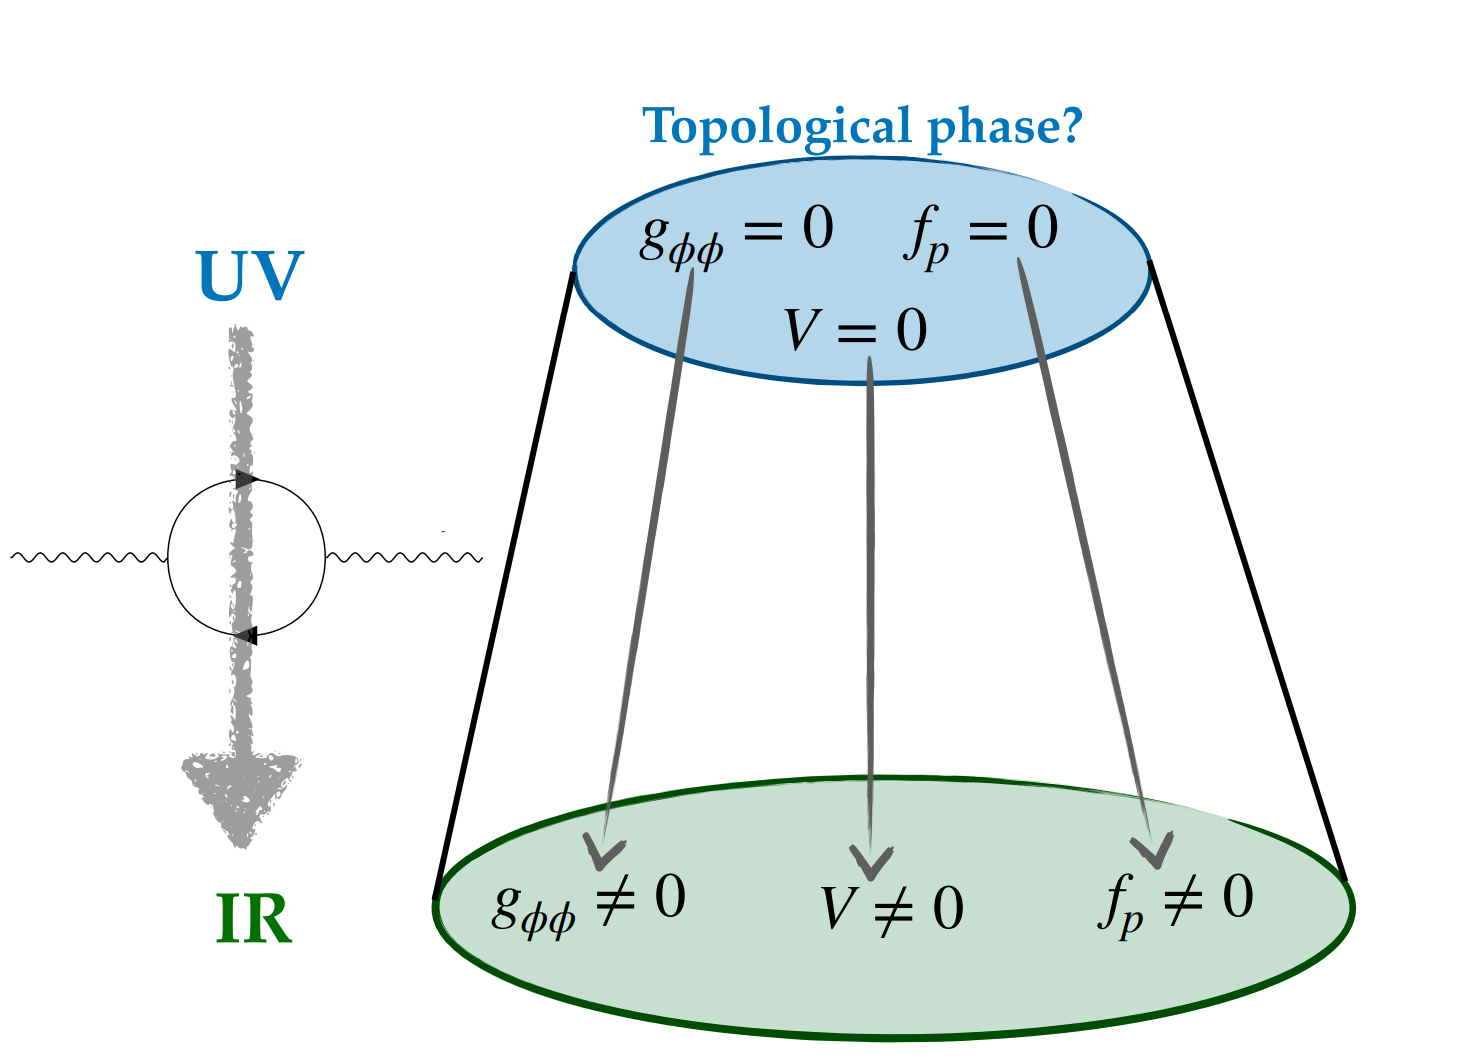
\includegraphics[scale=0.5]{Emergence.png}
			\caption{\AC{Rehacer figura} Scheme of the strong version of the Emergence Proposal. The basic claim is that massless fields would not have any kinetic term in an underlying UV strongly coupled theory and should be regarded as `composite' degrees of freedom (i.e. not elementary). The metrics would be generated by quantum loops involving the contributions due to (infinite) towers of states.}
			\label{fig:strongemergence}
		\end{center}
\end{figure}
%
\end{comment}

\subsection{Emergence of the graviton and the species cut-off}
\label{ss:Emergencegraviton}

One interesting observation that can be drawn at this point concerns the relation between the \emph{perturbative} arguments in favour of the species scale as the quantum gravity cut-off (see Section \ref{ss:perturbative} for details) and the emergence --- in the weaker sense --- of the graviton kinetic term. Indeed, as we elaborated on in Chapter \ref{ch:SpeciesIntro}, any state carrying energy and momentum couples to the gravitational field and in particular it can renormalize the Einstein-Hilbert action, as shown in Figure \ref{fig:oneloopgraviton}. In the following, we would like to make this statement more precise by considering how (towers of) states with different spin --- such as scalars, fermions, vectors, etc. --- contribute to the graviton kinematics at one-loop. For concreteness, let us assume that there is an infinite tower of species with masses $m_1 \leq m_2 \leq \ldots \leq m_N \leq \LSP$ weakly coupled to gravity. For energies well below $m_1$, we can integrate out the tower up to the quantum gravity cut-off, thus obtaining certain threshold corrections to the `bare' Einstein-Hilbert term, which reads as
%
\begin{equation}\label{eq:EH}
	S_{\text{EH},\, \LSP} = \frac{\LSP^{d-2}}{2} \int \dd^{d}x\, \sqrt{-g}\,  \mathcal{R}\, .
\end{equation}
%
Note that in the previous expression we have assumed the reduced Planck mass measured at energies around the cut-off $\LSP$ to be given precisely the species scale itself. Therefore, upon using the worldline formalism\cite{Schubert:2001he, Vassilevich:2003xt, Bastianelli:2008cu,Bastianelli:2005rc} --- which is manifestly gauge invariant --- one finds (see Appendix \ref{ap:heatkernel} for details)
%
\begin{equation}\label{eq:quantumEH}
	S_{\text{EH},\, \text{eff}} = \frac{\LSP^{d-2}}{2} \int \dd^{d}x\, \sqrt{-g}\,  \mathcal{R} \left( 1+\sum_{n=1}^N \gamma_n \right)\, ,
\end{equation}
%
where $\{\gamma_n\}$ comprise some positive $\mathcal{O}(1)$ factors depending both on the statistics and spin of the corresponding field (c.f. eqs. \eqref{eq:dewittcoeffscalar} and \eqref{eq:dewittcoefffermion}). Moreover, if we assume the total number $N$ of such particles to be very large, we can then take the summation to be roughly proportional to the number of species, such that
%
\begin{equation}\label{eq:finalquantumEH}
	S_{\text{EH},\, \text{eff}}\, =\, \int \dd^{d}x\, \sqrt{-g}\,  \left(\frac{N\, \LSP^{d-2}}{2}\, \mathcal{R}\ +\ \mathcal{O}\left(\frac{1}{N} \right)\right)\, ,
\end{equation}
%
which thus defines \emph{a posteriori} the Planck mass measured in the infra-red to be given by $\Mpd^{d-2} := \LSP^{d-2}\, N$. Notice that in order to arrive at \eqref{eq:finalquantumEH} it is indeed crucial that all fields entering into the one-loop computation contribute \emph{positively} to the latter, irrespective of their spin or statistics. This amounts to asking for no `anti-screening' phenomenon to happen in gravitational theories, and is to be expected based on general physical grounds \cite{Anber:2011ut,Donoghue:1994dn, Han:2004wt}.\footnote{Heuristically, the reason for this stems from the fact that the graviton couples to energy, which is positive definite. Furthermore, the modern perspective based on unitary methods (see e.g., \cite{Elvang:2013cua,Kruczenski:2022lot} and references therein) allows one to reconstruct generic loop corrections from tree-level diagrams, which would carry the positivity of the \emph{on-shell} coupling between gravity and energy-momentum \cite{Donoghueprivate}.} Furthermore, let us mention that even in the extreme case where $m_n \approx \LSP$ for all $n \leq N$, one obtains a correction of the form (c.f. eq. \eqref{eq:integratedoneloop})
%
\begin{equation}\label{eq:extremequantumEH}
	\mathcal{L}_{\text{EH},\, \text{eff}}\, \sim\, \sqrt{-g} \left( N\, \LSP^{d-2} E_{\frac{d}{2}} (1)\, \mathcal{R} \right)\, \sim\, \sqrt{-g} \left(\Mpd^{d-2}\, \mathcal{R} \right)\, ,
\end{equation}
%
where $E_{k}(z)$ is the exponential integral function. This means that even if all $N$ species have a mass of order of the quantum gravity cut-off, we still get the desired result \eqref{eq:finalquantumEH}.

%%%%%%%%%%%%%%%%%%%%%%
\begin{figure}[tb]
		\begin{center}
			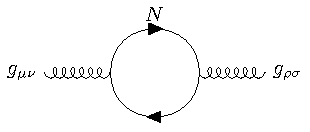
\includegraphics[scale=1.3]{Graviton_Loop.pdf}
			\caption{Contribution of the one-loop determinant of $N$ light species to the graviton self-energy. This can be related to the emergence of the gravitational field, as explained in the text.}
			\label{fig:oneloopgraviton}
		\end{center}
\end{figure}
%%%%%%%%%%%%%%%%%%%%%%

Let us stress at this point that, strictly speaking, one does not need to assume the boundary condition \eqref{eq:EH} at the cut-off scale in order to obtain the correct asymptotic dependence for the Einstein-Hilbert action in the infra-red. Consequently, this would allow for the possibility of fully generating the graviton kinematics via quantum corrections induced by the infinite towers of states, as in the stronger versions of the Emergence Proposal. %\AC{Q: What about higher spin ($s\geq1$) fields? Do they still contribute positively to \eqref{eq:finalquantumEH}? For Emergence to be on the right track they should all contribute positively, in agreement with the perturbative species scale computation. See perhaps \cite{Bastianelli:2008cu,Bastianelli:2005vk,Bastianelli:2005uy} and references therein.}

\subsection{Relation to the Swampland conjectures}
\label{ss:Emergence&Swampland}
	
One attractive feature of the Emergence Proposal is that it provides us with a very simple microscopic rationale for the understanding the existence of both the Weak Gravity and the Distance conjectures \cite{Arkani-Hamed:2006emk,Heidenreich:2015nta,Heidenreich:2016aqi,Montero:2016tif,Andriolo:2018lvp,Ooguri:2006in, Etheredge:2022opl}.\footnote{See also \cite{Stout:2021ubb,Stout:2022phm} for alternative approaches to explain the Distance Conjecture based on information theory.} In order to give a flavour of why this is so, let us consider here a simple toy model in $d > 4$ spacetime dimensions with a BPS-like spectrum of charged particles labeled both by their $\mathsf{U(1)}$ gauge charge $n \in \mathbb{Z}$ and mass $m_n=|n|\, \Mt$, with $|n| \leq N$, where $N$ is effectively very large. We also assume that these massive states couple to a single real modulus $\phi$ through its field-dependent mass, namely $m_n = m_n (\phi)$.

On the one hand, if gravity was no present we could still compute the one-loop contribution to the modulus kinetic term, which we denote by $g_{\phi\phi}$ (see Figure \ref{torresa}). For concreteness, we take the infinite tower to be comprised by e.g., massive fermionic fields $\Psi_n$, whose moduli-dependent mass is controlled by some Yukawa interaction of the type $(\partial_\phi \Mt)\, \phi \ \overline{\Psi^{(n)}} \Psi^{(n)}$. Therefore, upon summing over the whole spectrum we find\footnote{We ignore for the moment some subtleties associated to the precise loop computations which will be explained in upcoming sections. Let us stress though, that the results presented here are essentially unchanged.}
%
\beq \label{eq:metricemergence}
	\delta g_{\phi\phi}\, \sim\, \sum_{n=1}^N n^2 \Lambda_{\text{UV}}^{d-4}  (\partial_\phi \Mt)^2\, \sim\, N \Lambda_{\text{UV}}^{d-2} \left(\frac {\partial_\phi \Mt}{\Mt}\right)^2\, ,
\eeq
%
where we have not kept track of the $\mathcal{O}(1)$ factors that arise either from the loop diagram nor upon performing the finite sum, which has been cut off at an energy scale $\Lambda_{\text{UV}} = N\, \Mt$ beyond which our effective description breaks down. Indeed, we see that a kinetic term is obtained at the quantum level, but it is in principle divergent if one naively insists on taking the continuum limit, i.e. $\Lambda_{\text{UV}} \to \infty$. However, the renormalization prescription will force us to have some (divergent) kinetic term already at the UV scale so as to be able to make finite  physical predictions at low energies. Thus, one cannot simply claim that kinematics is completely induced in the infra-red. 

Similarly, one can easily compute the quantum contributions to the wave-function of the $\mathsf{U(1)}$ gauge boson induced by the tower of charged fermions. As is well-known, this captures the renormalization of the (inverse) gauge coupling, which reads
%
\beq
	\delta \left(\frac {1}{g^2}\right)\, \sim\,  \sum_{n=1}^N n^2 \Lambda_{\text{UV}}^{d-4}\, \sim\, N \Lambda_{\text{UV}}^{d-2} \frac {1}{\Mt^2}\, ,
	\label{eq:gaugecouplingemergence}
\eeq
%
where we are again ignoring any numerical prefactor in \eqref{eq:gaugecouplingemergence}. Notice that, as it was also the case for the scalar field, strictly speaking there is no emergence phenomenon whatsoever, since large kinetic terms must be already present in the UV regime.  

%
\begin{figure}[t]
		\begin{center}
			\subfigure[]{
				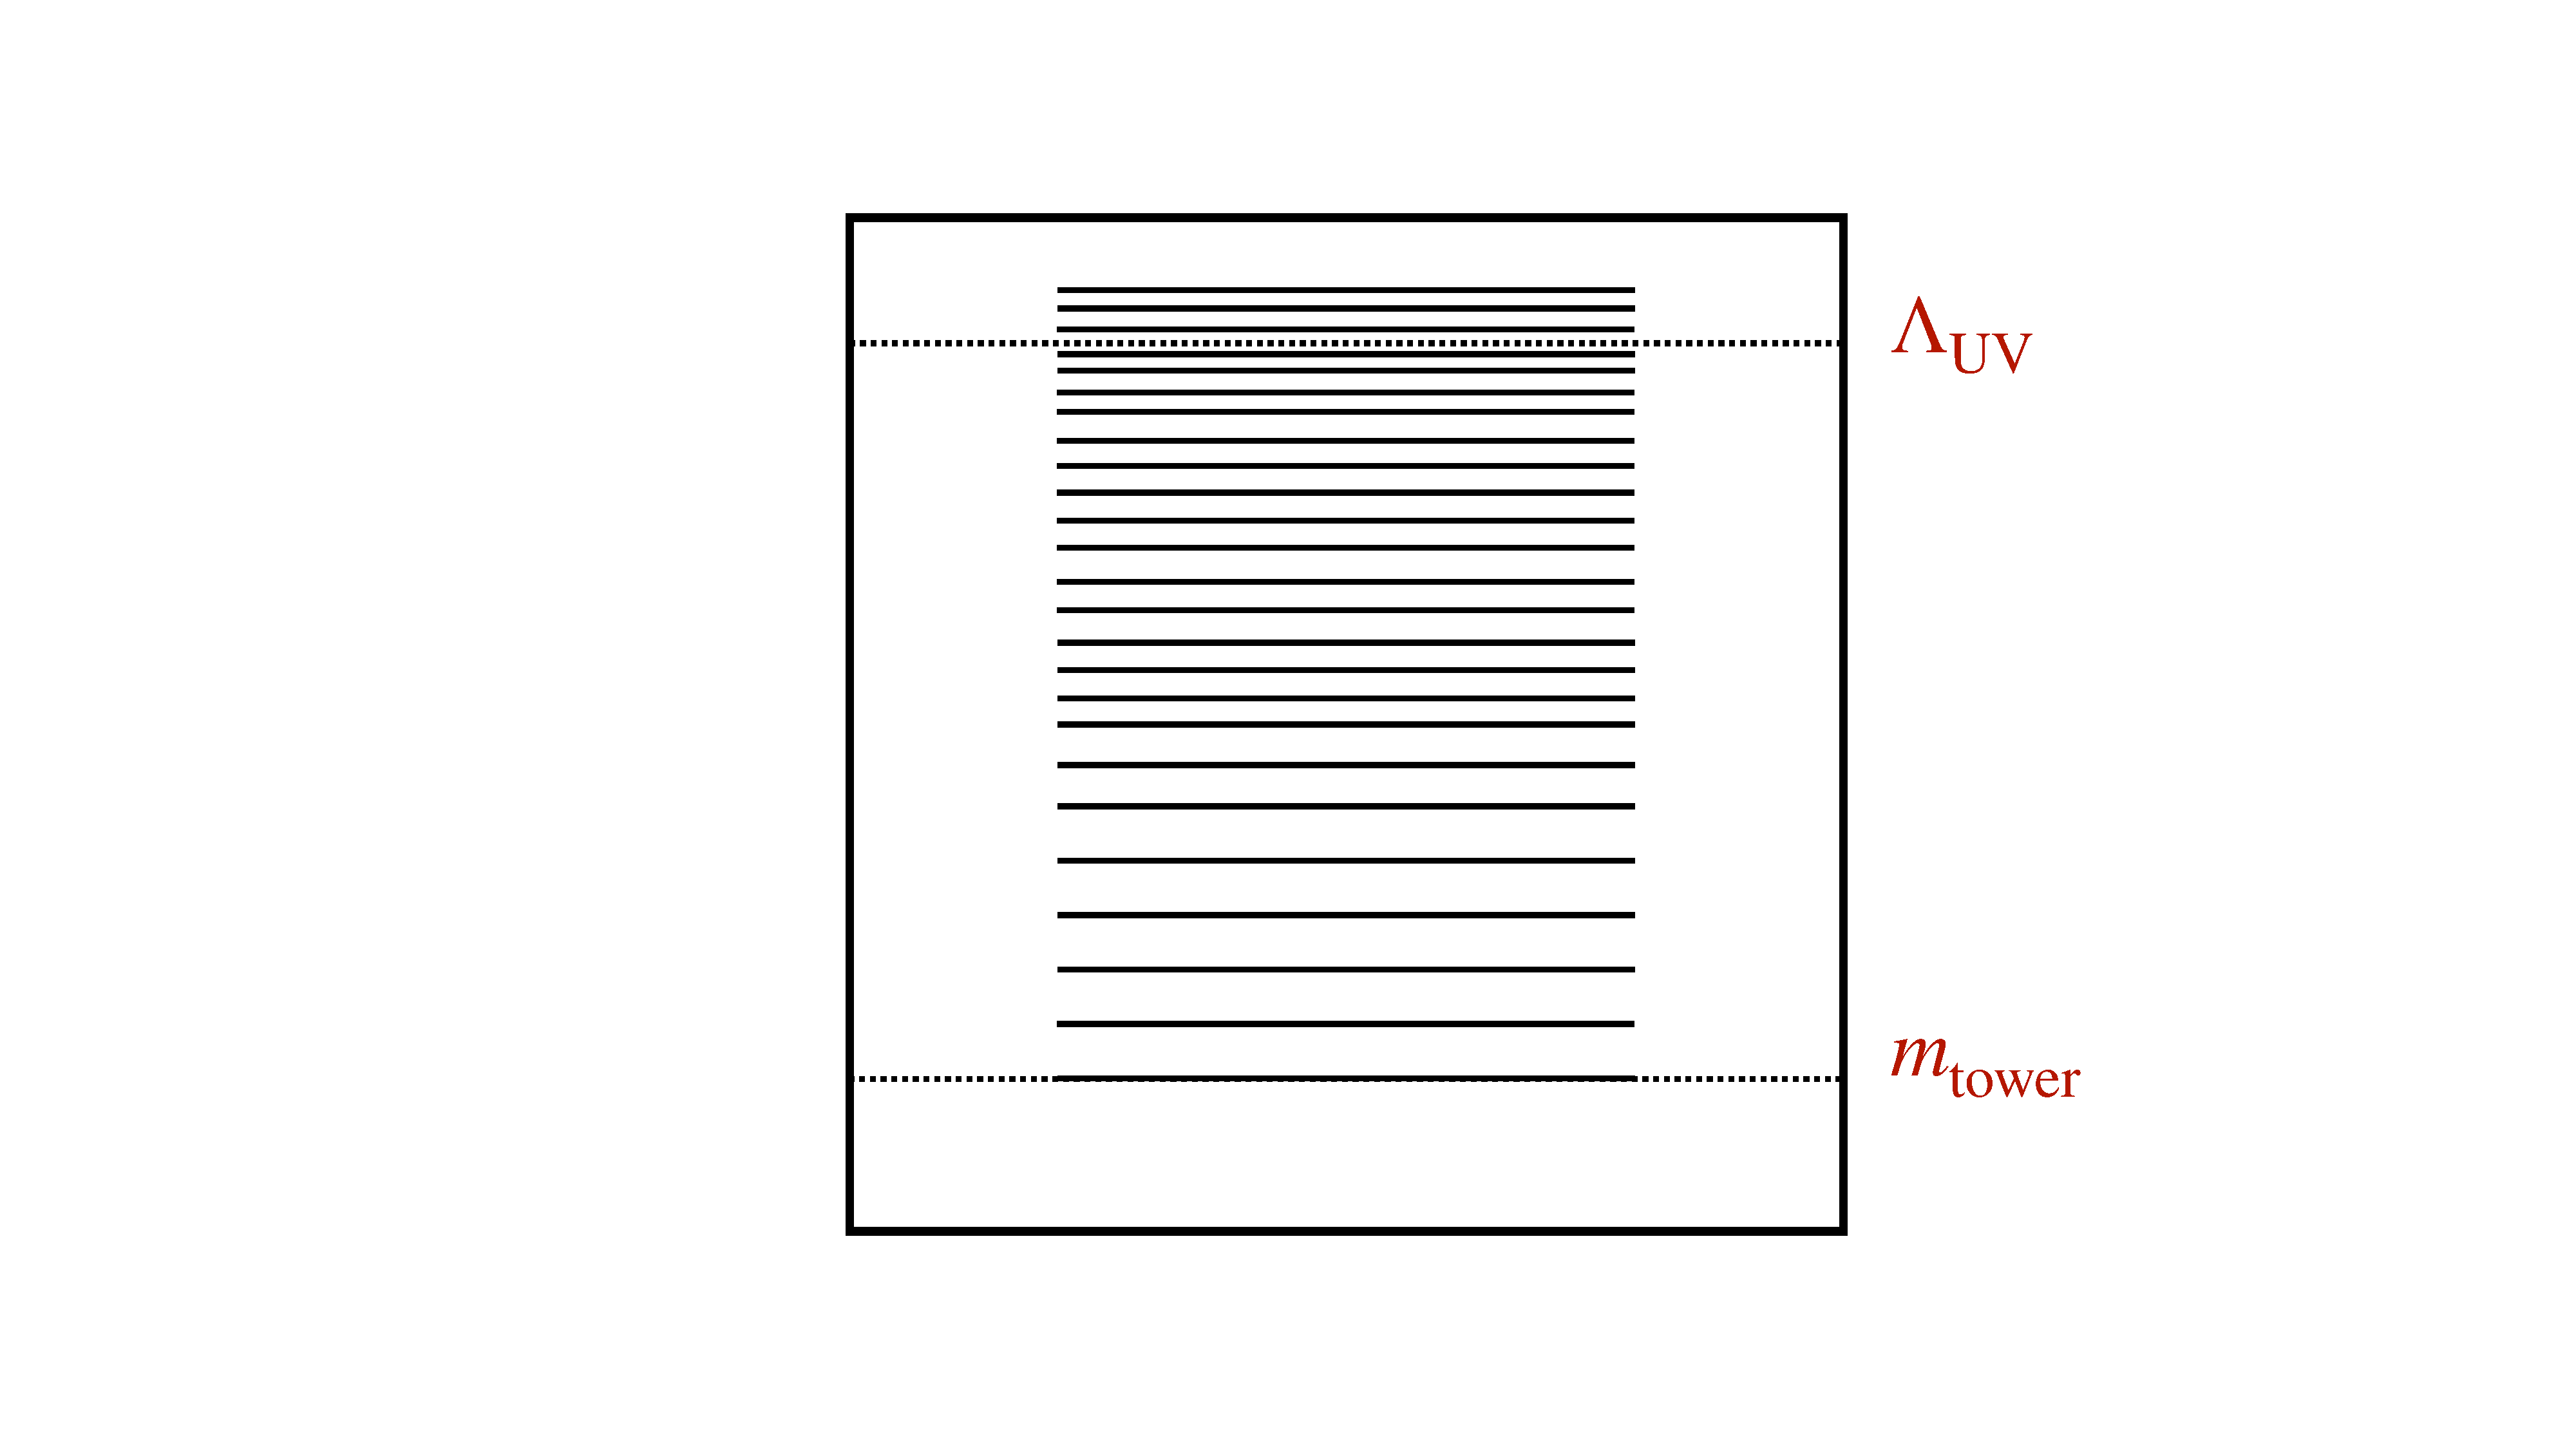
\includegraphics[height=4.0cm]{Emergence_tower_NO_Gravity.pdf} 
				\label{torresa}
			}
			\subfigure[]{
				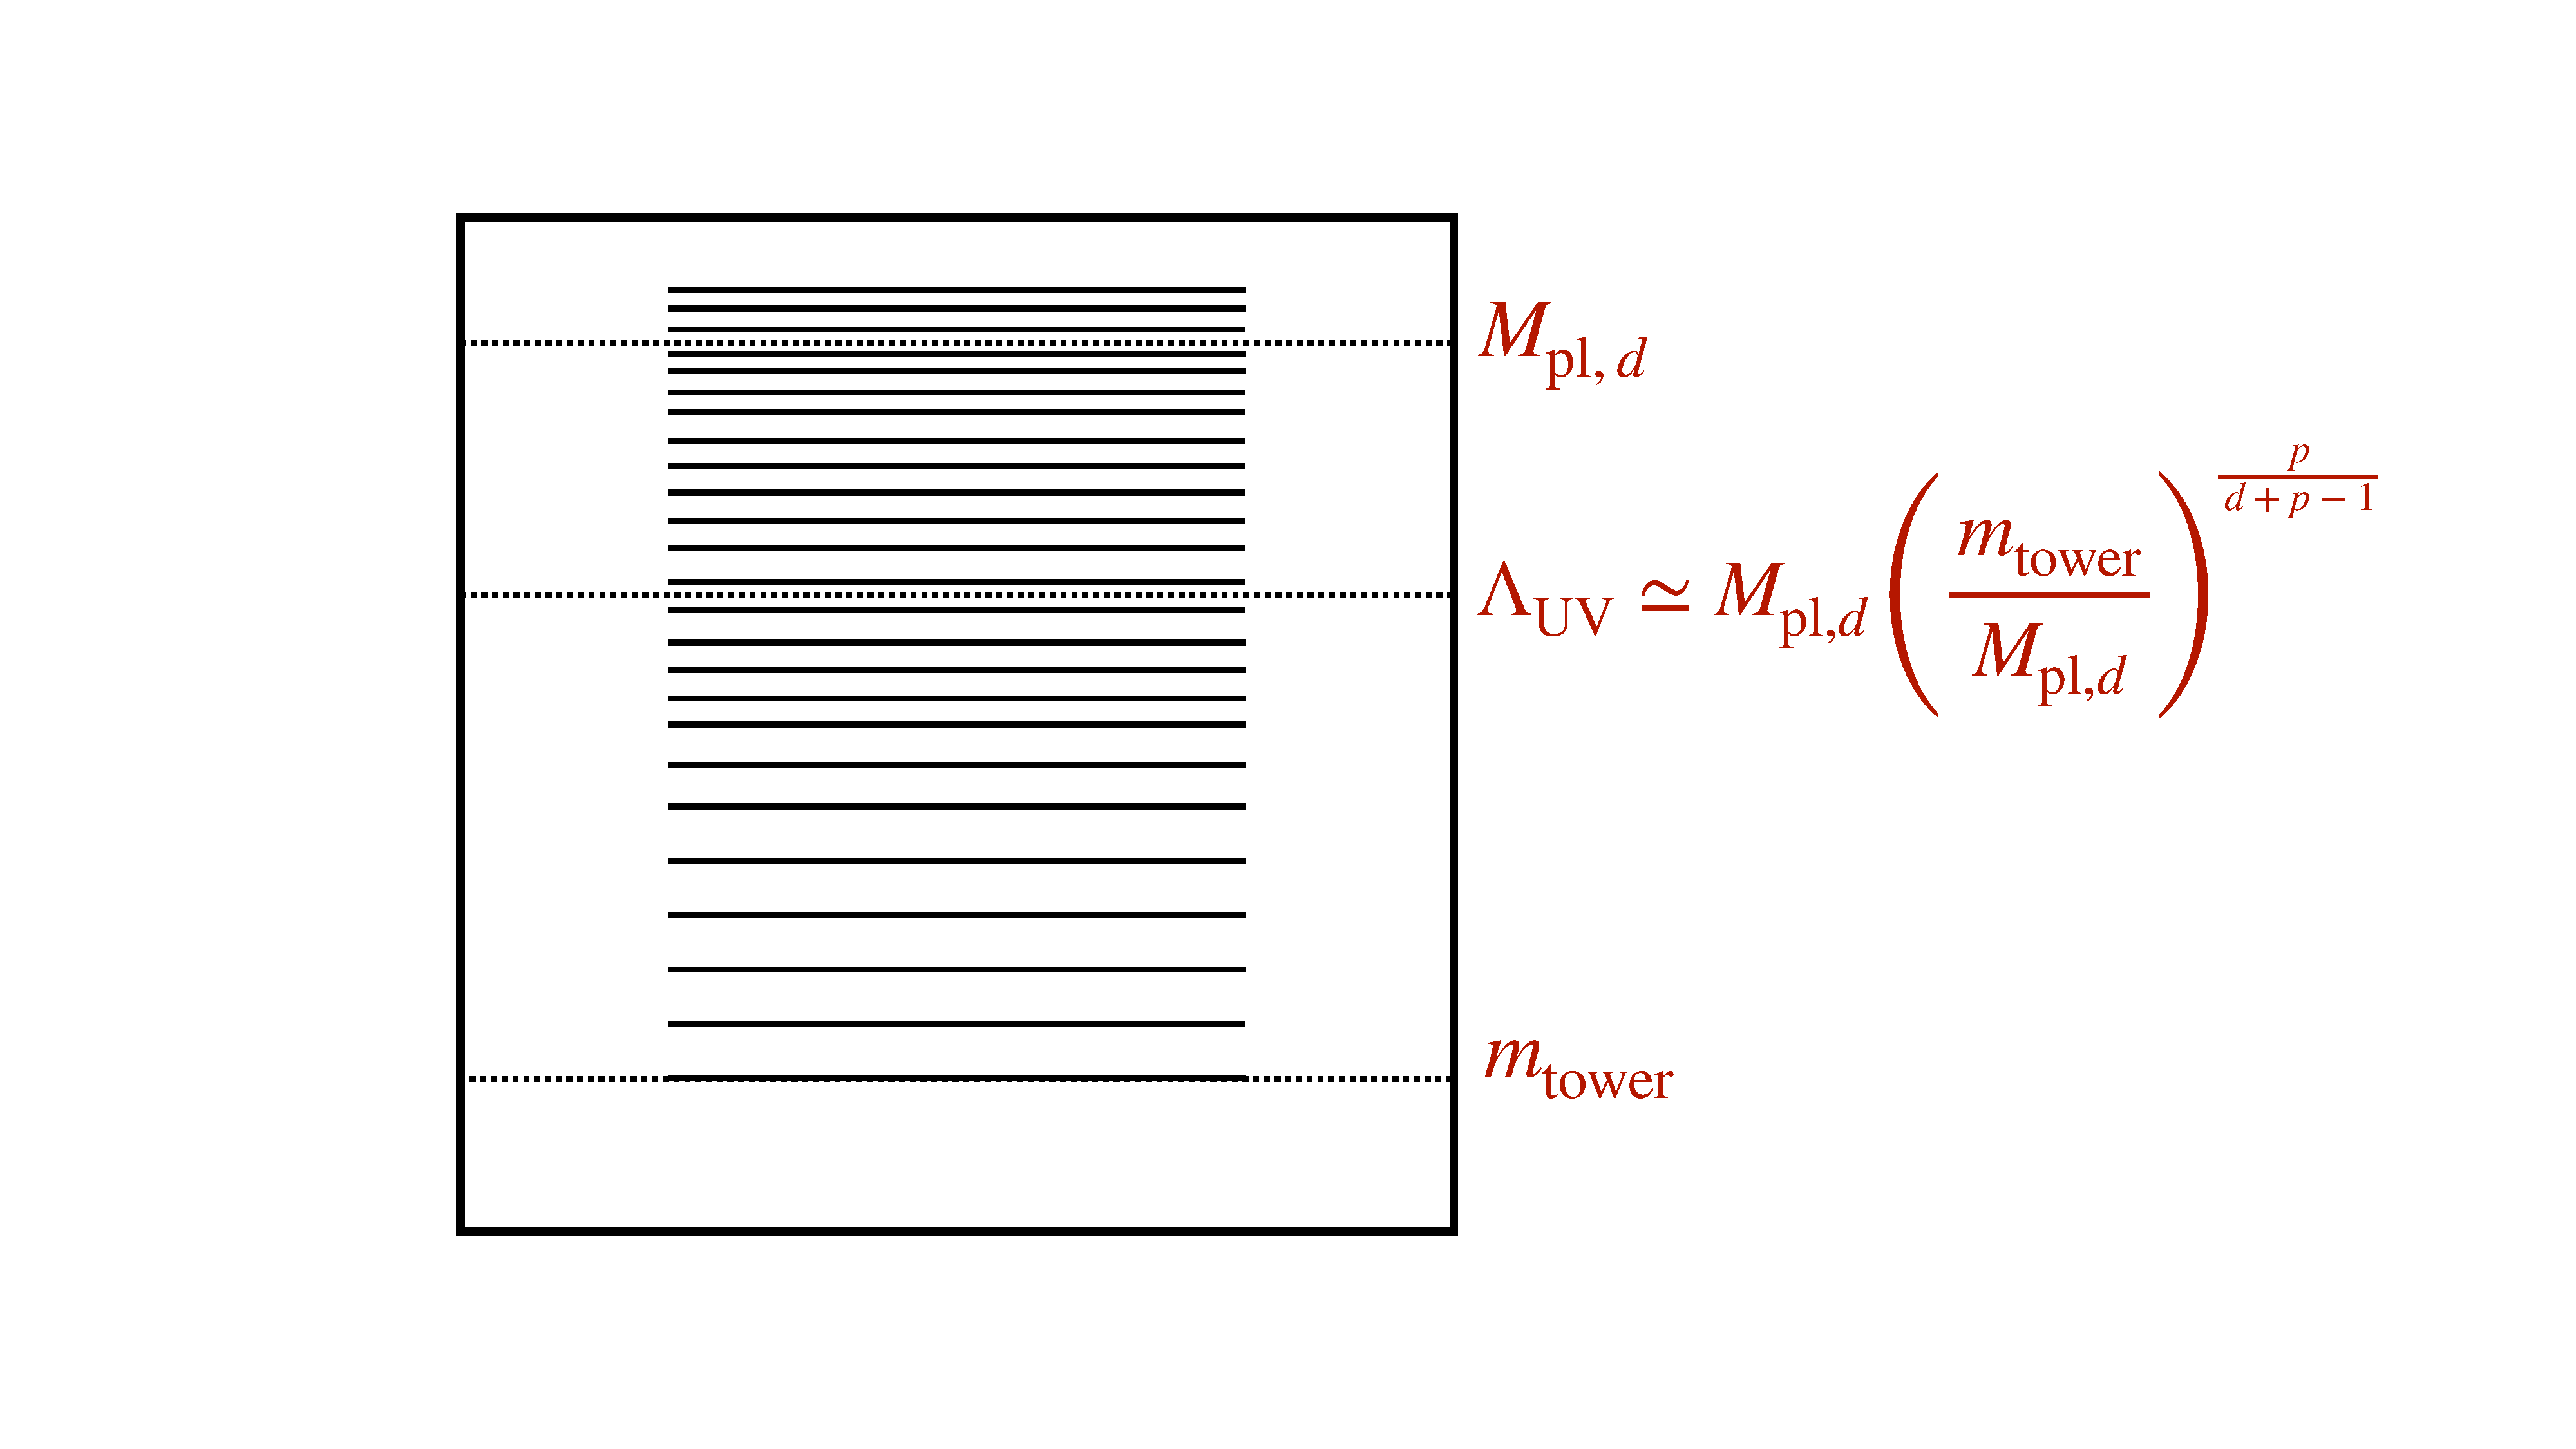
\includegraphics[height=4.0cm]{Emergence_tower_WITH_Gravity.pdf}
				\label{torresb}
			}
			\caption{Emergence of metrics from a tower of states. \textbf{(a)} In the absence of gravity they are sensitive to the cut-off $\Lambda_{\text{UV}}$. \textbf{(b)} In the presence of gravity the UV cut-off must be identified with the species scale. The latter is related to the mass scale of the tower $\Mt$ such that in the end, only $\Mt$ and the Planck mass, $\Mpd$, appear in the EFT.}			
		\label{torres}
		\end{center}
\end{figure} 
%	
Let us now reconsider the previous analysis but now in the context of quantum gravity (see Figure \ref{torresb}). In this case, as already argued in Part \ref{part:QGscale} of the thesis, it makes sense to identify the ultra-violet cut-off $\Lambda_{\text{UV}}$ with the species scale, c.f. eq. \eqref{species}. By doing so, the explicit dependence on the momentum cut-off disappears and one is left with %\footnote{In 4d the leading dependence on the cut-off appears through a logarithmic factor of the form $ \log \left(\LSP^2/\Mt^2 \right)$. However, after further integration over the full tower the final result agrees with the naive expression \eqref{eq:emergencegeneralQG}, which presents no explicit logarithmic dependence on $\LSP$.}
%
\beq\label{eq:emergencegeneralQG}
	g_{\phi\phi}\, \lesssim\,  \Mpd^{d-2}\, \left(\frac {\partial_\phi \Mt}{\Mt}\right)^2\, , \qquad \frac {1}{g^2}\, \lesssim\, \Mpd^{d-2}\, \frac {1}{\Mt^2}\, .
\eeq
%
Consider for the moment the one-loop contribution to the gauge kinetic term given by the second expression above. One thus finds
%
\beq
	\Mt^2\, \sim\, g^2\, \left(N\LSP^{d-2}\right)\, \lesssim\, g^2 \Mpd^{d-2}\, ,
\eeq
%
which exhibits the same qualitative structure as the Weak Gravity Conjecture for a $\mathsf{U(1)}$ gauge field \cite{Arkani-Hamed:2006emk}. In this sense, the emergence of the gauge kinetic term together with the species scale imply the WGC.

Concerning the modulus scalar, once we found the field space metric we can easily compute the distance in moduli space between any two given points, $\phi_a$ and $\phi_b$ (provided of course they lie ultimately at infinite distance from one another, which is where our computations have been done reliably). By doing so, we arrive at 
%		
\beq
\label{eq:distancegeneral}
	\kappa_d\, \Delta\phi_{ab}\, =\,  \kappa_d\, \int_{\tau_a}^{\tau_b} \text{d}\tau \sqrt{g_{\phi \phi}\, \dot{\phi}^2}\, \sim \, \int_{\phi_a}^{\phi_b} \frac {\partial_\phi \Mt}{\Mt}\, d\phi\, \sim \, \log \left(\frac {\Mt (\phi_b)}{\Mt (\phi_a)}\right)\, ,
\eeq
%
where we denote $\dot{\phi}=d \phi/d\tau$, with $\tau$ being some affine parameter, and we have substituted $\kappa_d^2\, g_{\phi \phi} \sim (\partial_\phi \Mt/\Mt)^2$ in eq. \eqref{eq:distancegeneral} above. From here one obtains the sought-after exponential behaviour for the mass scale of the tower, namely
%
\beq
	\Mt (\phi_b)\, \sim\, \Mt(\phi_a)\, e^{-\lambda \kappa_d \Delta\phi_{ab}}\, , \qquad \text{with}\ \lambda=\mathcal{O}(1)\, .
\eeq
%
This is precisely the content of the Distance Conjecture \cite{Ooguri:2006in}.
	
Let us mention that even though the above analysis is framed within a very simple $d$-dimensional example --- with $d>4$, we will see that similar results are attained for more complicated tower structures and different spacetime dimensions, including also the case of string oscillator modes. The take-home message is that the concept of Emergence is intimately related to the Weak Gravity and the Distance conjectures and that in this connection it is crucial that the cut-off in the effective field theory is taken to be the species scale. However, the final expression for the metrics may be written in a way which is independent of the quantum gravity scale (equivalently $N$) and depends explicitly only on `infra-red' data, such as the value of $\Mt$ as well as the Planck mass.
	
	
\subsection{Classical metrics from quantum effects}\label{ss:classicalfromquantum}

As an aside, let us take the opportunity to discuss a subtle point that is raised by our analysis here. This has to do with the fact that the emergence prescription in principle tells us that seemingly \emph{classical} results, such as the tree-level graviton term (c.f. eq. \eqref{eq:EinsteinHilbertaction}), can be generated by summing instead over an infinite number of \emph{quantum} contributions. This naively contradicts our quantum field theory intuition, where the Wilsonian effective action --- or rather any physical quantity derived from it --- can be organized as a perturbative series in $\hbar$, thereby separating classical effects from purely quantum corrections. 

The resolution to this puzzle lies on the very definition of the species cut-off, which is a quantity that is quantum in nature. This can be seen both from the perturbative and non-perturbative analyses presented in Section \ref{s:speciesmotivation}. In any event, after carefully keeping track of the relevant powers of $\hbar$ we arrive at the relation
%
\beq
\begin{aligned}
    \ell_{\rm sp}^{d-2} = \ell_d^{d-2}\, \left(\frac{N}{4\pi} \right) = 8\pi G_N \hbar^{d-3} N\, ,
\end{aligned}
\eeq
%
where crucially $\ell_{\rm sp}$ ends up depending explicitly on Planck's fundamental constant. Therefore, by performing the loop integrals as outlined in Sections \ref{ss:Emergencegraviton} and \ref{ss:Emergence&Swampland} and upon imposing $\LSP$ to be the physical cut-off, we actually obtain fully consistent results (at least from this perspective) where the overall normalization of the kinetic terms is controlled by a factor of $\kappa_d^{-2}$, which is independent of $\hbar$. Hence, even though the Emergence Proposal is quantum in  nature, the species scale comes itself from a purely quantum computation such that both effects ultimately cancel each other, yielding a seemingly classical result.\footnote{The idea that loop corrections in gravity can lead to classical effects in the infra-red is a well-known fact in the literature, see e.g., the recent review \cite{Donoghue:2022eay} and references therein.}

\begin{comment}
	
Above we have argued that combining Emergence and the Species Bound one can obtain the SDC and the magnetic WGC. However, the implications go in all three directions as schematically summarized in Figure \ref{fig:triangulo}. Any two vertices in the triangle imply the third one. Thus, we have already shown how Emergence plus the Species Scale imply the SDC and the magnetic WGC. On the other hand, from eqs. \eqref{eq:metricemergence} and \eqref{eq:gaugecouplingemergence} one concludes that Emergence together with the SDC and magnetic WGC imply the existence of the Species Bound (independently from its possible derivation in terms of graviton loops or rather non-perturbative BH physics, see Section \ref{s:speciesscale}). Finally, one can also argue that it is possible to motivate Emergence in the above simplified setting starting from the SDC, the magnetic WGC and the Species Scale as follows. Thus, assuming the SDC in eq. \eqref{eq:metricemergence} one gets
%
\beq\label{eq:SDCWGC->Emergence}
	\delta g_{\phi\phi}\, \sim\, 
	N \LQG^{d-2} \left(\frac {\partial_\phi m_{\text{tower}}}{m_{\text{tower}}}\right)^2\, \sim\, N^3\LQG^{d-4}(\partial_\phi m_{\text{tower}})^2\, ,
\eeq
%
where we have substituted eq. \eqref{species} and we have used $\LQG \simeq N\, m_{\text{tower}}$. This may be rewritten as the sum over $N$ contributions
%
\beq
	\delta g_{\phi\phi}\, \sim\, \sum_{n=1}^N n^2 \LQG^{d-4}(\partial_\phi m_{\text{tower}})^2\, \sim\, \sum_{n=1}^N (\partial_\phi m_n)^2\LQG^{d-4}\, ,
\eeq
%
where $m_n=n\, m_{\text{tower}}$. But each contribution precisely matches the behaviour of a would-be one-loop graph involving fermions of mass $m_n$ and a Yukawa-like interaction between the tower and the scalar $\phi$ proportional to $\partial_\phi m_n$. Of course this is just a mathematical decomposition of eq. \eqref{eq:SDCWGC->Emergence}, which despite not being unique, is indeed consistent with the Emergence Proposal.
	
	
%
\begin{figure}[tb]
		\begin{center}
			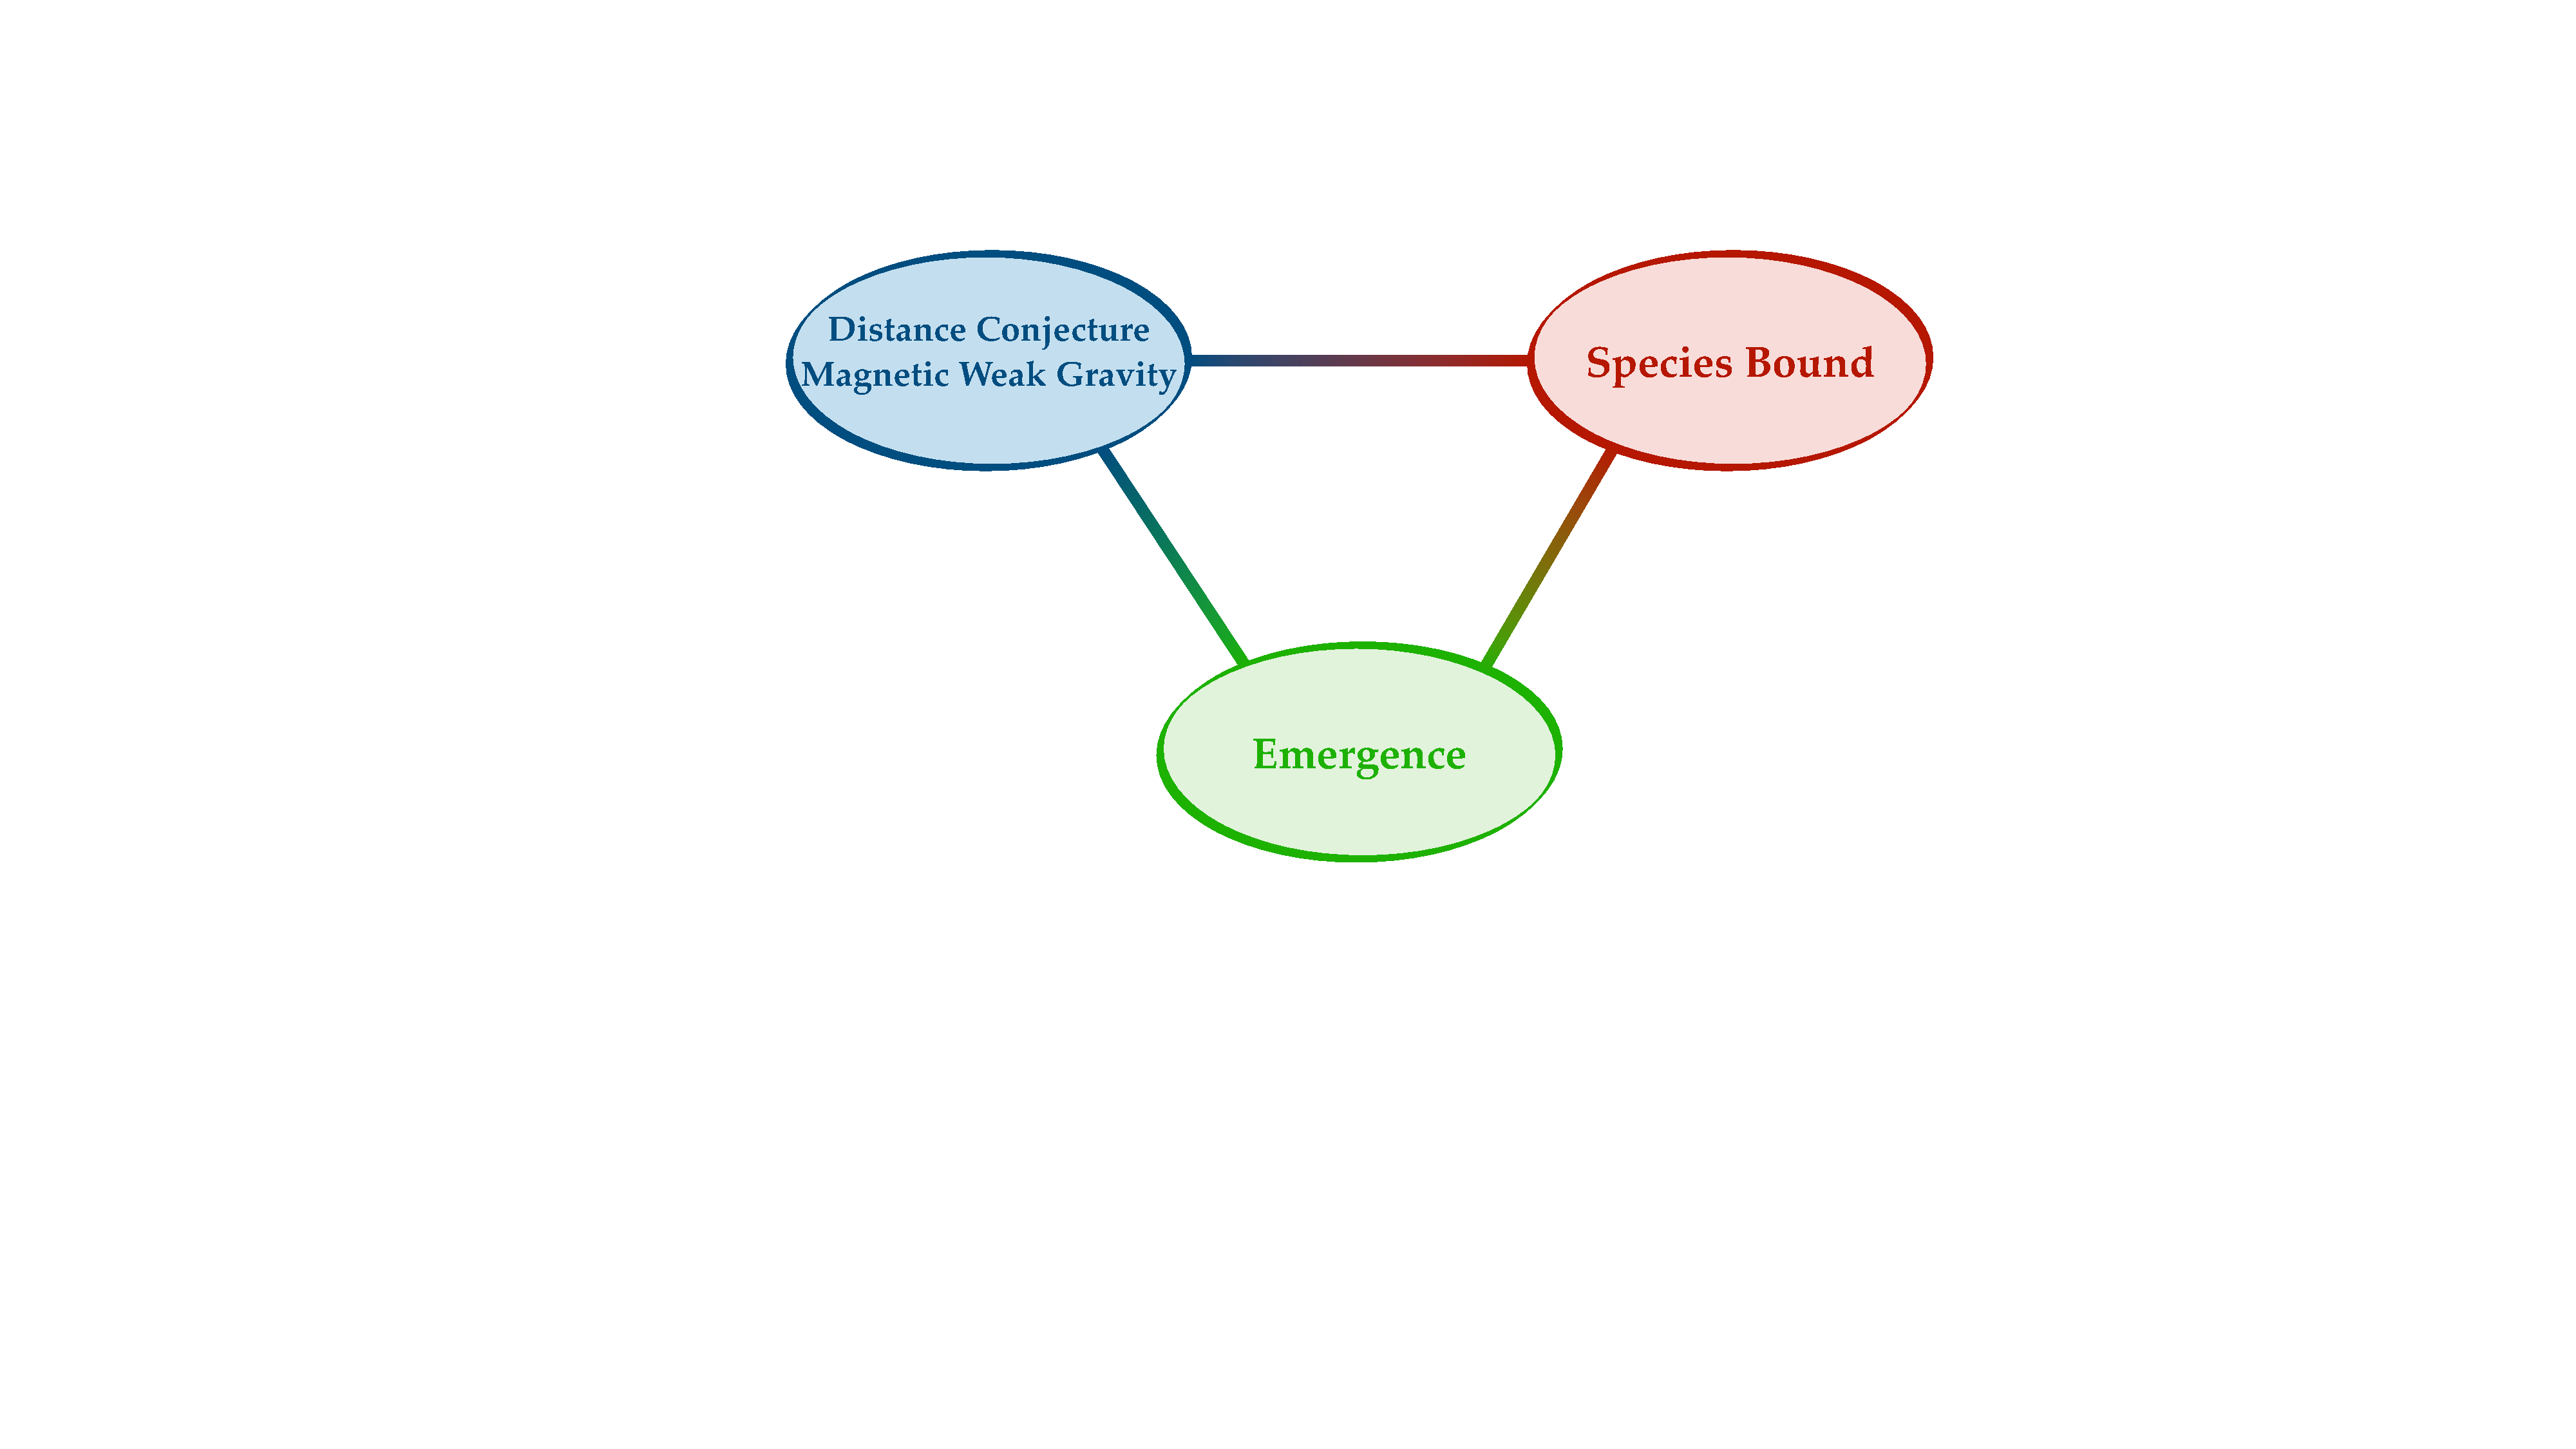
\includegraphics[scale=0.33]{Triangulo.pdf}
			\caption{Connections between the Distance Conjecture, (magnetic) Weak Gravity Conjecture, the Species Bound and Emergence. Any two vertices in the diagram seem to imply the third one.}
			\label{fig:triangulo}
		\end{center}
\end{figure}
%

\subsection{Emergence and String/M-theory}
	
In this paper we will use string/M-theory as a testing ground for the Emergence Proposal, so it is interesting to consider how Emergence fits in here in general terms. In Section \ref{s:EmergenceStringTheory} we analyze several string theory examples of the emergence mechanism in four, six, seven and ten non-compact dimensions. Still, there are some general considerations that one can make before going into the details in each of them. To start with, the case of eleven-dimensional M-theory is rather special because it has no moduli space whatsoever, such that the approach for computing emergent kinetic terms close to infinite distance points that is typically taken cannot be directly applied here. Instead, and especially if the strong version of the Emergence Proposal turns out to be correct and applicable everywhere in Quantum Gravity, we would expect the kinetic terms of M-theory to be understood as well via Emergence but only with the full non-perturbative, UV-complete theory. Alternatively, one could think of 11d M-theory as arising from an asymptotic decompactification limit of 10d Type IIA string theory, in which all kinetic terms may be emergent, as we will discuss below. Therefore, in a sense, M-theory would also fit within the emergence picture. 
	
Emergence is based on the quantum corrections to kinetic terms and one can wonder about what happens in theories with `too many' supercharges (i.e. more than 16), like supersymmetric string theory vacua in $d\geq7$, in which supersymmetry may imply strong cancellations within the loop computations. A first relevant perturbative computation is that of the species scale, which involves corrections to the 2-point function of the graviton due to all kind of light matter fields present in the theory and interacting gravitationally, as described in the previous section. However, due to the fact that in gravity there should be no `anti-screening', namely no negative contributions to the self-energy (at least for point-particles in $d>2$) those graphs could never cancel. This is expected on general physical grounds, but e.g. has been tested in four dimensions in \cite{Anber:2011ut,Donoghue:1994dn, Han:2004wt},\footnote{We acknowledge correspondence on this topic with J. Donoghue.} which suggests it may still be true in higher dimensions, given that one can always consider a trivial toroidal compactification down to 4d starting from any higher dimensional theory. This also agrees with the non-perturvative estimation of the species scale in terms of black holes described in Section \ref{s:speciesscale}, which matches the perturbative one only if this cancellations never occur. In addition, upon assuming this behaviour one naturally concludes that all supersymmetric partners of the graviton, like graviphotons or gravitini, should also have their kinetic terms generated along similar lines. This would be the case e.g. for the RR $1$-form of 10d Type IIA as well as for the graviphoton in 4d $\mathcal{N}=2$ CY$_3$ Type II compactifications. These examples of Emergence, along with others, will be discussed in more detail in Section \ref{s:EmergenceStringTheory}.  
	
Note that for the Emergence Proposal to be correct, it must always lead to `well-defined' kinetic terms. In particular, the \emph{overall} quantum corrections should have the appropriate sign. Therefore, if upon computing such kinetic terms and after having integrated out a tower of states one obtains the wrong sign, self-consistency of the emergence mechanism `predicts' that there should be an additional tower(s) of states that was overlooked and must be included in the computation. Thus, the proposal is far-reaching and should be testable in plenty of string theory vacua.
	
Let us finally comment on the close connection between Emergence and string dualities. Indeed, Emergence is associated to singular limits in the moduli space of the theories under study, those singularities being located at infinite distance. However, there is strong evidence (for Minkowski backgrounds at least) that in these limits one obtains either a decompactification or a string becoming asymptotically tensionless \cite{Lee:2019wij}. Hence e.g., the strings arising are in general different from the original fundamental string considered. Therefore, these singularities correspond in principle to different dualities which exist already in string theory, and the emergence process here discussed would provide (in its strongest formulation) for the kinetics terms of the emergent theory, which appear now typically at the {\it tree level} in the dual frame. A clear example of this process arises in weak coupling regimes of 2-form fields in 6d $\mathcal{N}=(1,0)$ theories, where a nearly tensionless string appears along the limit, as we discuss in Section \ref{ss:emergence6d}.

\end{comment}

\section{Kinetic terms from one-loop corrections}
\label{s:selfenergybosons}	

In this section we discuss the  computation of the wave-function renormalization that an infinite tower of bosonic and/or fermionic particles induce on a given modulus, $p$-form gauge field and massless fermion. For concreteness, we perform such computations for towers comprised by spin-0 scalars and spin-$\frac{1}{2}$ Dirac fields, keeping in mind that we use them as a proxy to estimate the contribution of general towers of scalars and/or fermions to the quantum loops. We outline the basic logic and main results here, leaving the detailed calculations for Appendix \ref{ap:Loops}. In particular, we perform all computations in general $d$ spacetime dimensions, and comment on qualitative differences that arise depending on the latter.

\subsection{Emergence of moduli metrics}
\label{ss:Emergencemodulus}
	
\subsubsection{Self-energy of a modulus field}
\label{sss:selfenergymodulus}
%
\begin{figure}[t]
		\begin{center}
			\subfigure[]{
				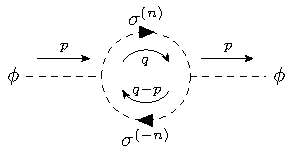
\includegraphics[scale=1.2]{scalarloopscalar.pdf} 
				\label{fig:scalarloopscalar}
			}\qquad \qquad
			\subfigure[]{
				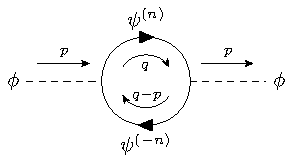
\includegraphics[scale=1.2]{scalarloopfermion.pdf}
				\label{fig:scalarloopfermion}
			}
			\caption{ Contributions to the wave-function renormalization for massless scalars from \textbf{(a)} scalar and \textbf{(b)} fermion loops.}			
		\label{fig:scalarpropagator}
		\end{center}
\end{figure} 
%
	
We begin by considering a real modulus field, $\phi$, coupled to a tower of massive scalars $\{\sigma^{(n)}\}$ or fermions $\{\psi^{(n)}\}$, through their field-dependent masses. The relevant piece of the action can be found in eqs. \eqref{eq:Skinphi}-\eqref{eq:Spsin}. On the other hand, the specific trilinear couplings that enter into the Feynman diagrams contributing to the process are shown in Figure \ref{fig:scalarpropagator}, and can be obtained by expanding the mass term of the states running in the loop up to linear order in the (fluctuation of the) modulus. Their strength is given by
%
\begin{equation}
		\label{eq:scalarcouplings}
		\lambda_n=2m_n(\partial_\phi m_n)\,,  \qquad \mathrm{and} \qquad \mu_n=\partial_\phi m_n \, ,
\end{equation}
%
for massive scalars and fermions, respectively.
	
In the context of Emergence, we are interested in computing the wave-function renormalization of the modulus due to scalar and fermionic loops (see also \cite{Heidenreich:2018kpg, Hamada:2021yxy} for related computations). The idea would be thus to extract the momentum-dependent part of the exact propagator of $\phi$ at one loop, which takes the following form (see Appendix \ref{ap:Loopsscalar} for details)
%
\beq
	\label{eq:scalarpropagator}
	D(p^2)=\frac{1}{p^2-\Pi(p^2)}\, .
\eeq
%
Here, $\Pi(p^2)$ corresponds to the self-energy of the msassless field $\phi$. In the following, we will content ourselves with computing $\Pi(p^2)$ up to $\mathcal{O}(\hbar)$ in the effective action, such that we concentrate on the (amputated) one-loop graph displayed in Figure \ref{fig:scalarpropagator}. (Recall that at tree-level $\Pi_0(p^2)\, = \, 0$.) Thus, the correction to the propagator --- i.e. the modulus metric --- is given by the term in $\Pi(p^2)$ proportional to $p^2$, namely
%
\begin{equation}\label{eq:metriccorrection}
		\delta g_{\phi \phi}= \frac {\partial \Pi(p^2)}{\partial p^2} \bigg\rvert_{p=0}\, .
\end{equation}
%
	
\subsubsection*{Scalar loop}
	
Let us consider first the contributions coming from massive real scalar fields $\{\sigma^{(n)}\}$ corresponding to the Feynman diagram displayed in Figure \ref{fig:scalarloopscalar}, which reads
%
\beq
	\Pi_n(p^2) \ = \frac{\lambda_n^2}{2} \int \frac {\text{d}^dq}{(2\pi)^d} \frac {1}{(q^2+m_n^2)} \frac {1}{((q-p)^2+m_n^2)}\, ,
	\label{eq:selfenergyscalar}
\eeq
%
with the coupling $\lambda_n$ defined in \eqref{eq:scalarcouplings}. In order to compute $\delta g_{\phi \phi}$ we need to extract the term linear in $p^2$ from the expression above, which leads to the following integral in momentum space
%
\beq
	\frac {\partial \Pi_n(p^2)}{\partial p^2} \bigg\rvert_{p=0}  = - \frac{\lambda_n^2}{2} \int \frac {\text{d}^dq}{(2\pi)^d} \frac {1}{(q^2+m_n^2)^3}\, .
	\label{eq:sigmaa}
\eeq
%
From this one can already anticipate the different behaviour in terms of convergence of the momentum integral depending on whether $d$ is equal, lower than, or greater than 6. Even though for $d<6$ the loop integral is convergent for large $q$, we introduce here a momentum cut-off (that will be identified ultimately with the species scale), since this is required for later consistency once we fix the energy scale up to which we include the contribution from the states in the tower that is integrated out. The exact solution of \eqref{eq:sigmaa} is given in terms of hypergeometric functions (c.f. eq. \eqref{eq:scalarloopscalarexact}), but we will focus here on the dependence of the \emph{leading} term on the relevant energy scale (i.e. either the mass of the particle, $m_n$, or the UV cut-off, $\Lambda$), since these are the ones from which we will eventually extract the field dependence of the emergent kinetic terms. In particular, there are two relevant cases in which we are interested: \emph{(i)} The limit $\Lambda \gg m_n$, in which the mass of the particle running in the loop is negligible with respect to the UV cut-off, and \emph{(ii)} $\Lambda\simeq m_n$, where both are roughly of the same order. The former is relevant for most states of KK-like towers in asymptotic regimes, since as we saw in Chapter \ref{ch:SpeciesIntro} the mass scale of the tower is typically parametrically lighter than the species scale. The latter is relevant for the highest modes in KK-like towers and for most states in stringy-like towers, since the masses of the corresponding particles coincide asymptotically with the species scale. Luckily, both limits give rise to the same functional dependence on either $\Lambda$ or $m_n$ (c.f. Appendix \ref{ap:Loopsscalar}), where the expressions only differ in the numerical prefactors.\footnote{To be precise, the numerical coefficients shown in Appendix \ref{ap:Loops} can be thought of as upper and lower bounds on the contributions from each particle in the loop, since they include the two limiting cases for the mass of the relevant particles.} From the results summarized in Tables \ref{tab:scalarloopscalarLambda>>m} and \ref{tab:scalarloopscalarLambda=m} we can thus extract the following asymptotic dependence for the dominant contribution to the 2-point function of the massless scalar $\phi$
%
\begin{equation}\label{eq:scalarloopscalarssummary}
		\frac {\partial \Pi_n(p^2)}{\partial p^2} \bigg\rvert_{p=0}\,   \sim 
		\left\{\begin{array}{lr}
			-  \dfrac{\lambda_n^2}{m_n^{6-d}} & \qquad\text{for } d< 6\, ,\\ \\ 
			-\lambda_n^2 \ \log \left( \dfrac{\Lambda^2}{m_n^2}\right) &\qquad \text{for } d= 6\, ,\\ \\ 
			-\lambda_n^2 \ \Lambda^{d-6}&\qquad \text{for } d>6\, ,
		\end{array}\right.
\end{equation}
%
where the precise meaning of $\sim$ is that we keep track of all the quantities that are field dependent and neglect only the numerical prefactors. %Note that the computation for a scalar loop  was also done in \cite{Hamada:2021yxy} and their results are in agreement with ours.
	
Before proceeding with the fermionic loop, let us make some comments about possible natural generalizations of the scalar case just discussed. First, as typically happens in supersymmetric theories, one could consider a tower of \emph{complex} scalar fields coupled to the modulus $\phi$ through its mass. This scenario reduces essentially to the one described here, since one can always write a complex field in terms of its real and imaginary parts
%
\begin{align}
    \chi^{(n)}=\frac{\sigma^{(n)}_1+\i\sigma^{(n)}_2}{\sqrt{2}}
\end{align}
%
which both share the same moduli-depenedent mass and thus contribute to the self-energy \eqref{eq:metriccorrection} as summarized in eq. \eqref{eq:scalarloopscalarssummary} above (with an extra factor of 2). Second, one could even study the case in which the modulus itself is complexified, namely $\phi \to \Phi = \text{Re}\, \Phi + \i\, \text{Im}\, \Phi$. The scalar charges \eqref{eq:scalarcouplings} would now be complex-valued, and similar considerations would lead to the one-loop generated metric $\delta g_{\Phi \bar \Phi}$.\footnote{Notice that the fact that one obtains a hermitian metric at one loop is due to the pseudo-scalar nature of the imaginary part of the modulus, which prevents a term of the form $(\partial \text{Re}\, \Phi)(\partial \text{Im}\, \Phi)$ from appearing in the effective action.}
	
	
\subsubsection*{Fermionic loop}
	
We consider now the contribution to the propagator from a loop of massive fermions $\{\psi^{(n)}\}$ with trilinear couplings $\mu_n$ as defined in \eqref{eq:scalarcouplings}. The relevant Feynman diagram, shown in Figure \ref{fig:scalarloopfermion}, reads as follows
%
\begin{equation}
		\label{eq:selfenergyfermion}
		\Pi_n(p^2) \, = \, -\mu_n^2  \int \frac {\text{d}^dq}{(2\pi)^d}\ \text{tr} \left (\frac {1}{\i \slashed{q}+m_n}\ \frac {1}{\i (\slashed{q}-\slashed{p})+m_n} \right) \, .
\end{equation}
%
After performing the relevant traces and rearranging terms (c.f. around eq. \eqref{eq:scalarloopfermionstraces} for details), we get the following  expression for the one-loop contribution to the wave-function renormalization 
%
\begin{equation} \label{eq:wfrfermionloop}
		\frac{\partial \Pi_n(p^2)}{\partial p^2} \bigg\rvert_{p=0} \, = \,   -\mu_n^2\, \fdim  \int \frac {\text{d}^dq}{(2\pi)^d} \frac{1}{(q^2+m_n^2)^2} \ + \ 2 m_n^2 \, \mu_n^2\ \fdim \int \frac {\text{d}^dq}{(2\pi)^d} \frac{1}{(q^2+m_n^2)^3} \, .
\end{equation}
%
The first term is negative and looks very analogous to the scalar contribution, with the difference that it naively diverges for $d\geq 4$ instead of $d\geq 6$. Performing a similar analysis as for the scalar loop, we obtain akin results (see Appendix \ref{ap:Loopsscalar}). Namely, for the two limits of interest, $\Lambda \gg m_n$ and $\Lambda \simeq m_n$, we get the same functional dependence on the coupling constants and the pertinent energy scales. The only difference being the numerical prefactors, that play no role in determining the field-dependent part of the emergent metric. The detailed results are summarized in Tables \ref{tab:scalarloopfermionLambda>>m} and \ref{tab:scalarloopfermionLambda=m}, which take the schematic form
%
\begin{equation}\label{eq:scalarloopfermionssummary}
		\frac {\partial \Pi_n(p^2)}{\partial p^2} \bigg\rvert_{p=0}\,   \sim 
		\left\{\begin{array}{lr}
			-  \dfrac{\mu_n^2}{m_n^{4-d}} & \qquad\text{for } d< 4\, ,\\ \\ 
			-\mu_n^2\ \log \left( \dfrac{\Lambda^2}{m_n^2}\right) &\qquad \text{for } d= 4\, ,\\ \\ 
			-\mu_n^2\ \Lambda^{d-4}&\qquad \text{for } d>4\, .
		\end{array}\right.
\end{equation}
%
On the other hand, the second term in \eqref{eq:wfrfermionloop} is of the same form as the scalar contribution \eqref{eq:sigmaa}, with $\lambda_n= 2 m_n (\partial_\phi m_n)=2 m_n \mu_n$, including also a prefactor of $\fdim$ which takes into account the number of fermionic degrees of freedom in $d$ spacetime dimensions. Moreover, it has the opposite sign as the scalar contribution, so for supersymmetric theories both terms cancel and the leading contribution to the emergent metric comes from the first term in \eqref{eq:wfrfermionloop}. For instance, in 4d a single Dirac fermion seems to cancel the renormalization due to two complex --- or four real scalar fields, so that e.g., in 4d $\mathcal{N}=2$ a hypermultiplet only contributes to the modulus metric through the fermion loop.\footnote{A similar cancellation (this time exact) occurs for the would-be mass term generated for the modulus in case supersymmetry is preserved in our theory, which can be checked explicitly upon using our formulae, although one may need to consider some extra loop diagrams not contributing to the wave-function renormalization and therefore not displayed in Figure \ref{fig:scalarpropagator}.} This suggests that following the leading order contribution coming from fermionic towers may be a good proxy for keeping track of the behaviour exhibited by the emergent kinetic terms.
	
	
\subsubsection{Generating moduli metrics}
\label{sss:emergencemodulimetric}
	
Armed with the above results, we study now the emergence of the kinetic term for real scalar moduli in the two relevant scenarios of decompactification and emergent string limits. For the latter, given the lack of a manifestly off-shell formulation of string theory as of today,\footnote{See \cite{Ahmadain:2022tew,Ahmadain:2022eso} though for recent proposals to alleviate this problem.} we will perform the computation using a purely field-theoretic approach, following the perturbative discussion of Section \ref{sss:stringtowersspecies}. Hence, the results there should be taken with a grain of salt. 
	
\subsubsection*{Moduli metrics from  Kaluza-Klein towers}
	
Let us consider a KK-like tower of scalars with mass spectrum and associated species scale given by
%
\beq\label{eq:@@@}
	m_n\, =\, n^{1/p}\, \Mt \, , \qquad   \LSP\,  \simeq\, N^{1/p}\, \Mt \, ,
\eeq
%
so that e.g., a single KK tower would correspond to $p=1$ (see Section \ref{ss:MultipleTowers} for precise definitions). Note that an analogous analysis can be performed with fermionic towers and similar results are obtained. The  contribution of a single scalar to the wave-function renormalization of a modulus field is given in \eqref{eq:scalarloopscalarssummary}, and for $d>6$ it takes the form
%
\beq
	\delta g_{\phi\phi}^{(n)}\, \sim\,  \mathcal{A}_d\, \lambda_n^{2}\, \Lambda^{d-6}\, \sim\, 4\, \mathcal{A}_d\, m_n^2\, (\partial_\phi m_n)^2\, \Lambda^{d-6}\, ,
\eeq
%
with $\mathcal{A}_d$ being a numerical prefactor depending only on $d$ that is not explicitly included in eq. \eqref{eq:scalarloopscalarssummary}. Its precise value for the two relevant limits is displayed in Tables \ref{tab:scalarloopscalarLambda>>m} and \ref{tab:scalarloopscalarLambda=m}. After adding up the contribution from the states of the tower below the cut-off $\Lambda = \LSP $, we get
%
\beq \label{eq:KKloopscalarmetricd>6}
	\delta g_{\phi\phi} \,=\, \sum_{n=1}^{N} \delta g_{\phi \phi}^{(n)}  \, \sim\, \frac {4 p \mathcal{A}_d}{p+4}\,  N^{\frac{4}{p}+1}\,  (\partial_\phi \Mt)^2\, \Mt^2\, \LSP^{d-6}\, \sim\, \frac {4 p \mathcal{A}_d}{p+4}\, \Mpd^{d-2} \left( \frac{\partial_\phi \Mt}{\Mt}\right)^2\, ,
\eeq
%
where we have used $N \simeq\Mpd^{d-2}/ \LSP^{d-2}$ as well as the second relation in \eqref{eq:@@@}. Thus, the non-trivial dependence on the characteristic mass of the tower, namely $\delta g_{\phi\phi} \sim 1/\Mt^2$, is recovered for any dimension, leading to the structure needed for the Distance Conjecture to hold a posteriori. Notice that the dependence on the tower density parameter, i.e. $p \in \mathbb{R}$, only enters through the numerical prefactor in \eqref{eq:KKloopscalarmetricd>6}, so that it is irrelevant for our purposes here.

For $d<6$, on the other hand, the correction associated to one real massive scalar in the loop integral is of the form
%
\beq
	\delta 
	g_{\phi\phi} ^{(n)}\, \sim\, \mathcal{B}_d\, \lambda_n^2\,  m_n^{d-6}\, \sim\, 4\, \mathcal{B}_d\, n^{\frac{d-2}{p}}\, \Mt^{d-4}\, (\partial_\phi \Mt)^2\, .
\eeq
%
Again, $\mathcal{B}_d$ is a $d$-dependent numerical prefactor whose precise value is bounded by the ones shown in Tables \ref{tab:scalarloopscalarLambda>>m} and  \ref{tab:scalarloopscalarLambda=m}. The total contribution from a tower up to the species scale therefore reads
%
\beq 
	\delta g_{\phi\phi}\,=\, \sum_{n=1}^{N} \delta g_{\phi \phi}^{(n)}\, \sim\, \frac {4p\mathcal{B}_d}{d-2+p}\, N^{\frac{d-2+p}{p}}\, \Mt^{d-4}\, (\partial_\phi \Mt)^2\, \sim\, \frac {4p\mathcal{B}_d}{d-2+p}\, \Mpd^{d-2} \left( \frac{\partial_\phi \Mt}{\Mt}\right)^2\, ,
\eeq
%
so that essentially we arrive at the same expression as for $d>6$, with a different numerical coefficient. A similar behaviour is obtained for the marginal case $d=6$ up to a numerical prefactor.
	
\subsubsection*{Moduli metrics from stringy towers}
As a second example, we consider this time the coupling of a real modulus $\phi$ to the oscillator modes of some fundamental string. For concreteness, we choose to do the computation for the fermionic modes only, although the same analysis may be repeated using the bosons yielding similar results as well. Let us study first the case $d>4$. Consider the spectrum of a string with masses and degeneracies for fermionic excitations given by
%
\beq
	m_n^2 = 16 \pi^2 (n-1) \Ms^2\, , \qquad  d(n)\, \sim\,  n^{-b}e^{a\sqrt{n}}\, ,
\eeq
%
where $a$ and $b$ are constants characteristic of each string, see e.g., eq. \eqref{eq:exactleveldensitystrings}. For simplicity, we will approximate in this section $d(n) \sim e^{\sqrt{n}}$, since this is enough for our purposes and the results are already reliable up to log corrections. We moreover assume the string scale $\Ms$ to depend on $\phi$ when measured in Planck units, as indeed happens in string theory (c.f. eq. \eqref{eq:ddimdilaton}). Then the total contribution for the metric arising from fermion loops is 
%
\beq
	\delta g_{\phi \phi}\, \sim\, \sum_{n=1}^{\Ns}\mu_n^2\, d(n)\, \LSP^{d-4} \sim \sum_{n=1}^{\Ns} (\partial_\phi \Ms)^2\, n\, d(n)\, \LSP^{d-4}\, .
\eeq
%
Recalling as well that $\LSP ^2 \simeq \Ns\, \Ms^2$, one finds
%
\beq
	\delta g_{\phi \phi}\, \sim\, \Ms^{d-4}\Ns^{\frac{d-4}{2}} (\partial_\phi \Ms)^2\int^{\Ns}_1 dn\, n\;  e^{\sqrt{n}} \sim  \Ms^{d-4} \Ns^{\frac{d-4}{2}} (\partial_\phi \Ms)^2  \Ns^{3/2}e^{\sqrt{\Ns}}\, .
\eeq
%
Using now the expression \eqref{eq:maxstringlevel}, we finally get
%
\beq\label{eq:modulusWFstringtow}
	\delta g_{\phi \phi}\, \sim\, \frac {(\partial_\phi \Ms)^2}{\Ms^2}\Mpd^{d-2}\, ,
\eeq
%
which is again the expected asymptotic behaviour. Note that the explicit dependence on $\Ns$ drops out, and the result only depends on the mass of the lightest string excitation $\Ms$, as it happened with the Kaluza-Klein towers. It is easy to check that \eqref{eq:modulusWFstringtow} is also reproduced for $d\leq 4$. %An analogous analysis may be performed using the bosonic loop instead of the fermionic one, yielding similar results.

 \subsection{Emergence of $\mathsf{U(1)}$ gauge kinetic terms}\label{ss:EmergenceU(1)gauge}
	
\subsubsection{Self-energy of a gauge 1-form}
\label{sss:selfenergy1form}
%
\begin{figure}[t]
		\begin{center}
			\subfigure[]{
				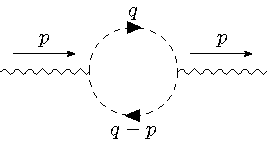
\includegraphics[scale=1.2]{1-formloopscalar.pdf} 
				\label{fig:1-formloopscalar}
			}\qquad \quad 
			\subfigure[]{
				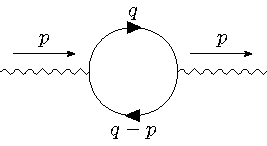
\includegraphics[scale=1.2]{1-formloopfermion.pdf}
				\label{fig:1-formloopfermion}
			}
			\caption{Wave-function renormalization at one-loop for $\mathsf{U(1)}$ gauge bosons due to \textbf{(a)} charged scalars and \textbf{(b)} fermionic fields.}			
			\label{fig:1-formpropagator}
		\end{center}
\end{figure} 	
%
Let us now consider the contribution coming from loops of complex scalar fields $\{\chi^{(n)}\}$ and Dirac fermions $\{\psi^{(n)}\}$ to the propagator of a gauge 1-form, denoted $A_1$. In particular, we take the mass and charge of the $n$-th scalar/fermion to be given by $m_n$ and $q_n$, respectively, whereas the gauge coupling associated to the 1-form is denoted by $g$ (c.f. eqs. \eqref{eq:SkinA1}-\eqref{eq:SpsinA1} for details on the conventions and the precise spacetime action).
	
As in the modulus scenario analyzed in Section \ref{sss:selfenergymodulus}, in order to compute the emergent gauge kinetic terms we must study the relevant Feynman diagrams that contribute to the wave-function renormalization of $A_1$. Subsequently, we need to extract the momentum-dependent part of the exact propagator, after taking into account the one-loop corrections. We choose to use the Lorenz gauge $\partial_\mu A^{\mu}\, =\, 0$ for convenience, since it can be easily generalized to higher $p$-forms as $\partial_\mu A^{[\mu \nu_1 \ldots \nu_{p-1}]}\, = \, 0$. In this gauge, the propagator for the 1-form can be written as
%
\begin{equation}
		\label{eq:A1propagator}
		D^{\mu \nu} (p^2) \, = \, \left( \dfrac{p^2}{g^2} \delta ^{\mu \nu} - \Pi^{\mu \nu}(p^2) \right)^{-1}\, ,
\end{equation}
%
where $\Pi^{\mu \nu}(p^2)$ vanishes at tree-level since it is the amputated Feynman diagram coming from the loops shown in Figure \ref{fig:1-formpropagator}. By imposing again our gauge choice, we can extract the tensorial dependence on
%
\begin{equation}
		\label{eq:A1loopamplitude}
		\Pi^{\mu \nu} (p^2) \, = \, \Pi(p^2) \delta ^{\mu \nu} \, ,
\end{equation}
%
so that we will be interested in the term linear in $p^2$ within $\Pi(p^2)$, as it provides the correction to the propagator and thus to the gauge coupling itself, namely
%
\begin{equation}\label{eq:gaugecouplingcorrection}
		\delta\left(\dfrac{1}{g^2} \right) = \frac {\partial \Pi(p^2)}{\partial p^2} \bigg\rvert_{p=0}\, .
\end{equation}
%
In the following, we analyze the problem both for the case in which the particle running in the loop is bosonic and fermionic.
	
Before going into the systematics of the loop calculations, let us remark that for a general gauge $p$-form, we would have a propagator with Lorentz indices $D^{\mu_1 \ldots \mu_p}_{{\nu_1 \ldots \nu_p}}$ instead of $D^\mu_\nu$ in \eqref{eq:A1propagator}. Then, upon working in Lorenz gauge, we would only need to replace ${\delta^{\mu}_\nu \, \to \, p! \, \delta^{[\mu_1}_{[\nu_1}\ldots \delta^{\mu_p]}_{\nu_p]}}$ in the previous equations in order to obtain the correct Lorentz structure.
	
\subsubsection*{Scalar loop}
	
We start with the contribution due to complex charged scalars $\{\chi^{(n)}\}$, with mass $m_n$ and charge $q_n$, given by the Feynman diagram shown in Figure \ref{fig:1-formloopscalar}, which reads
%
\beq
	\Pi^{\mu \nu}_n(p^2) \, =\,   g^2 \, q_n^2 \int \frac {\text{d}^dq}{(2\pi)^d} \frac {(2q-p)^{\mu} (2q-p)^{\nu}}{(q^2+m_n^2)\left( (q-p)^2+m_n^2\right)} \, .
	\label{eq:A1scalar(ap)}
\eeq
%
Hence, the one-loop correction to the gauge field propagator is given by (see Appendix \ref{ap:Loops1-form} for details)
%
\begin{equation}
		\frac{\partial \Pi^{\mu \nu}_n(p^2)}{\partial p^2} \bigg\rvert_{p=0} \, = \, -g^2\,  q_n^2\,   \frac{4}{d} \, \delta^{\mu\nu} \, \int \dfrac{\dd^d q}{(2\pi)^d} \dfrac{q^2}{(q^2+m_n^2)^3} \, .
\end{equation}
%
The above expression is expected to diverge for $d\geq 4$. However, we will introduce a UV cut-off for any $d$, since the goal is to identify it with $\LSP$ once we integrate out the different states in the relevant towers up to that energy scale. The exact expression for the amplitude is computed in eq. \eqref{eq:1-formloopscalarexact}, but since we are interested here just in the asymptotic dependence with the mass, the cut-off, and the charges, we will only retain the leading order terms. The two relevant limits are again $\Lambda \gg m_n$ and $\Lambda \simeq m_n$, which essentially correspond to the KK and the stringy cases, respectively. In both settings, as discussed in detail in Appendix \ref{ap:Loops1-form} (see in particular Tables \ref{tab:1-formloopscalarLambda>>m} and \ref{tab:1-formloopscalarLambda=m}), the leading dependence on the aforementioned quantities is the same for any $d$, and only the numerical prefactors change. Hence, we can summarize the relevant part of the leading correction to the propagator as follows
%
\begin{equation}\label{eq:1-formloopscalarssummary}
		\frac {\partial \Pi_n(p^2)}{\partial p^2} \bigg\rvert_{p=0}\,   \sim 
		\left\{\begin{array}{lr}
			-  \dfrac{g^2\,  q_n^2}{m_n^{4-d}} & \qquad\text{for } d< 4\, ,\\ \\ 
			-g^2\,  q_n^2 \ \log \left( \dfrac{\Lambda^2}{m_n^2}\right) &\qquad \text{for } d= 4\, ,\\ \\ 
			-g^2\,  q_n^2\ \Lambda^{d-4}&\qquad \text{for } d>4\, .
		\end{array}\right.
\end{equation}
%
	
\subsubsection*{Fermionic loop}
	
Including now the charged Dirac fermions $\{\psi^{(n)}\}$ --- with masses $\{m_n\}$ and charges $\{q_n\}$ --- in the loop given by Figure \ref{fig:1-formloopfermion} we get
%
\begin{equation}
		\Pi^{\mu\nu}_n(p^2) \ = - (\i g)^2 \, q_n^2  \int \frac {\text{d}^dq}{(2\pi)^d}\ \text{tr} \left (\frac {1}{\i \slashed{q}+m_n}\ \gamma^\mu \ \frac {1}{\i (\slashed{q}-\slashed{p})+m_n} \ \gamma^\nu  \right)\, .
\end{equation}
%
After performing the traces and selecting the terms that survive the angular integration (see discussion around eq. \eqref{eq:traces1-formloop}) we arrive at the following result for the relevant piece that corrects the propagator
%
\begin{equation}\label{eq:1-formloopfermions2terms}
 \begin{aligned}
	\frac{\partial \Pi^{\mu \nu}_n(p^2)}{\partial p^2} \bigg\rvert_{p=0}  =& \, -\fdim\, g^2\,  q_n^2 \, \delta^{\mu\nu}  \int \dfrac{\dd^d q}{(2\pi)^d} \dfrac{1}{(q^2+m_n^2)^2}\\
    & + \,  \fdim\,  g^2\,  q_n^2\,   \frac{2}{d} \, \delta^{\mu\nu}  \int \dfrac{\dd^d q}{(2\pi)^d} \dfrac{q^2}{(q^2+m_n^2)^3}\, .
 \end{aligned}
\end{equation}
%
The first piece can be computed after introducing the UV cut-off $\Lambda$ and it gives the exact result presented in \eqref{eq:1-formloopfermionexact}. For the two relevant limits, namely when $\Lambda \gg m_n$ or $\Lambda \simeq m_n$, it can be seen that the functional dependence with $\{g,\, q_n,\, m_n,\, \Lambda\}$ is again the same for all $d$, where only the numerical coefficients are different (see Tables \ref{tab:1-formloopfermionLambda>>m} and \ref{tab:1-formloopfermionLambda=m}). The pertinent leading expressions take the form
%
\begin{equation}\label{eq:1-formloopfermionssummary}
		\frac {\partial \Pi_n(p^2)}{\partial p^2} \bigg\rvert_{p=0}\,   \sim 
		\left\{\begin{array}{lr}
			-  \dfrac{g^2\, q_n^2}{m_n^{4-d}} & \qquad\text{for } d< 4\, ,\\ \\ 
			-g^2\, q_n^2\ \log\left( \dfrac{\Lambda^2}{m_n^2}\right) &\qquad \text{for } d= 4\, ,\\ \\ 
			-g^2\, q_n^2\ \Lambda^{d-4}&\qquad \text{for } d>4\, .
		\end{array}\right.
\end{equation}
%
On the other hand, the second term in \eqref{eq:1-formloopfermions2terms} can be seen to be equal --- but with opposite sign --- to the scalar contribution, up to a relative prefactor that accounts for number of degrees of freedom, given by $2^{\lfloor d/2 \rfloor-1}$. In parallel to the modulus case, this indicates that in the presence of unbroken supersymmetry the contribution from bosons would cancel against this second term coming from the fermionic loop, such that the first contribution in \eqref{eq:1-formloopfermions2terms} seems to be again a good proxy for keeping track of the leading order correction to the kinetic terms of the $\mathsf{U(1)}$ gauge field.
	
	
\subsubsection{Generating gauge kinetic terms}
\label{sss:emergenceU(1)}

Having computed the general correction to the kinetic term of a gauge 1-form, we describe in what follows how this can be employed to generate via emergence the abelian gauge kinetic function in the two relevant cases of Kaluza-Klein and stringy towers. Again, in the latter case we will adopt a naive field-theoretic approach based on our discussion in Section \ref{sss:stringtowersspecies}.

\subsubsection*{Gauge kinetic function from Kaluza-Klein towers}

Let us consider a tower of the general form
%
\beq
	m_n\, =\, n^{1/p}\, \Mt\, , \qquad  \LSP\, \simeq\, N^{1/p}\, \Mt\, ,
	\label{eq:abelianmasstower}
\eeq
%
where we assume the particles to have some quantized charges $\{q_n\}$ under certain $\mathsf{U(1)}$ gauge field. Here, the functional form of the charges with respect to the integer $n$ can be somewhat model-dependent. In order to be as general as possible, we will consider some useful parameterization given by\footnote{In this section we normalize the vector fields $A_{\mu}$ so that they have mass dimension one (c.f. eq. \eqref{eq:SkinA1}). Later on, in Section \ref{s:EmergenceStringTheory} we adopt the usual conventions in supergravity/string theory where all fields are dimensionless. Thus, upon doing so, eq. \eqref{eq:abelianquantizedcharges} catches some extra factors involving the appropriate Planck/string length.}
%
\beq
	q_n =  n^{1/r}\, ,
	\label{eq:abelianquantizedcharges}
\eeq
%
with $r=1,\infty$. For $r=1$ one recovers the charge spectrum of a standard Kaluza-Klein tower, whereas $r \to \infty$ corresponds to the case in which all states in the tower present the same (constant) charge under the $\mathsf{U(1)}$ field. String theory realizations of both kind towers will be discussed in concrete examples later on, see Section \ref{s:EmergenceStringTheory}. %Note that for $r=p$ one has consistency with a BPS tower whereas that is not the case if $r\not=p$. 
We have just seen that e.g., a single fermion of mass $m_n$ contributes to the gauge kinetic function of a $\mathsf{U(1)}$ gauge field as follows (for $d>4$)
%
\beq
	\delta \left(\frac {1}{g^2}\right) \bigg\rvert_{n-\text{th}} \sim\,  q_n^2\,  \mathcal{C}_d\, \LSP^{d-4}\, ,
\eeq
%
with $\mathcal{C}_d$ being a numerical prefactor which only depends on $d$. Its precise value for the two limits of interest is displayed in Tables \ref{tab:1-formloopfermionLambda>>m} and \ref{tab:1-formloopfermionLambda=m}. Subsequently, performing the sum over the full tower leads to
%
\beq\label{eq:gaugeemergenceddimensions}
	\delta \left(\frac {1}{g^2}\right)\, \sim\, \sum_{n=1}^N n^{2/r} \mathcal{C}_d\, \LSP^{d-4}\, \sim\, \frac {\mathcal{C}_d\, r}{2+r}\, \left(\frac {\Mpd^{d-2}} {\Mt^2}\right)^{\alpha_{d,r}/\alpha_{d,p}}\, ,
\eeq
%
where we have used eqs. \eqref{eq:abelianmasstower} and \eqref{eq:abelianquantizedcharges} as well as the species bound, with
%
\beq
	\alpha_{d,p} = \frac {d-2+p}{2p(d-1)}\, , \qquad  \alpha_{d,r} = \frac {d-2+r}{2r(d-1)}\, .
	\label{eq:dosalphas}
\eeq
%
Note that for $r=p$ one finds $\alpha_{d,p} =\alpha_{d,r}$ and $1/g^2\sim 1/\Mt^2$, as expected for the particular case of a BPS tower. 

It is interesting to consider as well the case in which only a sub-lattice of the full charge lattice is realized in the spectrum. Thus, let us assume to have an infinite set of particles labeled by $n\in \mathbb{Z}$ with charges given by $q_n=kn$, such that $k$ is some fixed positive integer. Then the above analysis for $r=p=1$ still applies except for the replacement $1/g^2\rightarrow k^2/g^2$, so that one rather finds
%
\beq
  m^2\, \lesssim\, k^2 g^2 \Mpd^{d-2}\, .
\eeq
%
Hence, we see that in this case the WGC is slightly weakened, in agreement with the $\mathbb{Z}_k$--Weak-Gravity-Conjecture as formulated in \cite{Buratti:2020kda}.
	
	
\subsubsection*{Gauge kinetic function from stringy towers}

Concerning the quantum correction to the gauge kinetic function induced by the oscillation modes of a critical string, the analysis will of course depend on which type of string is involved in the limit as well as the precise origin of the $\mathsf{U(1)}$ field whose renormalization we care about. In practice, however, this means that it is difficult to provide completely general results at this point. Still, we discuss in the following a particular structure which turns out to appear in large classes of e.g., Heterotic vacua in $d<10$ spacetime dimensions. Consider, for concreteness, a tower of fermionic fields with integer-valued charges $\{q\}$ at the $n$-th oscillator level of a given string theory compactification in $d>4$. We can try to estimate their contribution to the gauge kinetic function at the one-loop level as follows
%
\beq\label{eq:oneloopstringtowergauge}
	\delta \left(\frac {1}{g^2}\right)\bigg\rvert_{n-\text{th}} \sim\, \sum_{q=1}^{q_{\text{max}}} q^2\, d_{q,n}\, \LSP^{d-4} .
\eeq
%
Here the function $d_{q,n}$ parameterizes the degeneracy of each charge $q\in \mathbb{Z}$ present at the $n$-th oscillator mode of the emergent string. However, since we know (c.f. Section \ref{s:speciesscale}) that the \emph{total} degeneracy at each level $n$ behaves roughly as $d_n \sim e^{\sqrt{n}}$ (for large $n$), we will propose as an anzatz for $d_{q,n}$ the following form factor 
%
\beq
\label{eq:stringytowerdensity}
	d_{q,n}\, \sim\, f(q)\, e^{\sqrt{n}}\, ,
\eeq
%
where $f(q)$ is some \emph{polynomial} function of the charges, normalized so as to have total degeneracy equal to $d_n \sim e^{\sqrt{n}}$, namely $\sum_{q=1}^{q_{\text{max}}} f(q) = 1$. Notice that we assumed in \eqref{eq:oneloopstringtowergauge} that there exists a maximum charge $q_{\text{max}}$ at each oscillator level, which in principle could be some arbitrary function of $n$. However, in the following we take $q_{\text{max}} \sim \sqrt{n}$, a particular choice that is motivated from our experience with the Heterotic string.\footnote{This ultimately arises from the level matching condition on the left- and right-handed movers of the Heterotic string, namely $\alpha'm^2/4=N_R =N_L+\textbf{Q}^2/2-1$ (see Appendix A of \cite{Castellano:2022bvr} for more details on this issue).}
% (see also footnote \ref{fn:modularity} below). 
Hence, we obtain for each oscillator level the following one-loop contribution
%
\beq
	\delta \left(\frac {1}{g^2}\right)\bigg\rvert_{n-\text{th}} \sim\, n\, e^{\sqrt{n}}\, \LSP^{d-4}\, ,
\eeq
%
where we have approximated the sum over the gauge charges $q$ in \eqref{eq:oneloopstringtowergauge} by an integral $\int_0^{q_{\text{max}}} \text{d}q\ f(q)\ q^2 \sim n$. Summing now over all levels in the tower up to $n_{\text{max}} = \Ns$, one finds
%
\beq
	\delta \left(\frac {1}{g^2}\right)\, \sim\, \LSP^{d-4}  \int^{\Ns}_1 \text{d}n\, n\, e^{\sqrt{n}}\, \sim\, \LSP^{d-4}\, \Ns^{3/2}e^{\sqrt{\Ns}}\, \sim \Ms^{d-4}\, \Ns^{\frac{d-1}{2}}\, e^{\sqrt{\Ns}}\, ,
\eeq
%
where we made use of the relation $\LSP \simeq \sqrt{\Ns}\, \Ms$. Finally, upon substituting \eqref{eq:maxstringlevel} into the expression above, we get
%
\beq\label{eq:1-formemergencestringytowersgeneral}
	\delta \left(\frac {1}{g^2}\right)\, \sim\, \frac {\Mpd^{d-2}}{\Ms^2}\, ,
\eeq 
%
for the resummed wave-function renormalization induced by the tower of string modes. This implies that $1/g_{\text{IR}}^2 \sim 1/\Ms^2$ (in Planck units), similarly to what happened in the Kaluza-Klein case. One also recovers a WGC-like expression applied to this stringy set-up, with $\Ms^2 \sim g^2\, \Mpd^{d-2}$. Let us remark that the example here analyzed should be regarded as a string-theory-inspired toy model. We will discuss in more detail in Section \ref{ss:emergence6d} a particular realization of this scenario associated to some 6d (emergent) Heterotic string obtained from a singular limit within the K\"ahler moduli space of F-theory compactified on an elliptic Calabi--Yau three-fold. %In that example, the structure of masses and charges discussed in the present section appears, and indeed an IR kinetic term for the relevant $\mathsf{U(1)}$ gauge field, which depends inversely on the tension of the emergent Heterotic string (in 6d Planck units), is obtained. 
	
\subsection{Emergence of fermion kinetic terms}
\label{ss:kineticfermions}
	
In Sections \ref{ss:Emergencemodulus}-\ref{ss:EmergenceU(1)gauge} we studied the emergence phenomenon of kinetic terms associated to fields with \emph{bosonic} spin-statistics, namely scalars and 1-form gauge fields. We now turn to the generation of kinetic terms for light \emph{fermions} in quantum gravity. In fact, this is an important case from the phenomenological point of view, since most of the Standard Model (SM) particles are indeed of this kind.
	
As first discussed in ref. \cite{Palti:2020tsy}, the fermionic set-up is different due to two main reasons. To start with, the loop graphs generically involve more than one different tower: one comprised by fermions and at least a second one with bosons, see Figure \ref{fig:kineticfermionsbas}. Such towers are moreover independent from each other in general, and may even have different mass gaps $\{ m_{\mathrm{b}}$, $m_{\mathrm{f}}\}$ --- as well as different structures. Secondly, the coupling between the light fermions and the particle states in the towers $\{\mathcal{Y}_n \}$ appears to be model-dependent. Thus, recall that in the case of the kinetic terms for moduli scalars or gauge bosons, those couplings arose naturally either from the moduli-dependent mass of the heavy fields or were rather determined by their gauge charge $q_n$, respectively. With light fermions, however, the analogous couplings are only fixed whenever they are related by some symmetry --- e.g., supersymmetry --- to the aforementioned bosonic fields. More generally, one needs to specify the structure of towers involved as well as their interactions, or perhaps make some simplifying assumptions so as to be able to proceed any further.
	
In any event, before studying the emergence mechanism in the present set-up we need to first compute the relevant one-loop diagrams. We will always have in mind in what follows the 4d case, which has possible direct applications to the real world \cite{Castellano:2023qhp}, even though the computations will be performed in $d$ spacetime dimensions for completeness. We will moreover consider the case in which $\chi$ is \emph{chiral} (i.e. we restrict to even-dimensional spacetimes). This is to ensure that there is no mass term generated at the quantum level for the light fermion, even in the absence of supersymmetry. The natural couplings would be thus of the general form
%
\begin{equation}\label{eq:fermion&bosonYukawas}
		\mathcal{Y}_n\ \overline{\phi^{(n)}} \left(\psi^{(n)}\chi \right)\, , \qquad  \tilde{\mathcal{Y}}_n \left(\psi^{(n)} \sigma^{\mu} \overline \chi \right) V_{\mu}^{(n)}\, ,   
\end{equation}
%
where the $\sigma$-matrices belong to the appropriate irreducible spinor representation of the Lorentz group in $d=2k$ dimensions acting on Weyl spinors, and $n \in \mathbb{Z}$ labels the states in the tower. Such towers present, within the bosonic sector, either massive complex scalars or vector fields $\{\phi^{(n)}, V_{\mu}^{(n)} \}$, respectively. The Weyl fermions $\{\psi^{(n)}\}$, on the other hand, pair up with their charge conjugate (say the one labeled by $-n$) so as to form massive Dirac fermions, i.e. $\Psi^{(n)}=\left(\psi^{(n)}, \overline{\psi^{(-n)}} \right)^{\text{T}}$. Furthermore, both towers will be assumed to be independent,\footnote{In principle, one could consider two  independent  indices $(m, n) \in \mathbb{Z}^2$ to label the fields $\lbrace \phi^{(m)} \psi^{(n)} \rbrace$, as well as the interactions in \eqref{eq:fermion&bosonYukawas}, i.e. $\mathcal{Y}_{m, n}$. For simplicity, however, we choose to have only diagonal couplings, namely those between fields with $m=n$, as happens e.g., when there is some conserved charge or when the towers involved are supersymmetric.} meaning that their mass spectrum is not a priori correlated, with the Yukawa-like couplings $\lbrace \mathcal{Y}_n, \tilde{\mathcal{Y}}_n \rbrace$ not having any further restriction.
	
It is interesting to point out that the  necessity of having both fermionic and bosonic towers at the same time in order to account for such an emergence mechanism in the present case is consistent with the existence of some sort of \emph{symmetry} relating both kinds of fields \cite{Palti:2020tsy}, such as (misaligned) supersymmetry \cite{Dienes_1995}. Hence, the mere presence of light fermionic degrees of freedom in the gravitational EFT points (when viewed from the Emergence prism) towards the existence of towers of massive states with different spin-statistics, given that it seems difficult to generate their corresponding kinetic terms otherwise.
%
\begin{figure}[t]
		\begin{center}
			\subfigure[]{
				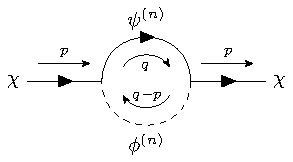
\includegraphics[scale=1.2]{fermionloopscalar.pdf} 
				\label{fig:fermionloopscalar}
			}\qquad \qquad 
			\subfigure[]{
				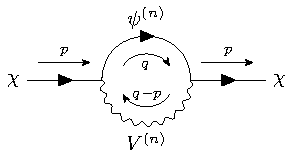
\includegraphics[scale=1.2]{fermionloopvector.pdf}
				\label{fig:fermionloopvector}
			}
			\caption{One-loop diagrams contributing to the wave-function renormalization of light fermion fields in our theories.}
			\label{fig:kineticfermionsbas}
		\end{center}
\end{figure} 
%
Relatedly, in a theory with a supersymmetric spectrum, the on-shell bosonic content equals that of the fermions, such that one would expect the towers to come along with their respective superpartners. Thus, if e.g., $\chi$ in Figure \ref{fig:fermionloopscalar} is a massless gaugino in a 4d $\mathcal{N}=1$ gauge theory, it would couple to both supersymmetric fields belonging to the same charged chiral multiplet. Moreover, this kind of Yukawa couplings associated to supersymmetrized gauge interactions involve the gauge charges precisely like their vector partners do\cite{Wess:1992cp}, namely the Yukawa couplings are of the form $\mathcal{Y}_n \propto \i n$. %Hence, let us turn first to the computation of the relevant loop diagrams.

\subsubsection{Self-energy of a Weyl fermion}
\label{sss:selfenergyfermion}	
Let us compute the wave-function renormalization induced on a chiral fermion $\chi$ by the tower of bosonic and fermionic particles interacting with the former through Yukawa-like couplings of the form discussed in \eqref{eq:fermion&bosonYukawas}. In what follows, we will work with Dirac fermions, such that in order to take into account that the massless spin-$\frac{1}{2}$ field $\chi$ is chiral, it is thus necessary to introduce the  chirality projector $P_{-}=\frac{1}{2}(1-\gamma^{d+1})$, where $\gamma^{d+1}$ is the proper generalization of the four-dimensional $\gamma^5$ to $2k$ dimensions (see Appendix \ref{ap:conventions} for conventions). This way, one can directly work with a Dirac spinor $\mathcal{X}$, whereas the original chiral field can be recovered upon projecting with $P_-$. With this in mind, the interactions in \eqref{eq:fermion&bosonYukawas} can be rewritten in terms of $\{\Psi^{(n)}, \mathcal{X} \}$ as follows
%
\begin{equation}\label{eq:interactionsfermion2}
		\mathcal{Y}_n\ \phi^{(n)} \left( \overline{\Psi^{(n)}} P_{-} \mathcal{X} \right) + \text{h.c.}\, , \qquad  \tilde{\mathcal{Y}}_n\ \left(\overline{\Psi^{(n)}} \gamma^{\mu} P_{-} \mathcal{X} \right) V_{\mu}^{(n)} + \text{h.c.}\, .  
\end{equation}
%
The idea then is to extract the momentum-dependent part of the exact propagator of our massless fermion $\chi$ at one-loop after integrating out such heavy particles (see Appendix \ref{ap:LoopsWeylfermion} for details)
%
\beq\label{eq:Euclexactpropagator}
	S(\slashed{p})= \frac{1}{\i\slashed{p}}\, P_{-} + \frac{1}{\i\slashed{p}}\, P_{-}\, \left(\i\Sigma(\slashed{p})\right)\, \frac{1}{\i\slashed{p}}\, P_{-} + \ldots\ ,
\eeq
%
$\i \Sigma(\slashed{p})$ being the (amputated) Feynman diagram depicted in Figure \ref{fig:kineticfermionsbas}. Notice that this is nothing but the fermionic analogue of $\Pi(p^2)$ shown in eq. \eqref{eq:scalarpropagator}. Therefore, if one wants to isolate the quantum corrections to the kinetic term arising from the loops, one then needs to take a derivative of $\i \Sigma(\slashed{p})$ with respect to the external momentum $p^{\mu}$, and subsequently set $p$ equal to zero.
	
\subsubsection*{The loop computation}
In the following, we will particularize to the case in which the bosonic particle running in the loop is a spin-0 field, as in Figure \ref{fig:fermionloopscalar}, although a similar analysis could be performed for the massive 1-form case. The computation thus involves a tower of Dirac fermions $\{\Psi^{(n)}\}$ of masses $\{m_n^{{\text{f}}}\}$ as well as another one made of complex bosonic scalars $\{\phi^{(n)}\}$ with masses given by $\{m_n^{{\text{b}}}\}$. Hence, the self-energy integral we need to examine for each step $n$ in the infinite tower is the following
%
\beq
	\i \Sigma_n(\slashed{p}) \ = |\mathcal{Y}_n|^2 \int \frac{\text{d}^dq}{(2\pi)^d} \frac{P_{-} \left( -\i \slashed{q} + m_n^{\text{f}}\right) P_{+}}{q^2+(m_n^{\text{f}})^2} \frac {1}{(q-p)^2+(m_n^{{\text{b}}})^2}\ ,
	\label{eq:selfenergychi}
\eeq
%
whilst the relevant contribution to the fermionic propagator reads (see Appendix \ref{ap:LoopsWeylfermion})
%
\beq
	\begin{aligned}\label{eq:Euclwavefunctionfermion}
		\frac{\partial \Sigma_n(\slashed{p})}{\partial p^{\mu}} \bigg\rvert_{p=0} = \frac{-2 |\mathcal{Y}_n|^2 \delta_{\mu \nu} \gamma^{\nu}\ P_{+}}{d} \int \frac{\text{d}^dq}{(2\pi)^d} \frac{q^2}{\left[ q^2 + (m_n^{{\text{f}}})^2 \right] \left[ q^2 + (m_n^{{\text{b}}})^2 \right]^2}\ .
	\end{aligned}
\eeq
%
Notice that by carefully evaluating $\i\Sigma_n(\slashed{p})$ at zero external momentum one can see that \eqref{eq:selfenergychi} vanishes, such that no mass term is generated quantum mechanically at one-loop, as it should be. Additionally, the self-energy includes the projector $P_{+}$, since it is associated to the \emph{chiral} field $\chi$. Let us also stress that the behaviour of the above momentum integral strongly depends on the dimension  of our spacetime. In particular, it can be seen to diverge depending on whether $d\geq4$ or not. In any event, since we are interested in its consequences for the Emergence Proposal, we will impose again some UV cut-off which ultimately will be identified with the species scale, rendering the previous integral finite.
	
Now, in order to study with more detail the kind of corrections induced by the previous diagrams and for future reference, we will first specialize to the easier case in which both towers present identical mass gaps, namely we take $m_n^{{\text{b}}} = m_n^{{\text{f}}} = m_n$. For concreteness, let us show in here the explicit results for the case in which $\Lambda/m_n \gg 1$. The pertinent leading expressions take the form
%
\begin{equation}\label{eq:fermionloopsummary}
		\frac{\partial \Sigma_n(\slashed{p})}{\partial p^{\mu}} \bigg\rvert_{p=0}\,   \sim 
		\left\{\begin{array}{lr}
			-|\mathcal{Y}_n|^2 \gamma_{\mu}\ P_{+}\ \frac{1}{m_n^{4-d}} & \qquad\text{for } d< 4\, ,\\ \\ 
			-|\mathcal{Y}_n|^2 \gamma_{\mu}\ P_{+}\ \log\left( \dfrac{\Lambda^2}{m_n^2}\right) &\qquad \text{for } d= 4\, ,\\ \\ 
			-|\mathcal{Y}_n|^2 \gamma_{\mu}\ P_{+}\ \Lambda^{d-4}&\qquad \text{for } d>4\, .
		\end{array}\right.
\end{equation}
%
These results are analogous to those found for the wave-function renormalization of gauge bosons in eqs. \eqref{eq:1-formloopscalarssummary} and \eqref{eq:1-formloopfermionssummary}. In any case, the more general expression for the one-loop contribution to the fermion self-energy (c.f. eq. \eqref{eq:Euclwavefunctionfermion}) in which the towers have different spins as well as different masses can be found at the end of Appendix \ref{ap:LoopsWeylfermion}.
	
\subsubsection{Generating fermion kinetic terms in 4d }
\label{sss:emergencefermion}
		
As stated above, we cannot give a general expression for the emergent kinetic term of a light fermion field without further specifying the structure of towers and couplings involved in the problem. Therefore, in this section we will restrict ourselves to the case of four spacetime dimensions with the aim of illustrating with a simple toy model how the generation of kinetic terms may arise for massless fermions.\footnote{See \cite{Casas:2024ttx} for recent applications of these ideas in 4d $\mathcal{N}=1$ set-ups arising from string theory.} In order to be as general as possible, we consider here a model which does not impose identical mass gaps for the towers. In particular, we start with two different sets of fermions and bosons exhibiting a structure of the form
%
\beq
	m_n^{\mathrm{b}}\, =\, n\, m_{\mathrm{b}}\, , \qquad m_n^{\mathrm{f}}\, =\, n^{1/p}\, m_{\mathrm{f}}\, , \qquad  \LSP\, \simeq\, N\, m_{\mathrm{b}}\, \simeq\, N^{1/p}\, m_{\mathrm{f}}\, ,
\label{eq:dostorres}
\eeq
%
where we have allowed for $m_{\mathrm{f}}$ to be a priori different from $m_{\mathrm{b}}$. For concreteness, we assume $m_{\mathrm{f}}$ to be greater than $m_{\mathrm{b}}$, but notice that we could alternatively start with the reversed situation in which $m_{\mathrm{f}} \leq m_{\mathrm{b}}$, yielding identical results --- upon exchanging $m_{\mathrm{f}}$ and $m_{\mathrm{b}}$. The case with $p=1$ is indeed quite interesting, since depending on the precise value for $\mathcal{Y}_n$ one can recover the wave-function renormalization of the fermionic components either in 4d $\mathcal{N}=1$ chiral or vector multiplets. 
	
On the other hand, for $p\rightarrow \infty$, one has a tower in which the mass gap between two adjacent levels is much smaller than the scale of the tower itself, namely $\Delta m^{\mathrm{f}}_n \ll m_{\mathrm{f}}$. Notice that with the above parameterization we can actually describe towers with different mass scales, for more generality. We moreover assume the massless fermion $\chi$ to couple to the states comprising both towers through the Yukawa-like couplings displayed in \eqref{eq:fermion&bosonYukawas}, thus leading to the one-loop diagrams shown in Figure \ref{fig:kineticfermionsbas}. However, as already mentioned, the dependence of the Yukawa couplings  $\{\mathcal{Y}_n$, $\tilde{\mathcal{Y}}_n\}$ on the state labelling $n$ is, in general, not fixed by any gauge principle. Hence, in order to accommodate different possibilities we consider here Yukawas of the general form\footnote{There is also the possibility of having $m_{{\text{b}}}=m_{{\text{f}}}$ and $\mathcal{Y}_n = \mu_n = \partial_{\Phi} m_n$, which indeed captures the couplings of a supersymmetric tower to the fermionic component within some massless $\mathcal{N}=1$ chiral multiplet, leading to similar results as in Section \ref{sss:emergencemodulimetric}.}
%
\beq
	\mathcal{Y}_n\, \propto\, n^{1/r}\, .
\eeq
%
For $r=p=1$ one indeed recovers a situation in which both towers share the same mass gap (i.e. $m_{\mathrm{f}}=m_{\mathrm{b}}$ ) and the Yukawa charges grow like $\mathcal{Y}_n \propto n$. %This is precisely the case considered in \cite{Palti:2020tsy}, which mimics the behaviour involving some kind of gauge coupling. 
On the other hand, if $r\rightarrow \infty$, the Yukawa coupling does not depend on the state of the tower and it is just some fixed constant. Now, upon using the third relation in \eqref{eq:dostorres}, one sees that the species scale is related to the masses of the towers as follows
%
\beq
	\LSP^4\, \simeq\, N^{1/p}\, m_{\mathrm{b}}\, m_{\mathrm{f}}\, \Mpf^2\, ,
\eeq
%
where in four dimensions, the species scale is defined as $\LSP^2 \simeq \Mpf^2/N$. Thus, we obtain
%
\beq
	g_{\chi \chi}\, \sim\,  \sum^{N} n^{2/r}\, \sim\, N^{\frac{2}{r}+1}\, \sim\, \left(\frac {(m_{\mathrm{f}}\Mpf^2)^{1/3}}{m_{\mathrm{b}}}\right)^{\gamma_r}\, ,
\label{eq:metricafermiongeneral}
\eeq
%
where
%
\beq
	\gamma_{r,p}\, =\, \frac {3p(2+r)}{r(4p-1)}\, .
\eeq
%
 Note that by considering different values for $\{r,p\}$ we find the $\gamma$-parameter to lie in the range $1\leq \gamma \leq 3$. For the particular case of $r=p=1$ one gets $m_{\mathrm{b}}=m_{\mathrm{f}}=\Mt$  and $\gamma_{1,1}=3$ yielding\cite{Palti:2020tsy}
%
\beq
	g_{\chi\chi}\, \sim\, \left( \frac {\Mpf}{\Mt}\right)^2\, ,
\eeq
%
which is analogous to the structure found for the gauge kinetic functions. (In particular, if we take $\mathcal{Y}_n = -\i \sqrt{2}\ q_n g$ \cite{Wess:1992cp}, as in the gaugino case, one obtains agreement with the 1-form wave-function renormalization discussed in Section \ref{sss:emergenceU(1)}.) For towers/charges with a different structure the more general result, i.e. eq. \eqref{eq:metricafermiongeneral}, applies. Still, the take-home message is that fermions may get large wave-function renormalization if at least one of the towers running in the loop is sufficiently light. 

\begin{comment}
    
\subsubsection*{Emergence of kinetic terms for charged scalars}
We already studied above the case of the emergence of kinetic terms  for a particular class of (massless) scalars, namely the moduli fields. There are however, additional scalars in string theory which are not moduli, like e.g. charged scalars in $\mathcal{N}=1$ chiral multiplets in 4d constructions. For moduli fields, the couplings to the towers are typically determined by the first derivative $\partial_\phi m_n(\phi)$ of the mass of each state in the tower with respect to the modulus $\phi$. However, as in the case of fermions discussed above, for generic scalars the coupling to the infinite towers is in general model-dependent.
	
The relevant loops in this case look like `supersymmetric rotations' of those shown in Figure \ref{fig:kineticfermionsbas}. They are therefore obtained by replacing $\chi \rightarrow {\tilde \chi}$ along with $\phi_n\rightarrow {\tilde \phi}_n$ (or $\Psi_n \rightarrow {\tilde \Psi}_n$) in Figure \ref{fig:kineticfermionsbas}(a) and similarly for Figure \ref{fig:kineticfermionsbas}(b). We refrain from presenting a complete calculation for this (related) case, since the relevant results may be obtained directly from those for fermions presented above.

\end{comment}
	
	
\subsubsection{A Weak-Gravity-like conjecture for  Yukawa couplings}
\label{sss:WGCYukawa}

The stronger versions of the Weak Gravity Conjecture propose that in the presence of a $\mathsf{U(1)}$ gauge field along with charged particles, the limit $g\rightarrow 0$ is singular and should be accompanied by (infinite) towers of states becoming light. A similar question that can arise is what happens with Yukawa couplings, namely when some of these go to zero. In the present discussion we would like to argue that, at least in the context of Emergence, the answer to this question is positive (see \cite{Palti:2020tsy} for similar ideas and \cite{Casas:2024ttx} for recent non-trivial tests in string theory).
	
In the emergence picture one expects every non-vanishing Yukawa coupling already present in the UV (if any) to be generically of order one, up to exponentially suppressed instanton corrections. In fact, this is what is generically found in specific string theory constructions, see e.g., \cite{Ibanez:2012zz}. Thus, couplings involving three fields in four dimensions will have typically the form $\mathcal{Y}^{\text{UV}}_{ijk}\simeq \mathcal{S}_{ijk}$, with all entries in the matrix $\mathcal{S}$ being essentially of $\mathcal{O}(1)$, such that no hierarchies of Yukawa interactions would appear at this level. Therefore, any hierarchical behaviour (like the ones existing in the SM) would appear as an infra-red effect. Indeed, the above considerations about the generation of kinetic terms for fermions may give us a hint regarding how this issue. We will frame the present discussion for concreteness in an 4d $\mathcal{N}=1$ supersymmetric setting, but most of the results should still be amenable to generalization to non-supersymmetric set-ups with minimal changes. Thus, in such a supersymmetric scenario with a \emph{renormalizable} 4d superpotential, $W (\Phi)= \mathcal{S}_{ijk}\Phi^i\Phi^j\Phi^k$, the properly normalized Yukawa couplings would have the form
%
\beq
	\mathcal{Y}_{i j k}\, =\, \mathcal{S}_{ijk}\,  (g_{i \bar i}g_{j \bar j} g_{k \bar k})^{-1/2}\, .
\eeq
%
where $g_{i \bar i}$ are the K\"ahler metrics of the corresponding (massless) chiral multiplets, which we have taken here to be diagonal for simplicity. We now assume that all these metrics for the massless fields are obtained via the emergence mechanism such that, according to the discussion above, we find
%
\beq
	\mathcal{Y}_{i j k}\,  \gtrsim \,  \mathcal{S}_{ijk} \Mpf^{-\gamma}\left[ \left(\frac {m_{l,i}}{m_{h,i}^{1/3}}\right)^{\gamma_i/2}
	\left(\frac {m_{l,j}}{m_{h,j}^{1/3}}\right)^{\gamma_j/2}
	\left(\frac {m_{l,k}}{m_{h,k}^{1/3}}\right)^{\gamma_k/2} \right]\, ,
\eeq
%
where $\gamma =\sum_i\gamma_i/3$ and $\gamma_i=\frac{3p_i(2+r_i)}{r_i (4p_i-1)}$. Here the subindices $\{h,l\}$ stand for the heaviest and lightest masses in each of the loops, respectively. Now, starting with $\mathcal{S}_{ijk}$ being $\mathcal{O}(1)$, if we take some entry of $\mathcal{Y}_{i j k}$ to approach zero it will imply that some (or all) of the towers have to become nearly massless in Planck units. Hence, the above expression is, in some sense, the Yukawa analogue of the magnetic WGC. Notice  also that, depending on how light each of the $\{i,j,k\}$ towers (which need not be different) is, hierarchies in the Yukawa couplings could naturally arise, even though all components in the UV matrix --- i.e. the $\mathcal{S}_{ijk}$ --- were originally of order one. Thus, one could argue that hierarchies in the Yukawa interactions may be a generic effect in \emph{emergent} EFTs, with essentially the same loops inducing the kinetic terms also providing for the hierarchical behaviour of the set $\{ Y_{i j k} \}$ \cite{Castellano:2023qhp}.
	
If the bosonic and fermionic towers present identical mass gaps and $g_{i \bar i}\sim 1/m_i^2$, as in the case in which they are supersymmetric partners of one another, one has $\gamma_i=\gamma=3$ and 
%
\beq
	\mathcal{S}_{ijk}\, m_im_jm_k\, \lesssim\, \mathcal{Y}_{i j k} \, \Mpf^3\, ,
\eeq	
%
which is again reminiscent of a WGC-like expression for the Yukawa couplings. In particular, it was shown in \cite{Heidenreich:2017sim} that in a 4d $\mathsf{U(1)}$ gauge theory coupled to gravity, the cut-off should be bounded as $\LSP \lesssim e^{1/3}\Mpf$, with $e$ denoting the gauge coupling. Hence, for any charged matter particle with mass $m$ below the cut-off one finds
%
\beq
	m^3\, \lesssim\, \LSP^3\, \lesssim\, e\, \Mpf^3\, ,
\eeq
%
which is a `gauge counterpart' of the above Yukawa constraint for the case of a single tower of states with mass parameter given by $m$. %This parallelism is in fact not a coincidence since, e.g., in a supersymmetric theory the gaugino presents Yukawa couplings (with respect to charged chiral multiplets) of strength controlled by $e$ as well. Since the gaugino kinetic term is equal to the gauge kinetic coupling, the same structure for this Yukawa coupling appears, as discussed above.	  
	
We end this section with an important comment concerning the gauge coupling renormalization. One could naively argue that by applying this idea to the interaction terms coupling the vector boson to some (conserved) current as in e.g., $({\bar \psi}\gamma^\mu A_\mu \psi)$, gauge interactions could also become hierarchical due to possible large corrections to the wave-function renormalization of the charged fermions. Of course, this cannot be the case since the Ward-Takahashi identities associated to the gauge field relate precisely the vertex and the wave-function factors, such that once we sit in a frame with canonically normalized fermions, the apparent hierarchies disappear. On the other hand, there are no a priori Ward-Takahashi identities for Yukawa couplings (unless they come from a gaugino interaction) and thus hierarchies can arise in general due to possibly large anomalous dimensions. 

\section{Emergence in string theory}\label{s:EmergenceStringTheory}

In this section we test the Emergence prescription introduced in Section \ref{s:EmergenceQG} within several concrete string theory constructions. In particular, we consider theories with 8 supercharges in 4d (Section \ref{ss:emergence4d}) and 6d (Section \ref{ss:emergence6d}) arising from Type II and F-theory Calabi--Yau three-fold compactifications, respectively; as well as 7d theories preserving 16 supercharges obtained from M-theory on $K3$, see Section \ref{ss:emergence7dN=1}. As we will see, each of these examples exhibits different singularity structures that may be ultimately resolved by different kinds of towers of states becoming asymptotically light (in Planck units). The computations that we perform rely heavily on the machinery and formulae presented in Section \ref{s:selfenergybosons}, so that we refer oftentimes to the material presented in that section for the technical details. 

\subsection{Emergence in 4d $\mathcal{N}=2$ theories}
\label{ss:emergence4d}

The first realistic set-up where the Emergence mechanism was studied arises in the context of 4d $\mathcal{N}= 2$ theories as obtained from Type II Calabi--Yau compactifications, see Section \ref{s:4dN=2} for details. The focus was originally placed on the large volume/large complex structure singularity \cite{Corvilain:2018lgw,Grimm:2018ohb,Gendler:2020dfp}, since the associated infinite distance degeneration corresponds to a simple circle decompactification to M-theory on the same three-fold (see Section \ref{sss:5dMtheory} for a detailed discussion of the associated effective 5d $\mathcal{N}=1$ supergravity theory).

In the following, we revisit this analysis in light of our considerations from Section \ref{s:selfenergybosons} above. We will pay special attention to the infinite set of states that are necessary so as to generate (via Emergence) the full gauge kinetic function close to the large volume point. Later on, in Section \ref{ss:generalizations} we turn to other infinite distance degenerations probing instead different duality frames of the theory. Finally, in Section \ref{ss:hypermultiplet4d} we briefly discuss the hypermultiplet moduli space of 4d $\mathcal{N}=2$ theories within the present context.

\subsubsection{Preliminary remarks} 

In this section we consider Type IIA string theory on a CY three-fold $X_3$, and we sit ourselves close to the large volume point, i.e. $\mathcal{V}_{X_3} \to \infty$. This corresponds to an infinite distance singularity, where a number of towers of states become exponentially light with the traversed geodesic distance \cite{Font:2019cxq}. Indeed, notice that for a given BPS particle with $n_{2,a}\in \mathbb{Z}$ units of D2-brane charge --- where the subindex $a$ indicates the holomorphic 2-cycle wrapped by the brane --- and $n_0\in \mathbb{Z}$ the corresponding D0-brane charge, the moduli dependence of the mass measured in 4d Planck units is encapsulated by the normalized $\mathcal{N}=2$ central charge
%
\beq\label{eq:centralchargeI}
		\frac{m_{n_{2p}}}{\Mpf} = \sqrt{8\pi } e^{K_{\text{ks}}/2} |\mathcal{Z}_{\text{IIA}}| = \sqrt{\frac{\pi}{ \mathcal{V}_{X_3}}}\, |n_0+n_{2,a} z^a|\, .
\eeq
%
Therefore, for D2-branes wrapping 2-cycles whose volume grows no faster than $\mathcal{V}_{X_3}^{1/2}$, the above central charge vanishes asymptotically, in agreement with our previous claim. Furthermore, using the duality map between the moduli coordinates of Type IIA string theory on $X_3$ and M-theory on $X_3 \times \mathbf{S}^1$ (see Section \ref{sss:IIA/Mthy} below for details on this), we can relate the 4d states \eqref{eq:centralchargeI} with their five-dimensional counterparts
%
\begin{equation}\label{eq:massesD0D2Emergence}
	 \begin{aligned}
				\frac{m_{\text{D0}}}{\Mpf}\, &\, \sim g_s^{-1} e^{\varphi_4}\, \sim\, \frac{1}{\mathcal{V}_{X_3}^{1/2}}\, \sim\, \frac{m_{\text{KK},\, 5}}{\Mpf}\, ,\\
				\frac{m_{\text{D2}}}{\Mpf}\, & \sim\, e^{K_{\text{ks}}/2} |t^a|\, \sim\, \frac{\tilde{t}^a}{\mathcal{V}_{X_3}^{1/6}}\, \sim\, \frac{m_{\text{M2}}}{\Mpf}\, ,
	 \end{aligned}
\end{equation}
%
where in the last expression we have considered a single D2-brane wrapping some 2-cycle and we have set the corresponding axion v.e.v. $b^a$ to zero. Notice that in order to identify the mass of the D2-particles with that of the M2-branes wrapping the same cycles in the Calabi--Yau, we have split the K\"ahler coordinates into the overall volume $\mathcal{V}_{X_3}$, and rescaled moduli $\tilde{t}^a=t^a/\mathcal{V}_{X_3}^{1/3}$, which are subject to the very special geometry constraint (c.f. eq. \eqref{eq:veryspecialgeometry})
%
\beq
 \mathcal{K}_{a b c} \tilde{t}^a \tilde{t}^b \tilde{t}^c \stackrel{!}{=} 6\, .
\eeq
%
Now, given that we are dealing with a decompactification limit on a circle, and that the Kaluza-Klein scale is identified with the mass of the D0-branes, one can readily see that the species scale associated to that tower alone already coincides with the 5d Planck scale, i.e.
%
\beq \label{eq:D0towerEmergence}
		\frac{\LSP}{\Mpf}\, \simeq\, \left( \frac{m_{\text{D0}}}{M_{\text{Pl;}\, 4}} \right)^{1/3}\, \sim\, \frac{1}{\mathcal{V}_{X_3}^{1/6}}\, \sim\, \frac{M_{\text{Pl;}\, 5}}{\Mpf}\, ,
\eeq
%
which verifies $\LSP/\Mpf \to 0$, as expected. Nonetheless, following the general procedure described in Section \ref{ss:MultipleTowers} so as to compute the species scale in the presence of multiple towers, once we have calculated the scale associated to the lightest set of states, we should compare it with the characteristic mass of the subsequent lightest tower. In the large volume limit, the next-to-leading one would correspond to the aforementioned set of D2-D0-particles. However, as can be seen from eq. \eqref{eq:massesD0D2Emergence} above, the mass of a wrapped D2-brane is already of the order of the species scale --- if we keep the $\{ \tilde{t}^a\}$ fixed and finite. This means, in turn, that the condition \eqref{eq:algorithmstops} is saturated, such that accounting for this extra set of states as well does not change significantly the previously computed species cut-off, since both towers behave additively. 
		
\subsubsection*{The D-brane field content}
		
Having discussed the objects that must be included in the loop computation when exploring the large volume limit, let us now turn our attention to their corresponding field-theoretic content. The basic claim here is that we need to consider both the tower of BPS bound states of D0-branes, whose particle content corresponds to that of massive Kaluza-Klein replicas within a circle reduction from 5d $\mathcal{N}=1$ supergravity; as well as certain fields with spin strictly smaller than 2, which arise from bound states between a single wrapped D2-brane and $n$ D0 modes. 
		
There are in fact several arguments that support these claims, which stem either from the duality between Type IIA string theory and M-theory (c.f. Section \ref{ss:dualitieswithhighersusy}), or rather from a more concrete super-quantum mechanical analysis. Here we will only review the former, whilst a detailed discussion of the super-quantum mechanics of the D0-branes can be found in Appendix C of \cite{Castellano:2022bvr}. Therefore, recalling that Type IIA string theory on $X_3$ is dual to M-theory compactified on $X_3 \times \mathbf{S}^1$, we deduce that the spectrum of (supersymmetric) states in four dimensions must necessarily include the Kaluza-Klein replica of every light field already present in the 5d theory. On the one hand, this implies that there should exist massive KK modes associated to the 5d massless fields, namely a spin-2 multiplet, ($h^{1,1}-1$) vector multiplets, and ($h^{2,1}+1$) hypermultiplets \cite{Cadavid:1995bk}. From the four-dimensional perspective, these states are nothing but the BPS tower of D0-brane bound states. On the other hand, regarding the spectrum associated to the D0-D2 tower, it is clear from the above picture that it should correspond to KK replica of some massive supermultiplet in 5d arising from an M2-brane wrapping the corresponding 2-cycle. There is, however, an extra difficulty due to the fact that its field-theoretic content strongly depends on the moduli space of the supersymmetric cycle wrapped by the 2-brane --- along with its possible flat connections. In any event, for the simplest case in which such moduli space is trivial (i.e. just a point), one can readily see that each step in the tower is associated to a 4d massive hypermultiplet.
		
		
\subsubsection{Emergence of the gauge kinetic function}
\label{ss:4doneloop}
Once we identify the relevant physics taking place in the asymptotic limit of interest, as well as the corresponding towers which should be responsible for such transition, one can proceed by studying whether or not Emergence can work in practice. One possible route would be to use the general results from Section \ref{sss:emergencemodulimetric} to try to reproduce the moduli space metric shown in \eqref{eq:kahlersectormetric}. Here, we focus instead on the more interesting case corresponding to the emergence of the gauge kinetic function, even though both computations are intimately related due to the underlying $\mathcal{N}=2$ structure of the theory. To do so, we hence calculate the one-loop wave-function renormalization of the gauge fields and show that upon integrating out the tower of BPS states (up to the species cut-off) we recover precisely the functions displayed in \eqref{eq:gaugekineticmatrix}.
		
For concreteness, we restrict ourselves to one-dimensional K\"ahler spaces --- i.e. those with $h^{1,1}=1$, where we denote by $z=b+\i t$ the corresponding K\"ahler modulus, whereas the overal volume reads as $\mathcal{V}_{X_3}=t^3$. In that case, we are left with just two $\mathsf{U(1)}$ gauge fields: the graviphoton, and the one belonging to the unique vector multiplet. Still, let us stress here that in the more general multi-moduli scenario, one can similarly probe the large volume regime by splitting the K\"ahler moduli into the volume scalar and rescaled coordinates, see Section \ref{sss:IIA/Mthy} for details. Thus, we conclude that the physics of the $\mathcal{V}_{X_3}\to \infty$ limit is already captured by our current simplified set-up.
		
Therefore, the relevant gauge kinetic matrix that we aim to reproduce takes the following simple form
%
\begin{equation} \label{eq:matrixonemodulus}
	\text{Im}\, \mathcal{N}\, = \frac{\mathcal{K}}{6} \, \left(
		\begin{array}{cc}
			1+3(b/t)^2 & -3b/t^2  \\
			-3b/t^2 & 3/t^2  \\
		\end{array}
	\right) \, ,
\end{equation}
%
where we have substituted the K\"ahler metric 
%
\beq
		G_{z\bar z}= \frac{1}{4t^2}\, ,
\eeq
%
in eq. \eqref{eq:gaugekineticmatrix}. Let us remark two important features exhibited by \eqref{eq:matrixonemodulus} above. First, due to the off-diagonal terms, it implements the phenomenon of gauge kinetic-mixing\cite{Holdom:1985ag,delAguila:1988jz}. Secondly, in the large volume limit (i.e. $t \to \infty$) every entry blows up, such that both vectors become weakly coupled.\footnote{Strictly speaking, when talking about weakly/strongly coupled gauge fields, one refers to the \emph{physical} fields, that is those for which the kinetic functions adopt the canonical form and are thus diagonal. In our example it can be checked that the corresponding eigenvalues of the physical gauge couplings are also vanishing in the $t \to \infty$ limit.} Notice as well that the polynomial dependence on the divergent K\"ahler modulus is different between those terms involving the axion $b$ and those in which it is absent. In the following, we explain how these facts arise naturally when integrating out the tower of D0-branes and D0-D2 particles discussed before.
		 
To show this, we make use of the  renormalization group flow, which induces kinetic mixing when we allow for heavy multi-charged particles to run in the loop, as displayed in Figure \ref{kineticmixing}. Indeed, the gauge kinetic function $f_{AB}^{\text{UV}}$ at a certain UV scale $\Lambda_{\text{UV}}$, is related to the low-energy gauge couplings (for energies well below the masses of the particles) as follows
		%
		\beq \label{eq:oneloopmixing}
		f_{AB}^{\text{UV}}\, =\, f_{AB} - \sum_i \frac{\beta_i}{8\pi^2 \kappa_4^2}\ q_{A}^{(i)} q_{B}^{(i)}\ \log \left(\frac{\Lambda_{\text{UV}}}{m_i}\right)\, ,
		\eeq
		%
where $m_i$ and $q_{A}^{(i)}$ denote the mass and (dimensionless) charge of the $i$-th particle, whereas $\beta_i$ is the corresponding $\beta$-function coefficient. Notice that the kinetic matrix $f_{AB}$ defined here includes a factor of $\kappa_4^{2}$ in the denominator that was explicitly extracted in the definition of $\text{Im}\, \mathcal{N}_{AB}$ within the supergravity action \eqref{eq:IIAaction4d}. This arises since in our conventions the gauge fields are taken to be dimensionless. Additionally, the value of $\beta_i$ depends on the character and degeneracy of the particles running in the loop. For BPS states corresponding to e.g., the D0-D2 tower --- in the simplest one-modulus scenario --- we find $\beta_i= 1$, since the tower is made of charged $\mathcal{N}=2$ hypermultiplets.
		
		%
		\begin{figure}[tb]
			\begin{center}
				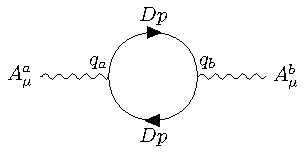
\includegraphics[scale=1.2]{kinetic_mixing.pdf}
				\caption{One-loop diagram with BPS states circulating and giving rise to an effective low-energy kinetic mixing between the different $\mathsf{U(1)}$ vector bosons.}
				\label{kineticmixing}
			\end{center}
		\end{figure}
		%
		
		
Before proceeding with the computation, let us make an important remark about gauge charges, since their precise value depends on the basis of vector bosons that is used. In particular, the basis defined in eq. \eqref{eq:rotatedbasisvectorfields4d} is better adapted for the present analysis, since the associated field strengths are (locally) exact and therefore well-suited for the renormalization of the propagator. Relatedly, the charges of BPS states running in the loop are quantized (they essentially count the number of D$p$-particles comprising each bound-state), and hence moduli-independent. This is to be contrasted with the usual supermultiplet eigenstates basis (i.e. the graviphoton and the orthogonal gauge fields in the vector multiplets), which have neither locally exact field strengths, nor integrally quantized charges.\footnote{The moduli-dependent shifts in the charge vectors can be understood as e.g., induced D0-charges within the 2-brane worldvolume due to a non-trivial $B_2$-flux along the wrapped 2-cycle, c.f. eq. \eqref{eq:CSWZactionTypeIIA}.}
		
\subsubsection*{The case $b=0$}
		
We start here with the simpler case in which the axion v.e.v. is set to zero, i.e. $b=0$. The gauge kinetic functions \eqref{eq:matrixonemodulus} become thus diagonal, so that there is no kinetic mixing anymore, and the dependence with respect to the saxion field is different for each boson. Let us explain how this matrix appears via Emergence, i.e. by integrating out the tower of D2-D0 bound states with one unit D2-charge and $n$ D0-charge.\footnote{In the notation of Section \ref{sss:emergenceU(1)}, the KK-photon coupling to the D0 tower corresponds to $r=p=1$ and that of the D2-D0 to $r=1,\, p \to \infty$. For the other $\mathsf{U(1)}$, the D2-D0 tower corresponds to $r=p \to \infty$.} Consider first the diagonal terms. Hence, from \eqref{eq:oneloopmixing} we get the following kinetic term for $A^0$ 
%
\beq \label{eq:f00}
		f_{00}\, =\, f_{00}^{\text{UV}} + \frac{\beta}{16 \pi^2} \sum_{-n_{\text{max}}}^{n_{\text{max}}}  \left( \pi \Mpf^2 n^2 \right)\ \log \left(\frac{t^3 \,  \LSP^2}{\pi  \, (n^2+t^2) \, \Mpf^2}\right)\, ,
\eeq
%
where we have substituted eq. \eqref{eq:centralchargeI} for the BPS masses, whereas the quantized charges under $A_0$ are given by $q_0^{(n)}\, =\, n  \sqrt{\pi} \Mpf$. Note that $n_{\text{max}}$ is such that the mass of the heaviest state considered in the tower agrees with the cut-off scale, namely $m_{n_{\text{max}}}^2 \sim \LSP^2 \sim 2 \pi \Mpf^2/ t$, thus implying that $n_{\text{max}} \sim t$. Therefore, by approximating the sum with an integral (which is justified in the asymptotic limit) one recovers the following behaviour for the gauge kinetic function
%
\beq 
		f_{00}\, \simeq\, f_{00}^{\text{UV}} +  \beta \,  \Mpf^2 \, \left(\dfrac{3 \pi - 8}{144 \pi } \right)
		t^3 \sim  \,  t^3 \, \Mpf^2 \, ,
\eeq
%
where in the last step we have assumed (following the Emergence prescription) that the UV-contribution is at most as large as the one-loop piece. Hence, we are able to generate the right asymptotic behavior in the first diagonal entry of eq. \eqref{eq:matrixonemodulus}. Similarly, including the contribution from the tower of D0-particles --- which couples only to $A^0$, for which the mass in the denominator should be substituted as $(n^2+t^2) \, \to n^2$, the same asymptotic dependence $\sim t^3$ is generated.
		
Analogously, we can compute the one-loop correction to the kinetic term associated to the second gauge field, $A^1$, induced by the D0-D2 particles (the D0-branes do not couple to $A^1$). In this case, the mass of the states is the same as before, but the charge is now constant $q_1^{(n)}\, =\,  \sqrt{\pi} \Mpf$ for every mode in the tower. The relevant contribution thus takes the form
%
\beq \label{eq:f11} 
		\begin{aligned} f_{11}\, &=\, f_{11}^{\text{UV}} + \frac{\beta}{16 \pi^2} \sum_{-n_{\text{max}}}^{n_{\text{max}}}  \left( \pi \Mpf^2 \right)\ \log \left(\frac{t^3 \,  \LSP^2}{\pi  \, (n^2+t^2) \, \Mpf^2}\right)\, , \\ &\simeq\, f_{11}^{\text{UV}} + \beta \Mpf^2 \left( \frac{4-\pi}{16 \pi }\right) t \sim   t \, \Mpf^2 \, ,
		\end{aligned}
\eeq
%
where in the last step we have assumed the UV piece to be again subleading. Interestingly, the saxion dependence of the second diagonal component of the gauge kinetic matrix   \eqref{eq:matrixonemodulus} presents the same asymptotic behaviour as the one obtained via Emergence.
		
Let us now turn to the off-diagonal contributions. This is arguably the most interesting piece of the discussion, since it gives a couple of nice insights. First, recall the gauge kinetic matrix is diagonal for $b=0$. However, in principle, since the D0-D2 tower is charged with respect to both $\mathsf{U(1)}$ fields, kinetic mixing may be generated via loops. Thus, if the Emergence mechanism works in this case, it should produce a vanishing one-loop correction when the full tower is included. Indeed, the computation yields
%
\beq \label{eq:f01}
		f_{01}\, =\, f_{01}^{\text{UV}} + \frac{\beta \, \Mpf^2}{4\pi} \sum_{-n_{\text{max}}}^{n_{\text{max}}}    n\ \log \left(\frac{t^3 \,  \LSP^2}{\pi  \, (n^2+t^2) \, \Mpf^2}\right) = f_{01}^{\text{UV}}\,  ,
\eeq
%
where the exact cancellation of the loop terms is due to the fact that we sum from $-n_{\text{max}}$ to $n_{\text{max}}$. %Let us remark the importance of summing over all the states in the tower, as the individual contribution coming from each field is not vanishing, but the cancellation nicely arises when the full tower is taken into consideration. 
Therefore, to match with the exact result \eqref{eq:matrixonemodulus}, we need to impose $f_{01}^{\text{UV}}=0$ in eq. \eqref{eq:f01} above. Crucially, this is precisely the expected UV boundary condition, since the decompactified 5d $\mathcal{N}=1$ theory obtained by M-theory on the Calabi--Yau contains no axion-like particles (they arise in 4d as Wilson lines of the 5d vectors along the M-theory circle), and moreover presents no kinetic mixing between the 5d graviphoton and the five-dimensional Einstein-Hilbert term (from which the four-dimensional KK-photon descends).  
		
\subsubsection*{The case $b\neq0$}
		
Let us now turn on the axion v.e.v. and discuss how the preceding results are modified. Notice that once we have non-vanishing axion fields in the vacuum, the gauge kinetic functions include off-diagonal terms, and therefore there is some amount of kinetic mixing between the two vector fields. This, together with the fact that also the $A^0$ gauge coupling is shifted by an axion-dependent amount, are the two main points of the present analysis, and as we will see they can be nicely accounted for in the framework of Emergence. Concerning the light states, the main difference with respect to the $b=0$ case is the $b$-dependent shift in the mass of the D0-D2 tower. More concretely, using \eqref{eq:centralchargeI}, we can see that this is taken into account by the replacement
%
\begin{equation}
\label{eq:shifbneq0}
			m_n^2\, =\, \dfrac{\pi \Mpf^2}{t^3}\left[ n^2 +t^2 \right] \, \longrightarrow \dfrac{\pi \Mpf^2}{t^3}\left[ (n+b)^2 +t^2 \right] ,
\end{equation}
%
which basically means $n \to n+b$ in the denominators inside the logs of eqs. \eqref{eq:f00}-\eqref{eq:f01}. On the contrary, the charges with respect to the fields $\{A^0, A^1\}$ are left unmodified. This seemingly innocuous change is actually at the core of the generation of the axion-dependent terms in the gauge kinetic matrix, as we explain in what follows. %At this point, one could be tempted to say that given the compactness of the axion, and the fact that in the asymptotic limit we are interested in the region where the saxion reaches the infinite-distance boundary of the moduli space (i.e. $t \to \infty$), such modification should not lead to an appreciable change of the results with respect to the $b=0$ situation. However, this intuition turns out to be actually incorrect, given that our one-loop computation was extremely sensitive to the cancellations taking place due to the symmetry upon exchanging $n$ to $-n$. Recall, this was in fact the reason why the off-diagonal terms of the gauge kinetic functions cancelled before. Now, on the other hand, the contribution to the mass that goes as $(n+b)^2$ ceases to be symmetric with respect to the D0 charge, and this is at the core of the generation of the axion-dependent terms in the gauge kinetic matrix.
		
Notice that the structure of the tower is very similar to the one we had before except from a key difference regarding which states lie below $\LSP$. In particular, if we now compute the values of $\{n_{\text{min}}, n_{\text{max}}\}$ so that $m_{n_{\text{min}}}^2 \simeq \LSP^2 \simeq m_{n_{\text{max}}}^2$, we obtain the shifted quantities $n \in [-t-b, t-b]$, such that indeed $n_{\text{min}} \neq -n_{\text{max}}$.\footnote{Notice that CPT does not prevent this asymmetry in the D0-brane charge from happening, given that the would-be hypermultiplets inside the D0-D2 towers are already CPT invariant, such that for a given D0-brane charge $n$, the opposite one appears along with the anti-D2-brane wrapping the same 2-cycle.} Taking this into account, as well as the shift discussed in \eqref{eq:shifbneq0}, we finally obtain
%
\begin{align}\label{eq:4dEmergenceaxion}
			f_{11}&\, \simeq\, f_{11}^{\text{UV}} + \beta \Mpf^2 \left( \frac{4-\pi}{16 \pi }\right) t\, \sim\,   t \, \Mpf^2 \, ,\\ 
			f_{01}&\, \simeq\, f_{01}^{\text{UV}} - \beta \Mpf^2 \left( \frac{4-\pi}{16 \pi }\right) b t\, \sim \, - b  t\, \Mpf^2 \, ,\\
			\begin{split}
				f_{00}&\, \simeq\, f_{00}^{\text{UV}} + \frac{\beta \Mpf^2}{144 \pi } \left[  \left( 3\pi -8  \right) \, t^3 + \left( 4 -\pi \right)\,  b^2 t \right]\, \sim\, (\, C \, t^3 +  \,  b^2 t)\, \Mpf^2\, .
			\end{split}
\end{align}
%
For $f_{11}$ we recover the same result as in the $b=0$ case, as expected. For the mixed term $f_{01}$, however, we get instead a non-vanishing result which is essentially $(-b)$-times the analogous contribution to $f_{11}$, and indeed reproduces \eqref{eq:matrixonemodulus}. (We have set again $f_{01}^{\text{UV}}=0$ in eq. \eqref{eq:4dEmergenceaxion}, since as already discussed there is no such kinetic mixing in the 5d parent theory.) Finally, for the $f_{00}$ component we seem to get the right structure of the gauge kinetic matrix, with a subleading --- but nevertheless diverging --- contribution depending on the axion v.e.v. Notice that we are unable to fix the relative coefficient $C$,  between the two terms in $f_{00}$, since the $t^3$ contribution also receives corrections from the tower of D0-branes alone. %On the one hand, this is to be expected because we should also include the tower of D$0$-branes alone (which couple only to $A^0$), since they can be seen to contribute precisely to the term proportional to $t^3$, but not to the $b^2 t$ term, hence modifying $C$. Moreover, since all our computations (and even the precise definition of the species scale) are defined up to $\mathcal{O}(1)$ factors, one cannot expect to predict accurately the value for $C$. We however expect to get the correct dependence on  the fields, which is precisely what we are able to recover for \emph{every} component of the gauge kinetic matrix \eqref{eq:matrixonemodulus}.
Barring this subtlety, we seem to recover the correct asymptotic structure exhibited by the gauge kinetic matrix \eqref{eq:matrixonemodulus} in this set-up as well.

\subsubsection{Other possible infinite distance limits in 4d}
\label{ss:generalizations}	

In Section \ref{ss:4doneloop} we restricted ourselves to one-dimensional K\"ahler moduli spaces, in which the relevant infinite distance singularity was identified with the large volume point. Moreover, the asymptotically massless tower of states giving rise to the singularity effectively implemented a circle decompactification to 5d M-theory on the same Calabi--Yau three-fold. However, as already commented around eq. \eqref{eq:matrixonemodulus}, the discussion there seems to apply equally well to higher dimensional moduli spaces, as long as we fix the rescaled K\"ahler parameters, $\tilde{t}^a = t^a/\mathcal{V}_{X_3}^{1/3}$, to be finite (and non-vanishing) whilst the volume modulus, $\mathcal{V}_{X_3}$, is taken to infinity.
		
Therefore, one could also ask at this point what happens now if we additionally move close to infinite distance boundaries along the $\tilde{t}^a$ directions as well. Indeed, what one expects is to approach another kind of singular limit, exhibiting a different nearly massless tower dominating the infinite distance regime and thus implementing some other gravitational phase transition. Notice that given that we essentially explore the large volume phase of Type IIA string theory on $X_3$, any other infinite distance singularity that we may encounter there should be present already in the vector multiplet moduli space of M-theory on the same three-fold \cite{Witten:1996qb}. In what follows we will concentrate on two other possible infinite distance boundaries, as studied first in \cite{Lee:2019wij, Corvilain:2018lgw}. These correspond to having a universal fibration structure, where the fibre shrinks (in rescaled coordinates) and is given by an elliptic curve or a K3 surface. These limits were shown to be originally in tension with the Emergence Proposal, and in the following we revisit them, elaborating on several important points which solve all the problems encountered by the authors in \cite{Grimm:2018ohb}.
		
\subsubsection*{The F-theory limit}
\label{sss:IIA-Ftheorylimit}		
Let us start with the $\mathbf{T}^2$-limits of \cite{Lee:2019wij}, in which apart from having $\mathcal{V}_{X_3}\to \infty$, %\footnote{Actually, one can see that such $T^2$-limit belongs to ${\cal M}_{\rm VM}$ without having to take also $\mathcal{V}_{X_3}\to \infty$ (meaning that it is not obstructed by quantum corrections \cite{Lee:2019wij}). However, as noted in \cite{Corvilain:2018lgw, Aspinwall:2002nw, Alim:2012ss, Klemm:2012sx, Huang:2015sta}, such related infinite distance singularity is actually `T-dual' to the large volume one, such that we land again in 5d M-theory on the same (elliptic) CY$_3$, with the towers of D0 and D2-branes of section \ref{ss:preliminary} exchanged.}
the Calabi--Yau exhibits asymptotically certain elliptic fibration
%
\begin{equation}
			\begin{aligned}\label{eq:ellipticcaseEmergence}
				\pi: \qquad \mathbf{T}^2 \hookrightarrow &\;X_{3} \\
				&\;\; \downarrow \qquad , \\ &\;B_{2}
			\end{aligned}
\end{equation}
%
where $\mathbf{T}^2$ denotes the elliptic fibre whose associated rescaled K\"ahler modulus, denoted by $\tilde{t}^0$ here, vanishes asymptotically. Notice that this kind of degenerations correspond to Type III singularities in Mixed Hodge Structure (MHS) language, as discussed in \cite{Grimm:2018ohb, Corvilain:2018lgw} (see also Table \ref{tab:limitsN=2} below).
		
It is easy to see that along the aforementioned class of infinite distance limits, both the D0- and D2-particles present the same asymptotic mass scale (see discussion around eq. \eqref{eq:ellipticmass}), contrary to what happens in the large volume point. Moreover, the D2-branes wrapping the elliptic fibre provide now for an \emph{infinite} number of distinct BPS states, which geometrically is reflected in the fact that the Gopakumar-Vafa invariants associated to the $\mathbf{T}^2$ fibre are (generically) non-zero and constant\cite{Klemm:2012sx, Klemm:1996hh} for each $k\in \mathbb{Z}_{\geq 0}$ (c.f. eq. \eqref{prepotentialIIA})
%
\beq
		n_{\mathbf{k}}^{(0)} = \chi(X_3) = 2 \left ( h^{1,1} (X_3) -  h^{2,1} (X_3) \right)\, ,
\eeq
%.
where $k$ denotes the wrapping number of the D2-brane along the elliptic cycle. Additionally, these two towers can mix, forming bound states with D0 and D2 charges which can in principle run independently as long as the total mass remains below the species scale, $\LSP$. Hence, the present scenario corresponds to the case of multiplicative species (with $p=2$) discussed in Section \ref{ss:MultipleTowers}, such that upon using our formulae \eqref{eq:massmixedsprectra}-\eqref{eq:NtotLQGeff}, one indeed reproduces the behaviour exhibited by the exact gauge kinetic matrix, as we show here. Denoting the divergent modulus by $t$, the mass of the D0-branes --- as well as that of D2-branes wrapping the elliptic fibre --- behave as $m_{\text{D}0}\sim m_{\text{D}2}\sim \Mpf/t$. Using the general formula \eqref{eq:NtotLQGeff} for $d=4$ and $p=2$ we obtain the following behaviour for the species scale and the total number of species
%
\begin{equation}
    \LSP\, \sim\,  \dfrac{\Mpf}{t^{\frac{1}{2}}}\, , \qquad \Ntot\, \simeq \, N_{\mathrm{D}0}\,  N_{\mathrm{D}2} \sim t\, .
\end{equation}
%
Performing now a similar calculation to the one shown in \eqref{eq:f00}, where we compute the contribution of the full tower of D2-D0 particles to the kinetic term of the Kaluza-Klein photon $A^0$, we get
%
\beq \label{eq:f00F-theorylimit}
		f_{00}\, \sim\, \sum_{n_{\text{D}2}}^{N_{\mathrm{D}2}} \sum_{n_{\text{D}0}}^{N_{\mathrm{D}0}}  \left(  \Mpf^2\,  n_{\text{D}0}^2 \right)\, \log \left(\dfrac{t}{n_{\text{D}0}^2 + n_{\text{D}2}^2}\right)\, \sim \,  \Mpf^2 \, t^2\,  ,
\eeq
%
where we used that $N_{\mathrm{D}0} \, \sim \, N_{\mathrm{D}2} \sim t^{1/2}$. Similarly, for the kinetic term of the 1-form $A^1$ that couples to the D2-particles becoming light, we obtain the same parametric behaviour, namely
%
\beq \label{eq:f11F-theorylimit}
		f_{11}\, \sim\, \sum_{n_{\text{D}2}}^{N_{\mathrm{D}2}} \sum_{n_{\text{D}0}}^{N_{\mathrm{D}0}}  \left(  \Mpf^2\,  n_{\text{D}2}^2 \right)\, \log \left(\dfrac{t}{n_{\text{D}0}^2 + n_{\text{D}2}^2}\right)\, \sim \,  \Mpf^2 \, t^2\, ,
\eeq
%
whereas for the mixed terms (in the vanishing axion case) as well as the remaining $\mathsf{U(1)}$ fields --- under which the light D2-D0-particles are not charged --- we obtain vanishing contributions from the quantum corrections. Note that eqs. \eqref{eq:f00F-theorylimit} and \eqref{eq:f11F-theorylimit} indeed reproduce the right field dependence of the gauge kinetic matrix \eqref{eq:gaugekineticmatrix} on the divergent modulus $t$ \cite{Grimm:2018ohb} (see also \cite{Marchesano:2022axe} for a complementary approach).

		
To finish this example, let us just add a few relevant comments about the resolution of the infinite distance singularity. Indeed, as already stressed in \cite{Corvilain:2018lgw}, one expects some partial decompactification to happen upon approaching this Type III limit. The main intuition comes from Type IIA/M-theory duality first, and then from M-/F-theory duality (see Section \ref{ss:dualitieswithlowersusy} for details). Thus, recall that upon taking the $\mathcal{V}_{X_3}\to \infty$ limit and on top of that exploring singularities along the $\tilde{t}^a$ directions, what we are effectively doing is probing the 5d moduli space \cite{Witten:1996qb}. Therefore, since a $\mathbf{T}^2$ limit there leads to a circle decompactification to 6d F-theory \cite{Lee:2019wij}, the natural conclusion here would be to identify this Type III singularity with a nested limit from 4d Type IIA to 6d F-theory. One non-trivial check that can be performed so as to provide evidence for the previous conclusion is to employ the super-quantum mechanical machinery so as to deduce the field-theoretic content associated to the D2-branes wrapping the elliptic fibre (see e.g., Appendix C in \cite{Castellano:2022bvr}). Upon doing so, what one finds is that the moduli space of the elliptic fibre $\mathbf{T}^2$ together with its flat connections is again an elliptically-fibered K\"ahler three-fold, such that the D2-particles contain --- for each $n_{\text{D}2}\in  \mathbb{Z} \setminus \lbrace 0 \rbrace$ --- precisely one massive spin-2 multiplet, $h^{1,1} (B_2)=h^{1,1} (X_3)-1$ massive vector multiplets and $h^{2,1} (X_3)+1$ massive hypermultiplets.
		
\subsubsection*{The emergent Heterotic string limit}
\label{sss:IIA-heteroticlimit}		
Finally, we discuss the so-called $K3$-limits introduced in ref. \cite{Lee:2019wij}, which only exist at large volume (due to large $\alpha'$-corrections) and are characterized by the fact that the three-fold presents an asymptotic fibration structure of the form
%
\begin{equation}\label{eq:K3fibration}
			\begin{aligned}
				\rho: \qquad K3 \hookrightarrow &\;X_{3} \\
				&\;\; \downarrow \qquad , \\ &\;\mathbb{P}^1
			\end{aligned}
\end{equation}
%
where again it is the fibre the one shrinking the fastest in rescaled coordinates, upon taking the singular limit. In MHS language, this set-up corresponds to the Type II singularities discussed in \cite{Corvilain:2018lgw}.
		
The crucial difference here with respect to the previous case is that the leading tower of states now comes from a \emph{critical} emergent Heterotic string \cite{Lee:2019wij}. This string arises from a NS5-brane wrapping the $K3$ fibre, whose effective world-sheet theory precisely contains the spectrum associated to a would-be Heterotic string compactification on $\widehat{K3} \times \mathbf{T}^2$ (or a free quotient thereof)\cite{Harvey:1995rn}. Therefore, upon assuming this limit to correspond in general to an emergent Heterotic string limit (c.f. eq. \eqref{eq:IIA/HETduality4d}) we can run our computations for critical string limits described in Section \ref{sss:emergenceU(1)} (more precisely around eq. \eqref{eq:oneloopstringtowergauge}) in order to reproduce the behaviour of the gauge kinetic matrix \eqref{eq:gaugekineticmatrix} within the present case. In particular, using the general formula for the emergent gauge coupling \eqref{eq:1-formemergencestringytowersgeneral} with the mass scale for the string oscillator modes in the case at hand, which reads $m_{\rm h}\sim \Mpf/t^{1/2}$, we obtain
%
\beq
	\delta \left(\frac {1}{g^2}\right)\, \sim\, \frac {\Mpf^4}{m_{\rm h}^2} \, \sim \, \Mpf^2\, t \, .
\eeq 
%
As expected, this gives rise to the correct asymptotic dependence --- for vanishing axion v.e.v.s, see e.g., \cite{Grimm:2018ohb}. %In fact, upon using the more refined formulae from Appendix \ref{ap:Loops1-form}, we arrive at the same leading result.

\subsubsection{Emergence in the hypermultiplet sector}
\label{ss:hypermultiplet4d}
		
Let us now turn our attention to the other (independent) sector of the moduli space of 4d $\mathcal{N}=2$ EFTs coming from Type II Calabi--Yau three-fold compactifications. In particular, our aim here will be to highlight some interesting points about the consistency of the Emergence Proposal with a ubiquitous phenomenon pertaining to these theories, namely that of instanton corrections (see also \cite{Hamada:2021yxy} for complementary discussions about this point).
		
Due to $\mathcal{N}=2$ supersymmetry, the moduli space of the 4d theory factorizes at the two-derivative level (c.f. eq. \eqref{productmoduli}) between the vector multiplet sector $\mathcal{M}_{\rm VM}$, that is a projective special K\"ahler manifold, and the hypermultiplet sector ${\cal M}_{\rm HM}$, which is a quaternionic K\"ahler manifold instead. This can be found in Section \ref{sss:4dN=2basics}, so that we refer the reader interested in the details to that section. %in the particular case of type IIA on $X_3$, by the collective coordinates $q^p$ in eq. \eqref{eq:IIAaction4d}. In the type IIA set-up one finds precisely $\left( h^{2,1}(X_3)+1\right)$ hypermultiplets, with the universal one including the 4d dilaton, $\varphi_4$, and the extra $h^{2,1}$ ones comprising the complex structure moduli, $z^i$ (see e.g. \cite{Grimm:2005fa} for a precise definition of the 4d fields).
One of the features that makes the hypermultiplet moduli space qualitatively different from its vector counterpart is that it receives a plethora of perturbative and non-perturbative quantum corrections. This is so because it includes in e.g., the Type IIA case, both $\varphi_4$ and the complex structure moduli $\{z^i\}$, which control the action of euclidean D2-branes (i.e. 4d instantons) wrapping minimal 3-cycles in the internal geometry. Therefore, the associated effective 4d action can be heavily quantum-corrected depending on where we sit in moduli space, as summarized in Appendix \ref{ap:hypermetric}. In particular, it was explained in \cite{Marchesano:2019ifh,Baume:2019sry} that a would-be infinite distance point which is present at tree-level in the moduli space geometry can get obstructed or excised from the \emph{exact} $\mathcal{N}=2$ quantum moduli space precisely due to infinitely many instanton corrections that become relevant along the limit.
		
%\subsubsection*{The D4-brane Limit}
%
\begin{figure}[t]
		\begin{center}
			\subfigure[]{
				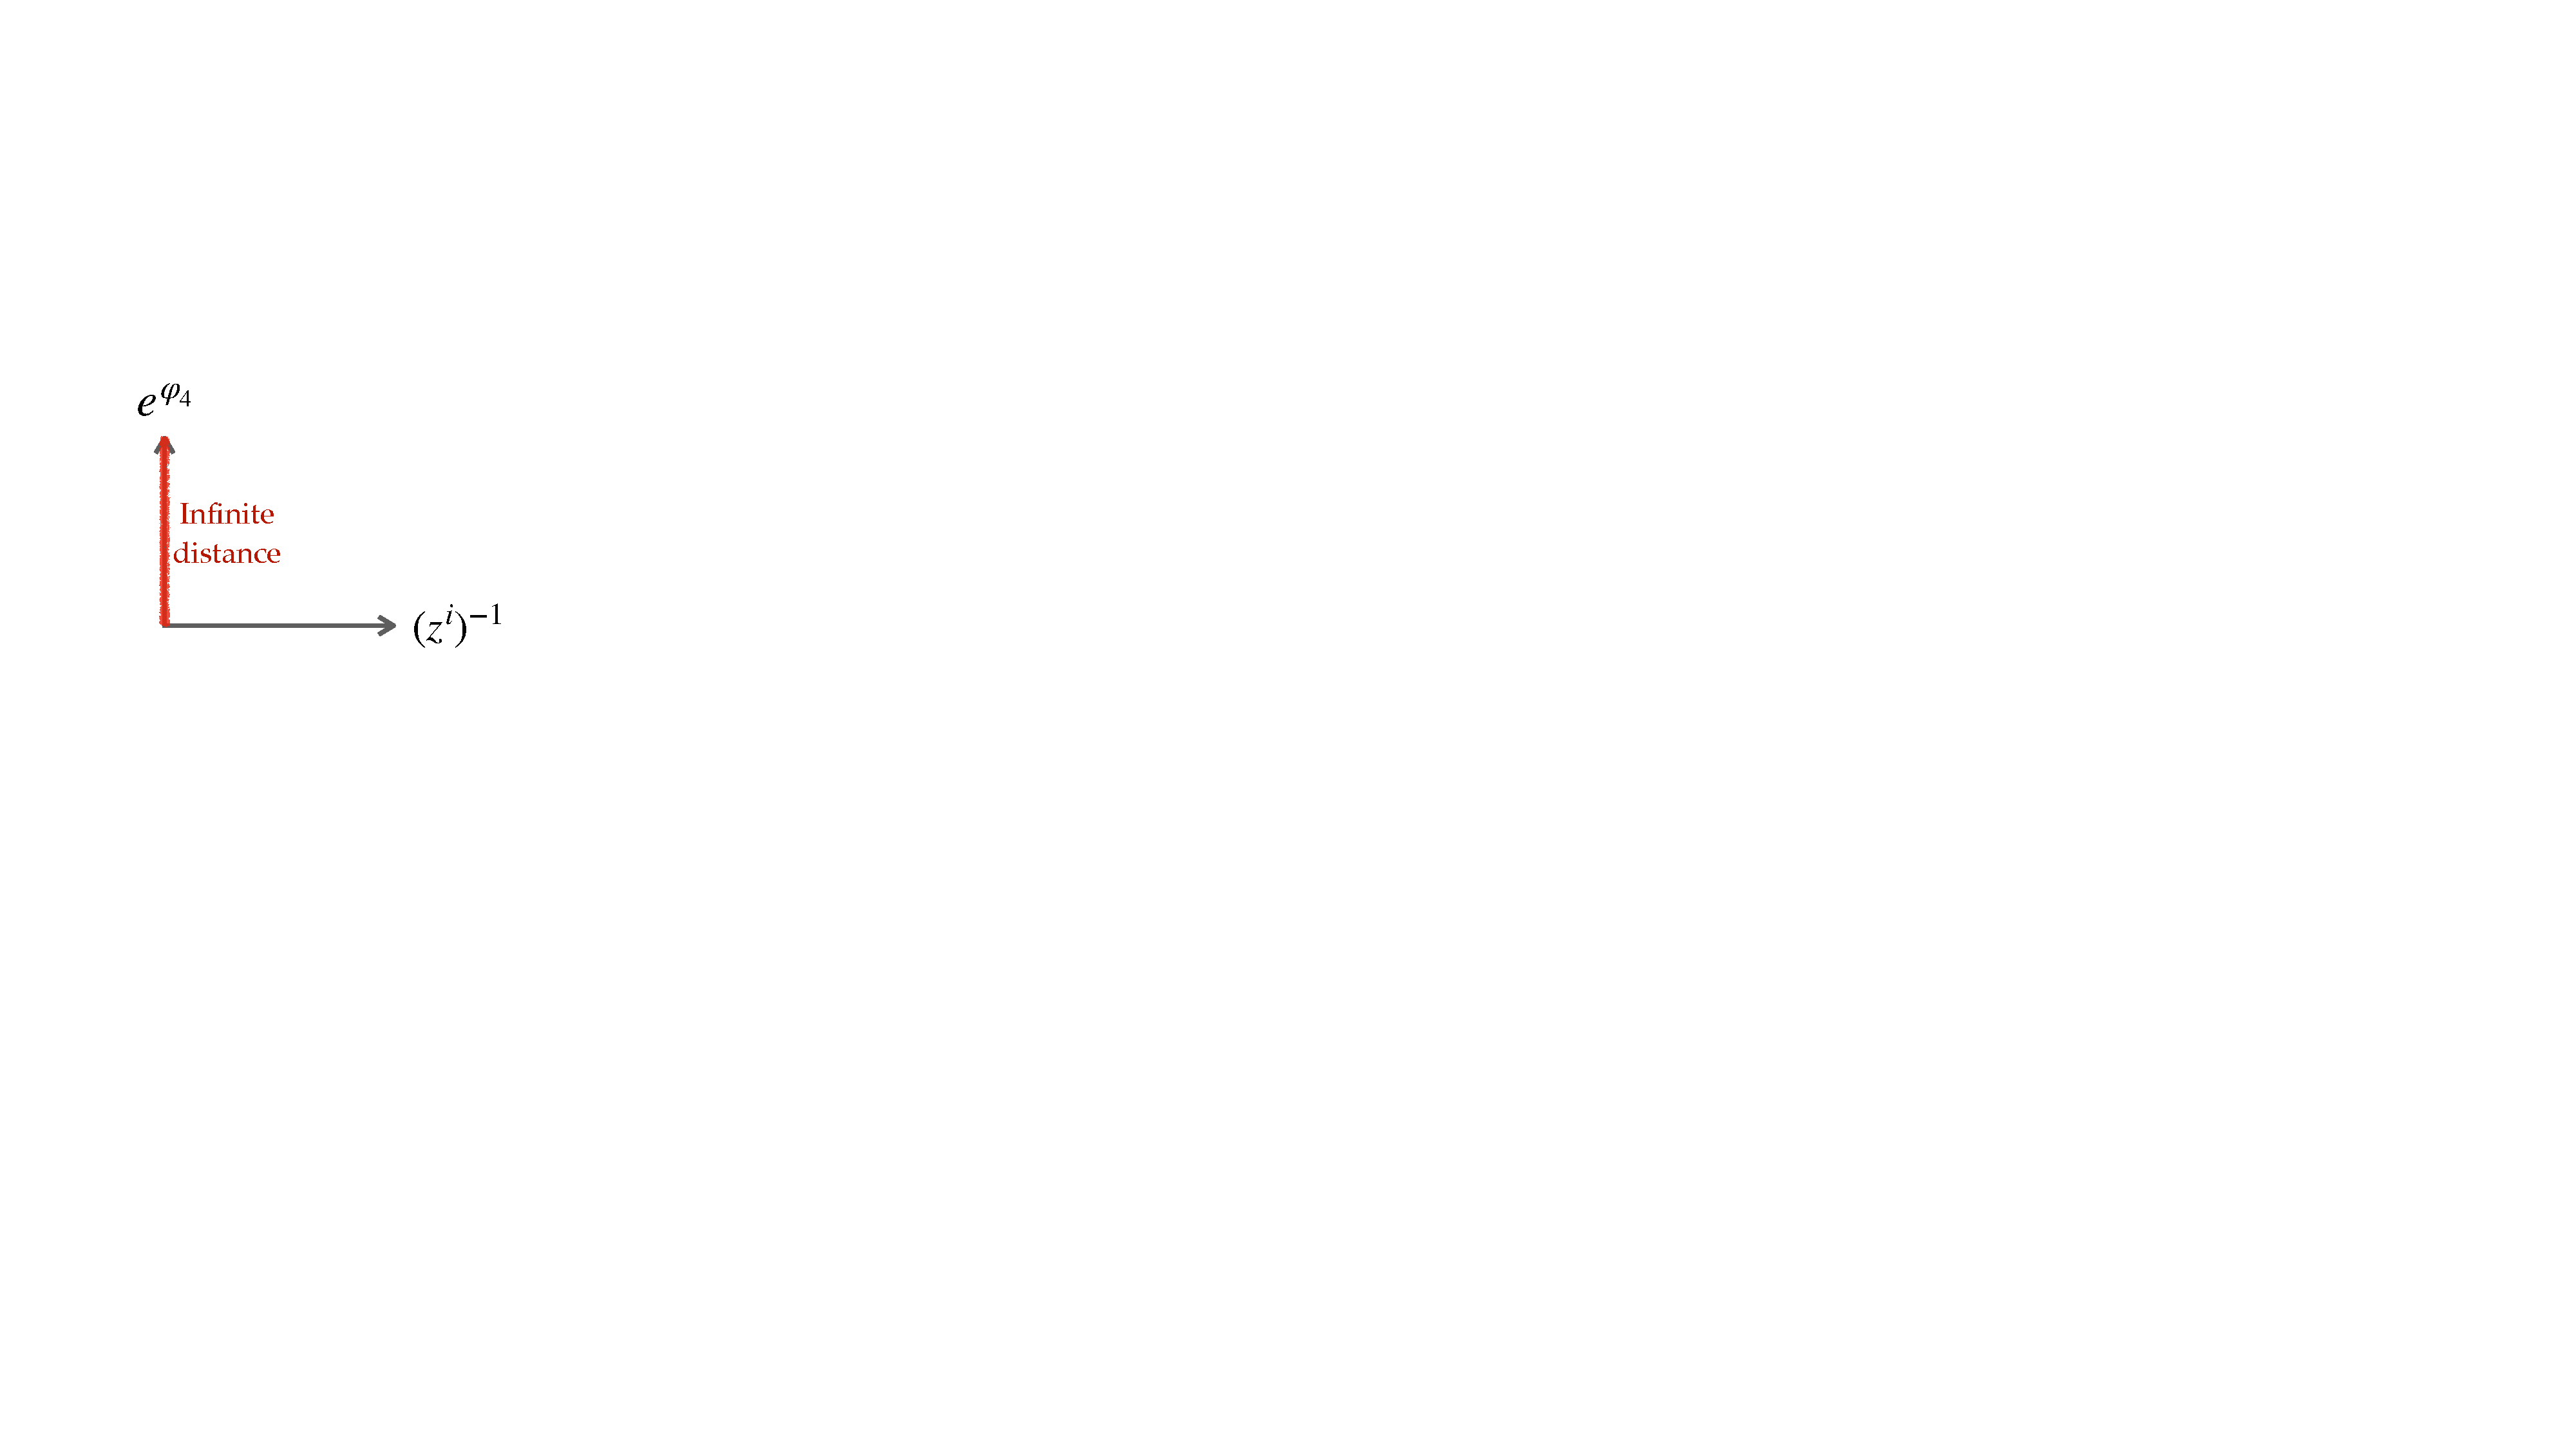
\includegraphics[height=4.5cm]{Instantoncorrections1.pdf} 
				\label{fig:Instantoncorrections1}
			}\qquad \qquad\qquad
			\subfigure[]{
				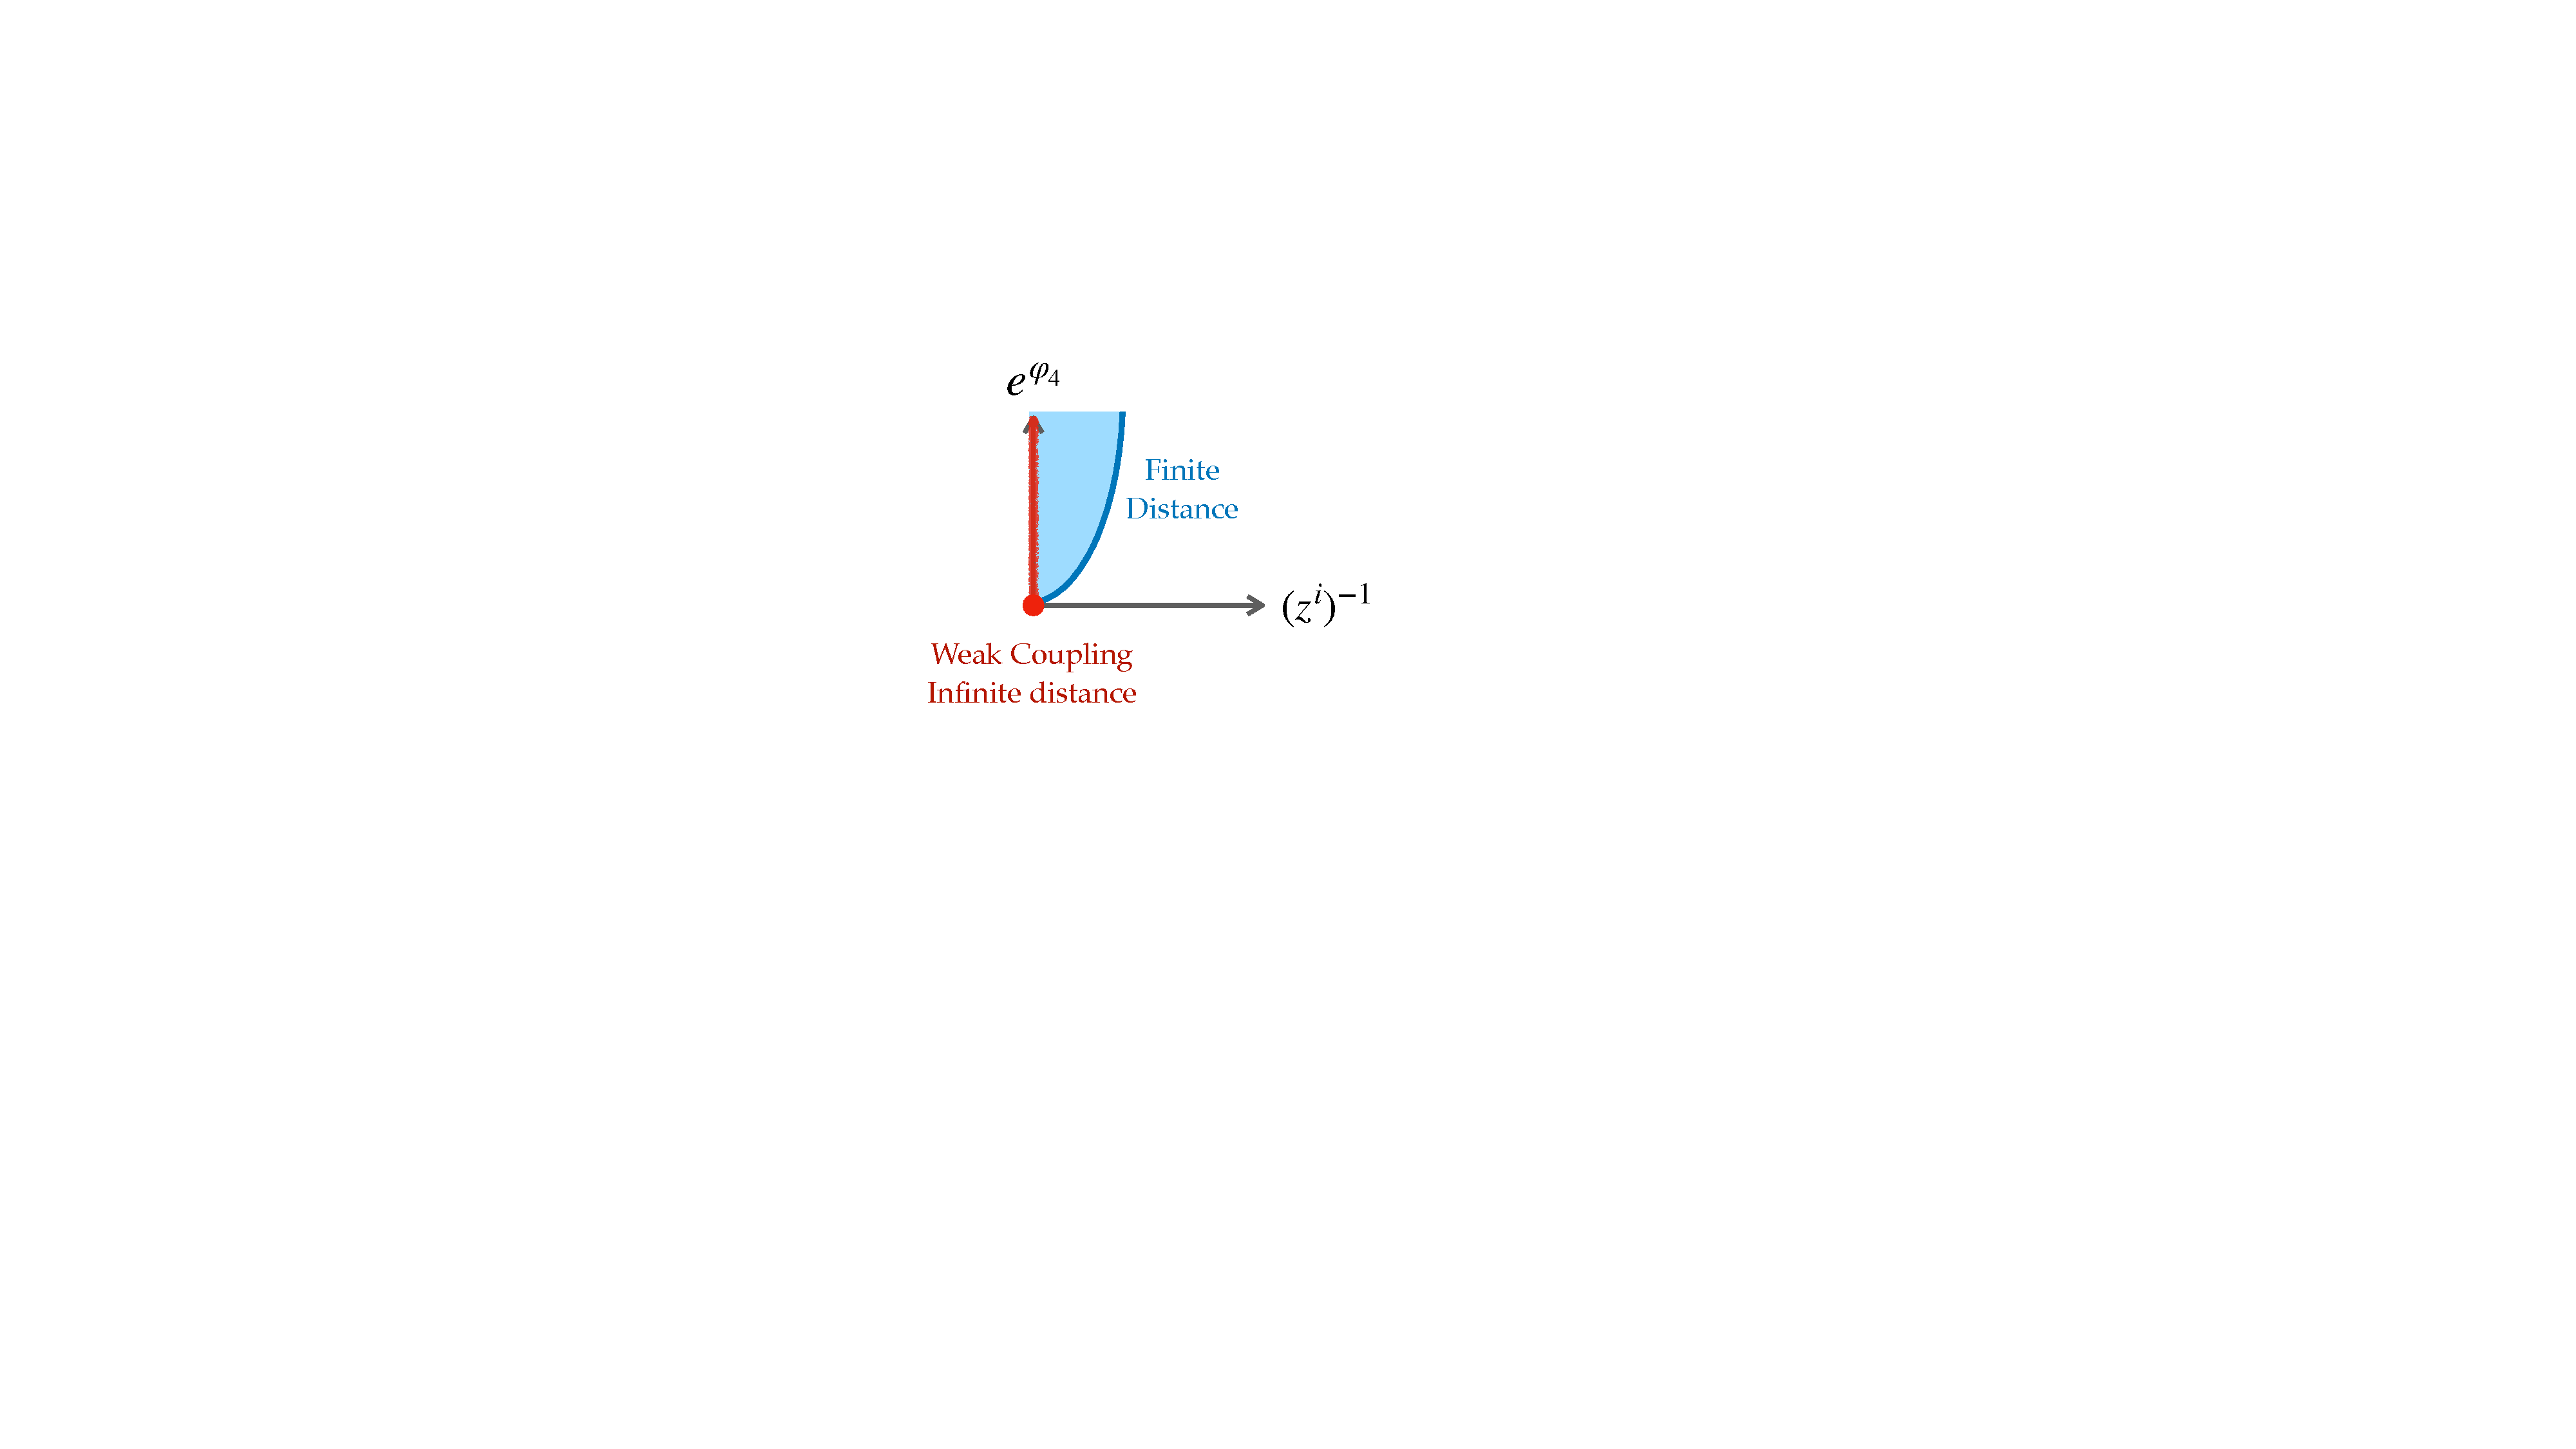
\includegraphics[height=4.5cm]{Instantoncorrections2.pdf}
				\label{fig:Instantoncorrections2}
			}
			\caption{\textbf{(a)} Classical infinite distance limit as $z^i \, \to \,\i \infty$. \textbf{(b)} Including the instanton corrections that become relevant along the limit actually obstructs the would-be classical singularity and leaves only the weak coupling point as an infinite distance boundary.}			
		\label{fig:Instantoncorrections}
		\end{center}
\end{figure} 
%	
Let us briefly review one simple instance in which such obstruction takes place, and try to understand it from the prism of Emergence. We will concentrate on the infinite distance singularity in the mirror symmetric analogue of the D1-limit of \cite{Baume:2019sry}, which was recently investigated in \cite{Alvarez-Garcia:2021pxo}. Hence, consider a geodesic trajectory moving only along the Type IIA hypermultiplet moduli space. The first such trajectory that may come to mind is the one that reaches the large complex structure (LCS) point of the mirror dual Type IIB vector multiplet space, embedded via the c-map within the Type IIA side (we thus keep the 4d dilaton fixed). In the mirror Type IIB compactification, the aforementioned singularity can be understood from Emergence by integrating out D3-branes wrapping some combination of supersymmetric 3-cycles \cite{Grimm:2018ohb, Grimm:2018cpv}. However, in the Type IIA frame, there is no such D3-brane particle states whose mass spectrum is controlled by the complex structure moduli, so that it seems difficult to find an infinite tower which could give rise by quantum corrections to the singular behaviour of the tree-level 4d effective action. 
		
At this point, one could be tempted to conclude that the Emergence Proposal (and even the Distance Conjecture) does not seem to hold in the present case. This is where the analysis of \cite{Baume:2019sry,Alvarez-Garcia:2021pxo} comes to our rescue. It can be seen that, even though we do not have the D3-particles here, there are indeed solitonic strings arising from wrapped D4-branes on non-trivial 3-cycles, together with euclidean D2-instantons, whose tension is controlled precisely by the complex structure moduli.\footnote{As an aside, both strings and instantons happen to be the c-duals of the same D3-particles in the Type IIB side, hence explaining why their tension and action present the same moduli dependence.} The upshot is that along the limit at hand, the action of infinitely many euclidean D2-instantons decreases asymptotically (c.f. eq. \eqref{eq:strongorrections}), such that the tree-level geometry is heavily corrected and, in particular, the infinite distance point at fixed 4d dilaton is excised from the exact quantum moduli space, as schematically displayed in Figure \ref{fig:Instantoncorrections}. Crucially, this is precisely what we would have expected from the Emergence perspective, since we could not find any tower that could generate the tree-level singularity from the beginning. Thus, we can reconcile the absence of a tower with the fact that the infinite distance singularity is actually not present in the exact moduli space.
		
Interestingly enough, even though the LCS singularity at fixed 4d dilaton does not belong to ${\cal M}_{\rm HM}$, one can see that it is actually traded for another (very different) infinite distance degeneration, since the instanton corrections force the dilaton coordinate itself to run towards weak coupling if we insist into approaching the LCS point. The upshot, as explained in \cite{Alvarez-Garcia:2021pxo}, is that an emergent S-dual Type IIA string arising from a D4-brane wrapping the certain shrinking 3-cycle becomes asymptotically tensionless (c.f. eq. \eqref{eq:D4SYZSdual}), and in particular it does so faster than any other critical string in the theory, including the original fundamental one we started with. Therefore, at the end of the day one reaches a new kind of emergent string limit \cite{Lee:2019wij}, which can be reproduced by integrating out the oscillator modes associated to the D4-string --- along with its KK-replicas, in agreement with our expectations coming from Emergence. 
		
		
\subsubsection*{Instanton corrections $\longleftrightarrow$ Emergence loop corrections}
		
In the previous discussion we have used the Emergence Proposal to predict, in some sense, the absence of an infinite distance singularity based on the lack of any infinite tower of particles which could give rise to the latter after being integrated out. To do so, we built upon several results from previous works so as to interpret the would-be infinite distance singularity to be precluded by the presence of an infinite tower of instanton corrections. Our aim in the following is to turn this logic around and use such corrections (which are quantum in nature) to provide more evidence for the picture advocated in the Emergence Proposal.
		
The strategy is to employ the c-map \cite{Cecotti:1988qn,Ferrara:1989ik} so as to relate the D2-instanton corrections in e.g., the Type IIA hypermultiplet sector to one-loop contributions from the infinite tower of D3-particles, in its type IIB vector multiplet counterpart. For concreteness, we skip the technical details of such construction and focus on summarizing the logic behind it. Concretely, the c-map can be understood as some \emph{dressed} T-duality (see Section \ref{ss:dualitieswithhighersusy}) which relates the vector multiplet moduli space of Type IIA on $X_3$ with the hypermultiplet space of Type IIB on the same three-fold, and the vice versa. (This requires from a further $\mathbf{S}^1$-compactification of both theories, and then performing the usual T-duality transformation along said 1-cycle.)
		
What is interesting about the c-map in this context is that it matches quantum contributions to the partition function of the theory as coming from D-instanton sums in one side of the duality, to one-loop corrections associated to integrating out a tower of D-particles on the other. In particular, one can match the instanton number in one theory with the winding number of the particle worldline along the extra $\mathbf{S}^1$ on the dual theory, being the latter moreover related upon Poisson resummation with the Kaluza-Klein modes along the circle. %\footnote{See e.g., \cite{Green:1997as} for a 10d analogue, where one-loop D0-brane (higher derivative) corrections in Type IIA map under T-duality to D(-1)-instanton sums in Type IIB string theory.}
This would naturally explain why starting from the Type IIA hypermultiplet sector, where we find that quantum corrections associated to a tower of euclidean D2-instantons smooth out the moduli space around a given point in ${\cal M}_{\rm HM}^{\rm IIA}$, one should analogously obtain an infinite number of D3-particles that resolve the singularity in ${\cal M}_{\rm VM}^{\rm IIB}$, as required by the Emergence Proposal.
		
To close this section, let us mention that this is nothing but a generalization to infinite distance of a well-understood phenomenon in the finite distance case. Namely, as shown in \cite{Ooguri:1996me}, by using the c-map one can understand the resolution of the conifold singularity within Type II string theory either by invoking the appearance of massless BH-like states at that point in the vector multiplet moduli space (see \cite{Strominger:1995cz}), or by a smoothing-out procedure due to a \emph{single} D-instanton in the hypermultiplet moduli space of the c-dual theory.

		
\subsection{Emergence in 6d $\mathcal{N}=(1,0)$ theories}
\label{ss:emergence6d}
		
The purpose of this section is to test the general analysis performed in Section \ref{sss:emergenceU(1)} concerning the wave-function renormalization induced by a tower of string oscillator modes on some $\mathsf{U(1)}$ gauge field under which they are charged. To do so, we consider certain finite volume infinite distance limits in F-theory compactifications on an elliptically fibered three-fold \cite{Vafa:1996xn,Morrison:1996na,Morrison:1996pp}, as studied originally in \cite{Lee:2018urn}, where some gauge coupling tends to zero as well. There, it was shown that any such limit is indeed equi-dimensional (c.f. footnote \ref{fnote:equidimensional}), such that the light spectrum of the theory is dominated by a critical Heterotic string arising from a D3-brane wrapping some vanishing holomorphic 2-cycle. Moreover, (part of) the tower of excitation states associated to this fundamental dual string is the one satisfying both the Distance and the sub-Lattice Weak Gravity conjectures (see Section \ref{s:SwamplandProgram} for details), thus providing the relevant modes for Emergence.  

Let us summarize first the main results of \cite{Lee:2018urn}, which will be thus necessary so as to study the Emergence phenomenon in this scenario. On the one hand, recall that the 6d Planck scale is fixed by the internal geometry in F-theory, in particular by the volume\footnote{In this section we measure all dimensionful quantities in Type IIB 10d Planck units.} of the complex K\"ahler surface $B_2$ which serves as the base for the elliptically-fibered CY three-fold, namely
%
\beq
\label{eq:Planckmass6d}
	M_{\text{Pl};\, 6}^4 = 4 \pi \mathcal{V}_{B_2}\, \Mpt^4\, .
\eeq
%
On the other hand, the relevant $\mathsf{U(1)}$ field for us arises from 7-branes wrapping certain complex curves $\mathcal{C}$ within $B_2$ (i.e. the discriminant locus $\Delta$ of the elliptic fibration), whose volume sets the corresponding six-dimensional gauge coupling as follows
%
\beq
\label{eq:gaugecoupling6d}
	\frac{1}{g_{\text{IR}}^2} = 2 \pi \mathcal{V}_{\mathcal{C}}\, \Mpt^4\, .
\eeq
%
Therefore, as shown in \cite{Lee:2018urn, Lee:2018spm}, the weak coupling limit for such $\mathsf{U(1)}$ gauge field and with gravity kept dynamical --- which is attained when we blow up the curve wrapped by the 7-brane while keeping the overall volume of the complex surface $B_2$ fixed and finite, require that $B_2$ contains some other rational curve (of vanishing self-intersection), $\mathcal{C}_0$, which moreover intersects $\mathcal{C}$ and whose volume goes to zero as $\mathcal{V}_{\mathcal{C}} \to \infty$. Consequently, a D3-brane wrapping such rational curve gives rise to a solitonic string in the six non-compact dimensions, whose tension is controlled by 
%
\beq
\label{eq:stringtension6d}
	T_{\rm D3,\, str} = 2 \pi \mathcal{V}_{\mathcal{C}_0}\ \Mpt^2\, \sim\, 2 \pi \frac{\mathcal{V}_{B_2}}{\mathcal{V}_{\mathcal{C}}}\ \Mpt^2 \, ,
\eeq
%
and which can be shown to correspond to a weakly coupled dual Heterotic string (compactified on some $K3$ surface), thus having excitation states charged under the 7-brane gauge theory due to the fact that $\mathcal{C}_0$ and $\mathcal{C}$ non-trivially intersect.
		
Our aim here will be to relate the functional form of the gauge coupling in eq. \eqref{eq:gaugecoupling6d} to the appearance of the tower of asymptotically massless charged string states, in the spirit of the Emergence Proposal. In order to do this, we need two basic ingredients: the 6d species scale for this set-up, together with its relation to the characteristic data of the tensionless Heterotic string; and second, the one-loop renormalization of the inverse gauge coupling as well as the spectrum of oscillator modes which are charged under the $\mathsf{U(1)}$ gauge field.
		
To address the first part of the relevant information, we follow the field-theoretic approach introduced in Section \ref{sss:stringtowersspecies}. In particular, evaluating eqs. \eqref{eq:speciescale}-\eqref{eq:Ns} for $d=6$ leads to an expression of the form
%
\beq
		\left ( \frac{M_{\text{Pl};\, 6}}{m_{\text{h}}}\right )^4 =\, \mathsf{N}_{\text{h}}^2 \sum_{n=1}^{\mathsf{N}_{\text{h}}} \text{exp}(\sqrt{n}) \, \sim 2\ \mathsf{N}_{\text{h}}^{5/2} e^{\sqrt{\mathsf{N}_{\text{h}}}}\, ,
\label{eq:maxstringlevel6d}
\eeq
%
where the quantities with the subscript `h' are associated to the emergent critical Heterotic string. In particular, since it is obtained from the wrapped D3-brane discussed above, we have $m_{\text{h}}^2\, =\, T_{\rm D3,\, str}/2 \pi$. Recall also that for such a string tower $\LSP^2 \, \simeq \, \mathsf{N}_{\text{h}} \, m_{\text{h}}^2$.
		
Additionally, the one-loop gauge coupling renormalization at leading order reads as follows
%
\beq
		\label{eq:runninggaugecoupling6d}
		\frac{1}{g_{\text{IR}}^2} = \frac{1}{g_{\text{UV}}^2} + \beta \Mpt^2 \sum_{k=1}^{k_{\text{max}}} q_k^2\, \LSP^2\, ,
\eeq
%
where $\beta$ is a positive numerical prefactor that depends on the specific type of state considered (e.g., whether it is a fermion or a boson, its tensor structure, etc.), and the sum runs over every oscillator state (labelled by the collective index $k$) charged under the $\mathsf{U(1)}$ with quantized charge $q_k$ that appears below the species scale.\footnote{Notice from eq. \eqref{eq:runninggaugecoupling6d} that we have extracted a factor of $\Mpt$ from the gauge charges associated to the oscillator modes of the wrapped D3-brane, so as to have the $q_k$ dimensionless. One can see that this is indeed the correct normalization from e.g., anomaly inflow in the worldsheet of the resulting EFT string\cite{Callan:1984sa,Heidenreich:2021yda}.}  In order to see how the above computation reproduces the expected divergence in \eqref{eq:gaugecoupling6d} upon sending $\mathcal{V}_{\mathcal{C}} \to \infty$, we need a way to parameterize what gauge charges appear for each oscillator level $n$, which in turn controls the mass of the states by the usual linear relation $m_n^2 = 8\pi T_{\rm D3,\, str} (n-1) \,$, as well as their degeneracy. Hence, we borrow some useful results from  \cite{Lee:2018urn}. First, one can estimate the highest charge  appearing at each excitation level $n$ by $q_{\text{max}}(n)= \sqrt{n}$, as frequently happens for Heterotic compactifications.\footnote{\label{fn:modularity}This is essentially fixed by the modular properties of the Heterotic string partition function on the worldsheet torus, see \cite{Lee:2018urn} and references therein.} Secondly, we notice that in concrete examples, such as e.g., F-theory on an elliptic three-fold with base given by a Hirzebruch surface, $B_2=\mathbb{F}_1$, at a given $n$ each value of the charges with $|q| < q_{\text{max}}(n)$ is indeed populated by string states. Taking this kind of behaviour as representative, we need to parameterize the degeneracy $d_{k,n}$ of charged states with charge $k \in \mathbb{Z}$ within each oscillator level $n$. In principle, one would need to extract the precise dependence by studying physical quantities such as the partition function of the tensionless string. Here, however, we take a (possibly oversimplified) parameterization of the form
%
\beq
\label{eq:dmn}
	d_{k,n} \sim f(k)\, e^{\sqrt{n}} \ ,
\eeq
%
with $f(k)$ being any polynomial function with the only restriction that summing over all charges up to $q_{\text{max}}(n)$ within a given step in the tower reproduces the level density of states, i.e. $d_n \sim e^{\sqrt{n}}$. For instance, a simple example for $f(k)$ would be a monomial of the form $f(k) \sim k^p/n^{(p+1)/2}$, with $p \in \mathbb{R}_+$. With these ingredients at hand, we can then perform the summation implicit in eq. \eqref{eq:runninggaugecoupling6d}
%
\beq
\begin{aligned}
			\frac{1}{g_{\text{IR}}^2} & \sim \,  \Mpt^2 \,  \LSP^2 \sum_{n=1}^{\mathsf{N}_{\text{h}}} \sum_{k=0}^{\sqrt{n}} k^2 d_{k,n}\, \sim\, \Mpt^2 \,  T_{\rm D3,\, str} \,  \mathsf{N}_{\text{h}} \sum_{n=1}^{\mathsf{N}_{\text{h}}} n\ \text{exp} (\sqrt{n})\\
			&\sim\, \Mpt^2 \, T_{\rm D3,\, str} \, \mathsf{N}_{\text{h}}^{5/2} \text{exp} (\sqrt{\mathsf{N}_{\text{h}}})\, .
		\end{aligned}
\eeq
%
Next, upon substituting eqs. \eqref{eq:maxstringlevel6d}-\eqref{eq:stringtension6d}, together with $m_{\text{h}}^2\, =\, T_{\rm D3,\, str}/2\pi$, and using also the definition of the 6d Planck mass given in \eqref{eq:Planckmass6d}, we find that the exact same dependence for the $\mathsf{U(1)}$ gauge coupling as in eq. \eqref{eq:gaugecoupling6d} is recovered. %The main difference with respect to the calculation performed in ref. \cite{Lee:2018urn} is that in principle we sum over all the string modes charged under the $\mathsf{U(1)}$, with charges ranging from zero to the maximum value allowed for each oscillator level $n$, with the \emph{assumption} that the degeneracy for such gauge charges can be parameterized by the simple relation displayed in eq. \eqref{eq:dmn}. Instead, in the analysis of \cite{Lee:2018urn} it is assumed that the leading contribution to the wave-function renormalization of the 6d gauge field comes from the states of highest charged within each oscillator level $n$, whilst the rest do not enter neither in the one-loop correction nor in the computation of the species scale. 
		
\subsection{Emergence in 7d $\mathcal{N}=1$ theories}
\label{ss:emergence7dN=1}
		
As our final example, we consider M-theory compactified on a $K3$ surface. The resulting low energy effective field theory (see Section \ref{sss:MtheoryonK3} for a detailed discussion) preserves minimal supersymmetry in seven dimensions, and its bosonic sector is described by the action \eqref{eq:7dMthyK3}. We moreover restrict ourselves to the attractive $K3$ case, since the analysis is enormously simplified and it already serves to prove our point. In that scenario, one can argue that all integral curve classes in $H_2(K3,\mathbb{Z})$ admit holomorphic representatives (see discussion around eq. \eqref{eq:7dMthyattractive}), and therefore they can all give rise to distinguished BPS states from wrapped M2-branes. 

For concreteness, let us reproduce here the scalar-vector-tensor sector of the 7d action, which reads\footnote{\label{fnote:Weylrescaling7d}In order to arrive at the Einstein-framed action \eqref{eq:7dMthyK3scalarvectortensor} after compactifying M-theory on $K3$ one needs to perform the Weyl rescaling $g_{\mu \nu} \to \mathcal{V}_{K3}^{-2/5} g_{\mu \nu}$.}
%
\begin{equation}\label{eq:7dMthyK3scalarvectortensor}
	\begin{aligned}
		S_\text{M-th}^{\text{7d}}\, \supset\, & \frac{1}{2\kappa^2_7} \int \dd^{7}x\, \sqrt{-g}\,  \left( \mathcal{R} - \frac{9}{20} \left(\frac{\partial \mathcal{V}_{K3}}{\mathcal{V}_{K3}} \right)^2 + \mathsf{G}_{a b}\, \partial \tilde{t}^a \cdot \partial \tilde{t}^b\right) -\frac{1}{4\kappa_{7}^2} \int \mathfrak{g}_{a b}F^a \wedge F^b\, ,
	\end{aligned}
\end{equation}
%
where we recall that $J=t^a \omega_a$ denotes the K\"ahler 2-form and $\tilde{t}^a =t^a/\mathcal{V}_{K3}^{1/2}$ are rescaled K\"ahler coordinates. In the following, we will measure every dimensionful quantity in Planck units, keeping in mind that the 7d Planck scale simply reads $M_{\text{Pl};\, 7}^5= \frac{4 \pi}{\ell^5_{7}}$ (see Appendix \ref{ap:conventions} for conventions).

On the other hand, the gauge kinetic matrix $\mathfrak{g}_{a b}$ depends on the K\"ahler moduli as follows		
%
\begin{align}\label{eq:matrix1forms7dMtheory}
			\mathfrak{g}_{a b}= \frac{1}{\mathcal{V}_{K3}^{3/5}} \mathsf{G}_{a b}= \frac{1}{{\mathcal{V}_{K3}^{8/5}}}t_a t_b- \frac{1}{\mathcal{V}_{K3}^{3/5}}\eta_{a b}\, ,    
\end{align}
%
with $\eta_{a b}$ being the intersection form of the corresponding two-fold.

\subsubsection*{F-theory limit}
		
Let us consider first the corner of the 7d moduli space that corresponds to the F-theory limit, where the theory effectively decompactifies to 8d $\mathcal{N}=1$ supergravity. We closely follow the analysis performed in ref. \cite{Lee:2019xtm}, where such limit was carefully studied.

Therefore, suppose that we move in K\"ahler moduli space while keeping the overall $K3$ volume constant, so as to maintain 7d gravity dynamical. The crucial point is that in order to have such an infinite distance, weak coupling point, one of the entries in $\mathfrak{g}_{a b}$ has to blow-up. Indeed, as demonstrated in \cite{Lee:2019xtm}, this requires that the K\"ahler form must behave asymptotically as follows
%
\begin{align}\label{eq:KahlerFtheorylimit}
			J= t^0 \omega_0 + \sum_i \frac{a^i}{2t^0} \omega_i\, , \qquad t^0 \to \infty\, ,    
\end{align}
%
where $\{\omega_0, \omega_i\}$ are generators of the K\"ahler cone, $\{a^i\}$ are some constant numerical factors and $t^0$ is the K\"ahler modulus that scales to infinity in the limit. Additionally, the finite volume requirement imposes the following restrictions on the generators $\{\omega_0, \omega_i\}$ \cite{Lee:2019xtm}
%
\begin{align}
			\omega_0 \cdot \omega_0 = 0\, , \qquad \sum_i \frac{a_i}{2} \omega_i \cdot \omega_0= \mathcal{V}_{K3} + \mathcal{O} (1/(t^0)^2)\, .    
\end{align}
%
Therefore, upon taking as a basis for $H^{1,1}(K3)$ precisely these 2-forms, $\lbrace \omega_a \rbrace = \lbrace \omega_0, \omega_i \rbrace$, one can see that the vector which becomes weakly coupled when we take $t^0 \to \infty$ is precisely $A^0$, whose kinetic term behaves as follows
%
\begin{align}\label{eq:gaugecoupling7d}
			\mathfrak{g}_{0 0} = \frac{(t^0)^2}{\mathcal{V}_{K3}^{8/5}} - \frac{1}{\mathcal{V}_{K3}^{3/5}}\mathcal{C}_0 \cdot \mathcal{C}_0\, .    
\end{align}
%
where the second term is independent of $t^0$. Moreover, it is easy to see that neither $\mathfrak{g}_{i j}$ nor $\mathfrak{g}_{0 i}$ blow up along the limit \eqref{eq:KahlerFtheorylimit}, and hence become negligible when compared to $\mathfrak{g}_{0 0}$. Similarly, since the kinetic terms for the scalar fields $\{ \tilde{t}^a\}$ behave (up to a constant volume prefactor) precisely as the gauge kinetic functions $\mathfrak{g}_{a b}$ (c.f. eq. \eqref{eq:matrix1forms7dMtheory}), one concludes that it is the massless mode parametrized by $\tilde{t}^0$ the one associated to the infinite distance singularity.

Note that in eq. \eqref{eq:gaugecoupling7d} we have introduced a curve class $\mathcal{C}_0$ which belongs the set $\lbrace \mathcal{C}_0, \mathcal{C}_i \rbrace$ dual to $\lbrace \omega_0, \omega_i \rbrace = \lbrace \mathcal{C}^0, \mathcal{C}^i \rbrace$, namely it satisfies
%
\begin{align}
			\mathcal{C}_0 \cdot \mathcal{C}^0 = 1\, , \qquad \mathcal{C}_0 \cdot \mathcal{C}^i = 0\, , \qquad \mathcal{C}_i \cdot \mathcal{C}^0 = 0\, , \qquad \mathcal{C}_i \cdot \mathcal{C}^j = \delta_i^j\, .    
\end{align}
%
Furthermore, it can be shown that the divisor class defined by $\mathcal{C}^0=\omega_0$ contains necessarily a genus-one holomorphic curve whose volume tends to zero along the limit $t^0 \to \infty$ at a rate $\mathcal{V}_{\mathcal{C}^0} = \mathcal{V}_{K3}/t^0 + \mathcal{O} (1/(t^0)^3)$. This means, in particular, that the $K3$ surface admits an elliptic fibration --- over a $\mathbb{P}^1$-base --- of the form depicted in eq. \eqref{eq:fibration}.
		
Additionally, one obtains a tower of asymptotically light BPS particles arising from wrapped M2-branes on the shrinking curve $\mathcal{C}^0$. In fact, due to its $\mathbf{T}^2$-topology, there are indeed bound states of $n$ M2-particles for each $n \in \mathbb{Z}$, such that we obtain a tower of asymptotically light particles with constant degeneracy at each mass level in the spectrum (see \cite{Katz:1999xq} for a more rigorous analysis of these matters). These constitute precisely the Kaluza-Klein replica that effectively implement the circle decompactification along the F-theory limit. Their mass and charge can be computed from the dimensional reduction of the Nambu-Gotto plus Chern-Simons action associated to the M2-brane, yielding (c.f. eq. \eqref{eq:massM2branes})
%
\begin{align}\label{eq:M2particlemassafterWeylrescaling}
			m_{\text{M2}} = \frac{2 \pi}{\ell_{7}} \mathcal{V}_{\mathcal{C}^0}\, \mathcal{V}_{K3}^{-1/5} \sim \frac{2 \pi}{\ell_{7}} \frac{\mathcal{V}_{K3}^{4/5}}{t^0}\, , \qquad \text{as}\ \ t^0 \to \infty\, .    
\end{align}
%
With this, we can now use our general formulae for the one-loop contribution to both the gauge and scalar metrics in the presence of a tower of charged light particles. Thus, starting from eqs. \eqref{eq:KKloopscalarmetricd>6} and \eqref{eq:gaugeemergenceddimensions} and specializing to the seven-dimensional case at hand, we obtain
%
\beq\label{eq:oneloopgaugecoupling7d}
 \begin{aligned}
     \mathsf{G}_{00} &\sim M_{\text{Pl}; 7}^5 \left(\partial_{\tilde{t}^0} \log m_{\text{M2}} \right)^2 \sim M_{\text{Pl}; 7}^5\, \frac{(t^0)^2}{\mathcal{V}_{K3}}\, ,\\
     \frac{1}{g_{\text{IR}}^2} &= \mathfrak{g}_{0 0} \sim M_{\text{Pl}; 7}^5 \left( \frac{2 \pi}{\ell_{7}\, m_{\text{M2}}} \right)^2 \sim M_{\text{Pl}; 7}^5\, \frac{(t^0)^2}{\mathcal{V}_{K3}^{8/5}}\, .
 \end{aligned}
\eeq
%
Above we have used the fact that the M2-particle charges are given by $q_n\, = \,  \frac{2 \pi n}{\ell_{7}}$, as well as the definition of the species scale \eqref{species}. Thus, the infinite distance/weak coupling singularity in the F-theory limit \eqref{eq:KahlerFtheorylimit} can in principle be reproduced via the Emergence mechanism.

\subsubsection*{Emergent string limit}

For completeness, let us also analyze another interesting infinite distance limit that is exhibited by the present theory. It corresponds to the \emph{small radius} point, where the overall $K3$ volume goes to zero size while keeping the set $\{ \tilde{t}^a\}$ fixed and non-degenerate. Indeed, one can argue that this singularity actually corresponds to an emergent string limit \cite{Lee:2019wij}, where an asymptotically tensionless and weakly coupled Heterotic string emerges at infinite distance (see Section \ref{ss:dualitieswithlowersusy} for more on this duality). Such string can be constructed by wrapping the M5-brane on the whole $K3$ surface \cite{Cherkis:1997bx,Park_2009}, with a tension in 7d Planck units which reads as
%
\begin{equation}
	T_{\text{M5,\, str}} = \frac{2 \pi}{\ell_{7}^2}\mathcal{V}_{K3}^{3/5}\, .
\end{equation}
%
It is moreover $\frac12$-BPS and thus couples to some 2-form gauge field $B_2$ which is dual to the massless 3-form potential in \eqref{eq:7dMthyK3}. In fact, upon dualizing the latter following the usual lagrange multiplier procedure, one arrives at an action of the form
%
\begin{equation}\label{eq:7dMthyK3dual}
\begin{aligned}
	S_\text{M-th}^{\text{7d}}\, =\, & \frac{1}{2\kappa^2_7} \int \dd^{7}x\, \sqrt{-g}\,  \left( \mathcal{R} - \frac{9}{20} \left( \partial \log \mathcal{V}_{K3} \right)^2 - G_{i j} \partial \phi^i \cdot \partial \phi^j\right)\\
       &  -\frac{1}{4\kappa_{7}^2} \int \mathcal{V}_{K3}^{-6/5}\, H_3 \wedge \star H_3 + \mathcal{V}_{K3}^{-3/5} \mathsf{G}_{a b} F^a \wedge F^b\, ,
\end{aligned}
\end{equation}
%
where $H_3$ is the field strength of the 2-form to which the M5-string couples, which is given by
%
\begin{equation}\label{eq:H3fieldstrength}
	H_3= dB_2- \frac{1}{3}\eta_{a b} A^a \wedge F^b\, .
\end{equation}
%
Notice that the Chern-Simons term has disappeared in eq. \eqref{eq:7dMthyK3dual} above. This is indeed a usual phenomenom, where upon dualization Chern-Simons couplings get exchanged with transgression terms in the $p$-form field strengths. In the present case, this transgression term shows up in the Bianchi identity of the $B_2$-field, namely
%
\begin{equation}
	dH_3= - \frac{1}{3}\eta_{a b} F^a \wedge F^b\, .
\end{equation}
%
Therefore, performing an exactly analogous analysis as in Section \ref{ss:emergence6d}, one finds an asymptotic behaviour of the form
%
\beq
 \begin{aligned}
     G_{\mathcal{V}_{K3} \mathcal{V}_{K3}} &\sim M_{\text{Pl}; 7}^5 \left(\frac12 \partial_{\mathcal{V}_{K3}} \log T_{\text{M5,\, str}} \right)^2 \sim M_{\text{Pl}; 7}^5\, \frac{1}{\mathcal{V}_{K3}^2}\, ,\\
     \mathfrak{g}_{a b} &\sim \frac{M_{\text{Pl}; 7}^7}{T_{\rm M5}} \mathsf{G}_{a b} \sim \frac{M_{\text{Pl}; 7}^7}{\mathcal{V}_{K3}^{3/5}} \mathsf{G}_{a b}\, .
 \end{aligned}
\eeq
%
for the one-loop contribution to the scalar kinetic term and inverse gauge coupling, respectively.

\begin{comment}
		
\subsubsection*{Classical vs quantum in gravity}	
The example we just discussed is very suggestive of the presumably `fundamental' character of the Emergence Proposal. Typically, when studying some particular example in which Emergence can be quantitatively tested, one arrives at the following question: to which extent the moduli space singularity can be associated to a purely \emph{quantum} phenomenon? 
		
Let us be more specific about this concern. Imagine we started from a $(d+1)$-dimensional EFT weakly coupled to Einstein gravity, in which the dynamics of the spacetime geometry are encoded in the usual Einstein-Hilbert lagrangian
%
\beq
		\mathcal{L}^{d+1}_{\text{EH}}\, =\,  \dfrac{1}{2\kappa_{d+1}^2}\, \sqrt{-\hat g}\, \hat{\mathcal{R}}\, .
\eeq
%
Now, perform a simple $\mathbf{S}^1$--\,compactification, upon which our original light fields (if any) are replicated such that they arrange themselves in the familiar KK prescription. In particular, upon dimensionally reducing the Einstein-Hilbert term above and performing the Weyl rescaling $g_{\mu \nu} \, \to \, \rho^{-\frac{2}{d-2}}\, g_{\mu \nu}$ in order to go to the $d$-dimensional Einstein frame, one obtains the following lagrangian (see e.g. \cite{vanBeest:2021lhn})
%
\beq
		\mathcal{L}^{d}_{\rm EFT}\, =\, \dfrac{1}{2\kappa_{d}^2}\,  \sqrt{- g} \left[ \mathcal{R} -\rho^{-2 \, \left(\frac{d-1}{d-2}\right)}\ F^2 - \left( \frac{d-1}{d-2} \right)\frac{(\partial \rho)^2}{\rho^2}\right]\, ,
\eeq
%
which encodes the dynamics of gravity, the KK-photon $A_{\mu}$ (with field strength $F_{\mu \nu}$) as well as the radius field $\rho$. If we now focus on the lower dimensional theory, we can explore (at least) two kinds of infinite distance singularities, associated to the large/small radius regime. For concreteness, we choose to explore the large radius point, i.e. $\rho \to \infty$, in which our theory naturally decompactifies, and hence the KK tower encoding the replicas of the $d$-dimensional fields become asymptotically light in Planck units. However, by simple dimensional reduction (meaning without caring a priori about would-be quantum corrections associated to the massive towers) one can clearly see that both the field metric singularity as well as the weak coupling behaviour of the KK photon are already apparent at `tree-level'. In other words, both singular behaviours seem to be already present at the classical level.
		
On the other hand, when trying to compute the would-be quantum corrections induced by the towers becoming light below the species scale according to the emergence prescription, what we find (as discussed in Section \ref{s:EmergenceQG}) is that they produce the \emph{same} kind of singular behaviour (i.e. the same moduli dependence) as the one found already at tree-level. Therefore, one cannot be sure about whether the singularity itself arises at the classical or quantum level. In other words, the IR behavior of the scalar metric (weak gauge couplings) obtained by KK reduction at tree-level is `as if' it had been obtained from an EFT with cut-off given by the species scale, in which the metric (gauge coupling) was not necessarily divergent (vanishing), by integrating out the tower of light KK particles that are also present in that theory. The whole point of the stronger versions of the Emergence Proposal is that such divergent (vanishing) behaviour could arise completely as a quantum-mechanical effect, at least in some duality frame.
		
This is precisely why the apparently simple example that we just studied can shed some light on this issue. Here, the precise singularity in the K\"ahler sector of the M-theory compactification is supposedly associated to infra-red divergent loop contributions from (infinitely many) charged states arising from wrapped M2-branes. Such non-perturbative states, which when sufficiently far away from the singularity are well described by a semi-classical black hole geometry (i.e. with an horizon larger than the Planck length/species scale), indeed become asymptotically massless (in 7d Planck units) when approaching the point in moduli space where the wrapped 2-cycle shrinks to zero size. Moreover, as we saw by e.g., looking at the `one-loop renormalization' of the $\mathsf{U(1)}$ gauge coupling in eq. \eqref{eq:oneloopgaugecoupling7d}, the divergences in the effective lagrangian \eqref{eq:7dMthyK3scalarvectortensor} had precisely the right field dependence to be produced by integrating out the tower of would-be BH's up to the species scale. Therefore, in a sense, this seems like a natural generalization to the infinite-distance case of the celebrated conifold singularity arising in the complex structure sector of Type IIB string theory compactified on a CY$_3$ \cite{Strominger:1995cz}. There it was also the case that an apparently classical singularity arising just from Calabi--Yau data was indeed `resolved' by inherently quantum-mechanical effects associated to BH's becoming massless at the conifold point.
		
However, one should remember that the exact same singularity could be understood as a decompactification from 7d to 8d in F-theory on the elliptic $K3$ surface (times the $\mathbf{S}^1$). In such duality frame, our argumentation from the beginning of the present discussion applies, where the tower responsible from the infinite distance singularity, as seen from the seven-dimensional theory is nothing but the KK replica of the F-theory fields along the circle. From this perspective, one could have been tempted to claim that the singularity was classical,\footnote{Let us stress that in F-/M-theory duality it is known that in order to precisely match both effective actions at the two-derivative level, it is sometimes crucial to take into account quantum corrections associated to the KK modes. This happens e.g. in 6d F-theory compactifications on elliptic CY$_3$, where upon reducing on the circle some 5d Chern-Simons terms (which appear to be classical from the M-theory perspective) are fully generated by the KK tower at the quantum level \cite{Bonetti:2011mw,Bonetti:2012fn,Bonetti:2013ela}.} since it already appeared at tree-level just from dimensional reduction.
		
The idea we want to convey though, is that it may not make sense to actually distinguish between classical and quantum gravity, given that the very concept of what is \emph{classical} and what is \emph{quantum-mechanical} is not duality invariant (see e.g., \cite{Vafa:1995fj}). This allows us to speculate with the idea that string theory, or gravity itself, may need from quantum mechanics for consistency from the beginning, such that it may be intrinsically quantum in nature and even do not have a classical limit in the usual sense \cite{Strominger:1995qi}.

\end{comment}

\section{Emergence of higher-dimensional terms}
\label{s:emergenceinteractions}

Up to now we have only considered the generation of kinetic terms in quantum gravitational field theories. However, as we already know, the non-renormalizability of gravity (c.f. Section \ref{ss:basics}) requires necessarily from the presence of higher-dimensional and higher-derivative operators in the effective action. Therefore, a natural question at this point concerns whether those can also be accounted for in the framework of Emergence.

The message we want to convey in this section is that this may well be also the case, for various reasons (see also \cite{Lee:2021qkx} for a complementary discussion). First, as it is familiar from our quantum field theory experience, loop corrections involving massive states generate non-local contributions to the Wilsonian effective action, which can be usually expanded as a power series of local operators of increasing number in derivatives and dimension. Moreover, as argued in Section \ref{ss:classicalfromquantum}, the contribution due an infinite tower of massive modes can yield seemingly classical terms in the effective action once we cut off the sum at the species scale $\LSP$. Hence, a priori tree-level corrections for higher-dimensional operators in string theory could be accounted for upon integrating out the relevant towers of states (see e.g., \cite{Blumenhagen:2024ydy} for a recent analysis regarding the $\mathcal{R}^4$--\,term in maximally supersymmetric theories with $7 \leq d < 11$). Secondly, even operators within the two-derivative lagrangian not corresponding to kinetic terms can be reproduced via Emergence, in principle. Indeed, a particularly interesting instance is that of scalar potentials, which play a key role in determining the possible vacua of the theory. Crucially, it turns out that the generation of such terms can be reformulated as the question of whether non-propagating $(d-1)$-forms (in $d$ spacetime dimensions) \cite{Herraez:2018vae,Bielleman:2015ina,Carta:2016ynn} can get emergent kinetic terms. In this regard, one can argue that e.g., the saxionic dependence of the flux potential in Type IIA Calabi--Yau compactifications can emerge upon integrating out the relevant D$p$-brane states becoming light along the limit of interest (see Section 6 of \cite{Castellano:2022bvr} for details on this procedure).

Here, we choose to focus on higher-derivative operators instead, since their analysis within the Emergence point of view already serves to illustrate various important points.

\subsubsection*{Example: the $\mathcal{R}^2$--\,operator in 4d $\mathcal{N}=2$ theories}

%The authors in \cite{vandeHeisteeg:2022btw} identify $\mathcal{F}_1$ with the (moduli-dependent) number of species $N$, giving various motivations for this. Note that this is also suggested by the Emergence Proposal \cite{Harlow:2015lma,Grimm:2018ohb,Heidenreich:2017sim,Heidenreich:2018kpg}, since upon taking the species scale as the UV cut-off, the one-loop computation of the $\mathcal{R}^2$--\,term in 4d $\mathcal{N}=2$ theories can be shown to behave asymptotically as $\mathcal{F}_1 \sim \sum_{n=1}^{N} \sim N$. 

Let us consider the BPS operator involving two curvature tensors in the 4d efective action obtained from Type IIA on a CY threefold $X_3$. As discussed in Section \ref{s:4dN=2}, this term reads as follows
%
\beq
\label{eq:R2termEmergence}
	S_{\text{IIA}}^{\text{4d}} \supset \int \dd^4x\, \sqrt{-g}\, \mathcal{F}_1(X^A)\, \mathcal{R}_+^2\ +\ \text{h.c.}\, ,
\eeq
%
where $\mathcal{F}_1$ can be identified with the topological free energy at genus one (see Section \ref{ss:threshold4d} for a list of its main properties). For concreteness, we focus here on partial decompactification limits to 6d, where the three-fold exhibits some elliptic fibration of the form shown in \eqref{eq:ellipticcaseEmergence}. Our aim will be to reproduce via certain one-loop computation the relevant functional dependence displayed by $\mathcal{F}_1$ in eq. \eqref{eq:R2termEmergence} above along this set of limits, including subleading (i.e. non-divergent) contributions as well.

Therefore, we recall that in this scenario one finds two infinite towers of asymptotically light states, namely D0 bound states and D2-branes wrapping the elliptic fibre, whose charges run arbitrarily over the integers. Hence, the one-loop contribution to the operator $\mathcal{R}^2$ due to the aforementioned particles is given by (c.f. eq. \eqref{eq:generatingseries})
%
\begin{align}
\label{eq:F1ell}
	\mathcal{F}^{\rm ell}_{1} (z,\bar z)&= -\frac{1}{12} \sum_{(\omega, n) \in \mathbb{Z}^2} \int_{\varepsilon}^{\infty} \frac{\dd\tau}{\tau}\, e^{-\tau m_{\rm D0}^2\left[ (\omega t)^2+(n+ \omega b)^2\right]}\, ,
\end{align}
%
where $z=b+ \i t$ is the K\"ahler modulus associated to the elliptic fibre. Note that we have included in eq. \eqref{eq:F1ell} the contribution due to the zero modes as well, namely those states with $n=\omega=0$ corresponding to the massless particles in the 4d EFT. %which should give rise to an IR divergence (see discussion around eq. \eqref{eq:F1massless}) that will bite us back later on in the computation. 
Moreover, the exponent in the one-loop integral above can be written in a manifestly quadratic form on the integers $\mathbf{n}=(n, \omega)$ as follows
%
\begin{align}
	m_{\rm D0}^2 \left[(\omega t)^2+(n+ \omega b)^2\right] = G^{ij}n_i n_j\, , 
\end{align}
%
where $G$ is a $2\times 2$ matrix with entries
%
\begin{align}
	 G= \frac{1}{(m_{\rm D0}\, t)^2} \left( \begin{array}{cc}
				|z|^2 & -b  \\
				-b & 1  \\
			\end{array} \right)\, , \qquad G^{-1}= m_{\rm D0}^2
 			\left( \begin{array}{cc}
				1 & b  \\
				b & |z|^2  \\
			\end{array} \right)\, ,
\end{align}
%
whilst $G^{-1}$ denotes its inverse. This allows us to rewrite \eqref{eq:F1ell} as
%
\begin{align}
	\mathcal{F}^{\rm ell}_{1}&= -\frac{1}{12} \sum_{\mathbf{n}\in \mathbb{Z}^2} \int_{\varepsilon}^{\infty} \frac{\dd\tau}{\tau}\, e^{-\tau G^{ij}n_i n_j} = -\frac{\pi}{12} \frac{1}{\sqrt{\det G^{-1}}} \sum_{\mathbf{k}\in \mathbb{Z}^2} \int_{\varepsilon}^{\infty} \frac{\dd\tau}{\tau^2}\, e^{-\frac{\pi^2}{\tau} G_{ij}k^i k^j}\, ,
\end{align}
%
where in the second step we have performed a Poisson resummation on the integer-valued vector $\mathbf{n}$ (c.f. footnote \ref{fnote:Poissonresummation}). Next, upon changing the integration variable to $\hat \tau=\tau^{-1}$, we find
%
\begin{align}
	\mathcal{F}^{\rm ell}_{1}&= -\frac{\pi}{12} \frac{1}{m_{\rm D0}^2\, t} \sum_{\mathbf{k}\in \mathbb{Z}^2} \int_0^{\varepsilon^{-1}} \dd \hat \tau\, e^{-\hat \tau \frac{\pi^2}{(m_{\rm D0}\, t)^2} \left| k^1 -k^2 z\right|^2}\, ,
\end{align}
%
where we used that
%
\begin{align}
	G_{ij}k^i k^j= \frac{1}{(m_{\rm D0}\, t)^2} \left[(k^1-b k^2)^2+(k^2 t)^2\right] = \frac{1}{(m_{\rm D0}\, t)^2} \left| k^1 -k^2 z\right|^2\, .
\end{align}
%
Let us first study the UV-divergent term, which is associated to zero-winding number, i.e. $\mathbf{k}=0$. It provides a contribution to $\mathcal{F}^{\rm ell}_{1}$ of the form
%
\begin{align}\label{eq:numberspeciesEmergenceelliptic}
	\mathcal{F}^{\rm ell}_{1}&\, \supset\, -\frac{\pi}{12} \frac{1}{m_{\rm D0}^2\, t} \varepsilon^{-1} = -\frac{\pi}{12} \frac{\Lambda_{\rm sp}}{m_{\rm D0}} \frac{\Lambda_{\rm sp}}{m_{\rm D0}\, t} \sim N_{\rm D0} N_{\rm D2} \sim N_{\rm sp}\, ,
\end{align}
%
where we have substituted $\varepsilon=\LSP^{-2}$ in the second step, and the final result depends on the total number of light species in the theory, as expected from the usual Emergence computations.\footnote{The authors in \cite{vandeHeisteeg:2022btw} identify $\mathcal{F}_1$ with the number of light species $N$ over the entire moduli space, giving various motivations for this. Note that this is precisely suggested by the Emergence computation here performed, c.f. eq. \eqref{eq:numberspeciesEmergenceelliptic}.} The second piece leads to some UV-convergent contribution to $\mathcal{F}_1$, which reads as
%
\begin{align}
	\mathcal{F}^{\rm ell}_{1}& \supset -\frac{1}{12 \pi} \sideset{}{'}\sum_{\mathbf{k} \in \mathbb{Z}^2} \frac{t}{\left| k^1+k^2 z\right|^{2}}\, ,
\end{align}
%
that is moreover modular invariant. Indeed, it can be seen to correspond to the non-holomorphic Eisenstein series of order one (see Appendix \ref{s:SL2Waveforms} for details), and it moreover presents a logarithmic divergence. In this context, though, such divergence is associated to an infra-red effect arising from the inclusion of the massless modes within the sum \eqref{eq:F1ell}. Hence, upon regularization, and requiring modular invariance to be preserved, one finally obtains
%
\begin{align}
	\mathcal{F}^{\rm ell}_{1} (z,\bar z)& = -\frac{\pi}{12} \frac{\Lambda_{\rm sp}}{m_{\rm D0}} \frac{\Lambda_{\rm sp}}{m_{\rm D0}\, t} + \frac{1}{12} \log \left( t \left| \eta(z)\right|^4\right)\, ,
\end{align}
%
which is close to the exact result, see e.g., \cite{Bershadsky:1993ta, vandeHeisteeg:2023dlw}.

\section{Summary}

In the present chapter we have taken the first steps toward a systematic analysis of the idea of Emergence in quantum gravity, as discussed at the beginning of Section \ref{s:EmergenceQG}. A crucial ingredient within this proposal deals with the maximum regime of validity of any gravitational effective field theory, which is captured by the quantum gravity cut-off $\LQG$. This was identified in Chapter \ref{ch:SpeciesIntro} with the species scale $\LSP$, and serves as the physical energy where loop computations must be cut off in gravity. In order to test this, we studied several string theory constructions in diverse dimensions and with different amounts of supersymmetry, thus providing strong evidence for the overall picture advocated in this thesis. 
 
One-loop self-energy computations play an important role in any practical calculation of Emergence, and we addressed them in Section \ref{s:EmergenceQG}. In particular, we analyzed the general case in $d$-dimensions of moduli fields, gauge bosons and (chiral) fermions. As already mentioned, the crucial ingredient so as to get emergent kinetic terms is to use the species scale as the physical cut-off, as well as to sum over all states belonging to the relevant tower(s) becoming light. Remarkably, even though each individual contribution to the kinetic functions gives a quantum loop effect, the final resummed metric turns out to be independent of $\hbar$, due to this very special choice of ultra-violet cut-off. This suggests that perhaps it may not make sense to actually distinguish between classical and quantum gravity, given that the very concept of what is \emph{classical} and what is \emph{quantum-mechanical} is not duality invariant (see e.g., \cite{Vafa:1995fj,Strominger:1995qi}). Furthermore, with this analysis we obtain a number of interesting results. First, we show explicitly that in simple examples one can reproduce the correct leading-order dependence for the known non-linear sigma model metrics of several string theory constructions, in agreement with predictions by the Distance and Weak Gravity conjectures, both in the presence of either Kaluza-Klein or string towers. (In the latter case an approximate field theory inspired approach was employed to treat the higher-spin modes, which should be properly modified using manifestly off-shell string theory techniques, such as e.g., string field theory.) Secondly, we also find that fermion fields can indeed get large contributions to their wave-function renormalization, a fact that may be important for the application of quantum gravity ideas to phenomenology, since most of the Standard Model particles are actually described by spin-$\frac{1}{2}$ fields \cite{Castellano:2023qhp}.  
 
Therefore, we have tested the Emergence Proposal in various selected examples that display different features both in terms of the number of dimensions where the EFT lives, the amount of supersymmetry preserved and the structure of relevant towers appearing along the infinite distance limits. In particular, we have revisited 4d $\mathcal{N}=2$ theories arising from Type IIA Calabi--Yau three-fold compactifications, performing a detailed analysis of the Emergence mechanism in this set-up. In addition, we have studied higher-dimensional examples, including the case of 6d  F-theory compactifications in which the kinetic term for the gauge bosons arise from a solitonic tensionless Heterotic string, as well as 7d theories from M-theory on (attractive) $K3$ surfaces. All the top-down constructions checked so far seem to be naively consistent with Emergence, at least at the level of properly generating the leading (divergent) field dependence, thus suggesting that generic infinite distance singularities may arise non-trivially in quantum gravity as an intrinsic infra-red phenomenon, as originally proposed in \cite{Palti:2019pca,Harlow:2015lma,Grimm:2018ohb,Corvilain:2018lgw,Heidenreich:2017sim,Heidenreich:2018kpg}.

Furthermore, in Section \ref{s:emergenceinteractions} we briefly considered the possibility of generating terms in the effective lagrangian other than the kinetic ones, including scalar potentials and higher-dimensional/derivative operators. The former were discussed in \cite{Castellano:2022bvr} within the context of Type IIA CY compactifications with fluxes, and we refer the reader interested in the details to that reference. The latter also exhibit interesting features that are currently under investigation, see e.g., \cite{Blumenhagen:2023xmk}. To illustrate this point we revisited the behaviour exhibited by the $\mathcal{R}^2$--\,operator in 4d $\mathcal{N}=2$ theories along partial decompactification limits, finding perfect agreement with exact results already present in the literature. 
 
Many important questions remain open before claiming success, so let us finally comment on some of these. First, it would be very interesting to study in more detail how Emergence applies in general for mixed limits where the resolution of the singularity involves a nested chain of decompactifications and/or emergent string limits. Partial progress along this direction has been accomplished recently in \cite{Blumenhagen:2023yws}, where several relevant observations and issues were raised. More generally, understanding how this idea could be realized in AdS spacetimes --- upon using the AdS/CFT correspondence \cite{Maldacena:1997re}, also seems particularly interesting. Moreover, assuming Emergence to pass every test one may think of, the important question arises of what is the fundamental origin of this property as well as its role in the context of the Swampland program. Indeed, the fact that various conjectures lying at the core of the program could be explained via this simple mechanism would point towards some sort of unifying picture in which Emergence, together with the concept of the species scale, could play a major role within the latter. On the other hand, if the strong formulation of Emergence were to be true, it would be necessary to get some insights about the underlying theory of quantum gravity as well as more serious tests in favour of this rather counter-intuitive phenomenon.\footnote{See \cite{Blumenhagen:2023tev,Blumenhagen:2023xmk, Hattab:2023moj,Hattab:2024thi} for recent progress along this direction.}
